\newpage 
%\thispagestyle{empty}
\chapter{Design}

\section{Anforderungen}
Das Design des Antennensystems wird für einen Anwendungsfall im Freiraum dimensioniert. Die Distanz zwischen dem Sender und dem Empfänger soll 10 Meter betragen. Das Übertragungsmedium ist Luft, kann aber idealisiert als Vakuum angenommen werden. Das System soll isotrop abstrahlen und der Gewinn der Empfangsantenne kann mit einem Faktor  1 angenommen werden. Die Antenne soll symmetrisch gespiesen werden und im 2.4 GHz ISM Band arbeiten. Als Quelle dient ein Bluetooth Low Energie Texas Instruments CC2541 Chip mit 0 dBm als Sendeleistung. Als Designkriterien wird eine $S_{11}$ Dämpfung von -10 dB mit einer Bandbreite von mindestens 100 MHz erwünscht und eine Reserve von 6 dB soll in das Linkbudget eingerechnet werden. Die Abbildung \ref{fig:DesignAusgangslage} zeigt die welsentlichen Punkte der Designanforderungen.

%%%%%%%%%%%%%%%%%%%%%%%%%%%%%%%%%
\begin{figure}[!ht]
\begin{center}
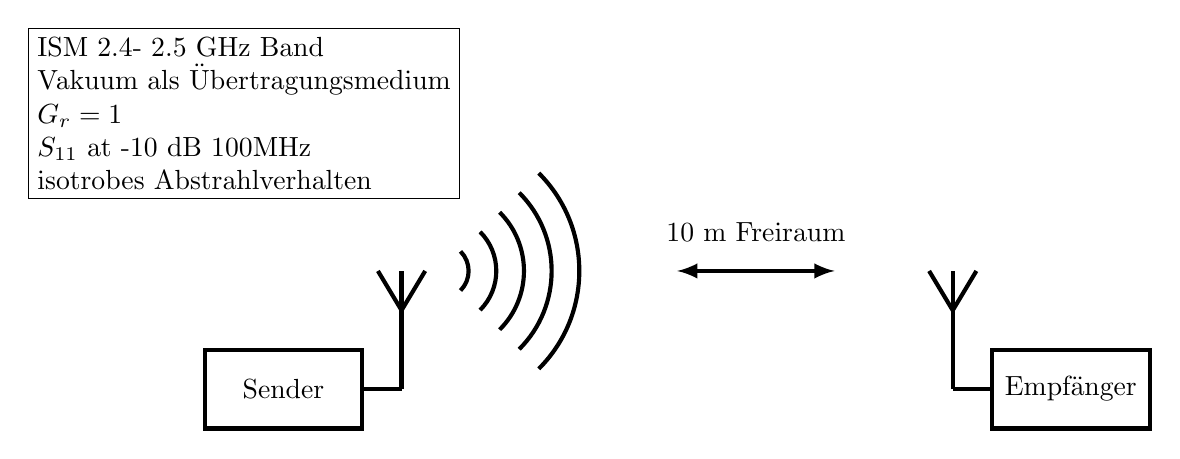
\begin{tikzpicture}
	\draw[line width=1.5pt](0, 0) rectangle (2, 1) node[pos=0.5] {Sender};
	\draw[line width=1.5pt] (2, 0.5) -- (2.5, 0.5);%zuleitung
	\draw[line width=1.5pt] (2.5, 0.5) -- (2.5, 1.5);%Antennenmast
	\draw[line width=1.5pt] (2.5, 1.5) -- (2.2, 2);%Antenne
	\draw[line width=1.5pt] (2.5, 1.5) -- (2.8, 2);
	\draw[line width=1.5pt] (2.5, 1.5) -- (2.5, 2);
	
	\draw[line width=1.5pt, <->, >=latex](6, 2)  -- (8, 2) node at (7, 2.5) {10 m Freiraum};
	
	\draw[line width=1.5pt] (9.5, 0.5) -- (10, 0.5);%zuleitung
	\draw[line width=1.5pt] (9.5, 0.5) -- (9.5, 1.5);%Antennenmast
	\draw[line width=1.5pt] (9.5, 1.5) -- (9.2, 2);%Antenne
	\draw[line width=1.5pt] (9.5, 1.5) -- (9.8, 2);
	\draw[line width=1.5pt] (9.5, 1.5) -- (9.5, 2);
	\draw[line width=1.5pt,decorate,decoration=expanding waves](3, 2) -- (5, 2);
	\draw[line width=1.5pt](10, 0) rectangle (12, 1) node[pos=0.5] {Empfänger};
	\node[draw,align=left] at (0.5,4) {ISM 2.4- 2.5 GHz Band\\ Vakuum als Übertragungsmedium\\ $G_{r} =1$\\ $S_{11}$ at -10 dB 100MHz \\ isotrobes Abstrahlverhalten};
\end{tikzpicture}
\end{center}
\caption{Ausgangslage und Anforderungen an das Design}
\label{fig:DesignAusgangslage}
\end{figure}
%%%%%%%%%%%%%%%%%%%%%%%%%%%%%%%%%%%%%%%%%%

%\subsection{Technische Spezifikationen und Anforderungsliste}
%%\todo{Anforderungskatalogs mit Fest-, Mindest- \& Wunschforderungen}
%\begin{itemize}
%\item Geräte Connect 1
%\item Materialien des Gehäuse ABS Kusnstoff
%\item Volumen des Antennensystems
%\item Wirkungsradius 10m im Freiraum
%\item Richtcharakteristik isotroph
%\item Polarisation linear
%\item Antennen Wirkungsgrad ist zubestimmen
%\item Antennen Gewinn gleich wir der Abstrahl Wirkungsgrad
%\item minimaler Empfangspegel am Transceivers
%\item Transceivers Baustein Texas Instruments CC2541
%\item Sendeleistung
%\item $S_{11} \leq$ 10 dB
%\end{itemize}

\begin{table}[!ht]
\centering
\begin{tabular}{lccr} \toprule 
Nr. & Anforderung & Beschreibung & Wert   \\ 
\midrule
001 & f & ISM Frequenzbereich  & 2.4-2.5 GHz  \\ 
002 & f & Handgerät lxbxh & 142x88x23 [mm]    \\  
003 & f &  Speisung des Antennensystems & symmetrisch  \\  
004 & f & Reflexionskoeffizient der Antenne  at -10B & 100 MHz  \\ 
005 & f & Funkdistanz, Arbeitsradius & 10m   \\ 
006 & f & Linkbudget Reserve & 6dB   \\ 
\bottomrule
  \end{tabular}
  \caption{Anforderungen an das Bluetooth Antennensystem}
  \label{AnforderungenAntenneSystem}
\end{table} 

\section{Design mit bekannten Modellen}

Die in dem Fluginstrument geforderte symmetrische Bluetooth Antenne soll platzsparend im Inneren des Gerätes positioniert sein. Aus diesem Grunde wird eine gedruckte Dipolantenne entworfen. In kleinen elektronischen Geräten sind auf einer Leiterplatte oder auf einem selbstklebenden Kunststoffstreifen gedruckte Antennen von grossem Interesse. Die auf einer Leiterplatte oder einer Folie gedruckten Antennen haben den Vorteil, dass sie sehr kompakt und günstig zu produzieren sind. Zudem sind die Signalwege vom Sende- und Empfangschip zur Antenne sehr kurz. Trotz eines simplen Antennendesign haben Dipolantennen ein annähernd isotropes Abstrahlverhalten. Sie sind als Sende- und Empfangsantennen oft in  tragbaren Geräten eingesetzt. \\

Auf Grund ihrer simplen und kostengünstigen Herstellung sind auf einer Leiterplatte gedruckte Antennen sehr beliebt. Es entstehen nur geringe Kosten, weil die Antenne auf demselben PCB wie die gesamte Gerätelektronik gefertigt wird. Somit wird die Antenne im selben Arbeitsgang wie die Printfertigung hergestellt. Die  Anpassung der Antenne und die strahlenden Antennenelemente sind ebenso Teil der Leiterplatte wie die Elektronikbauteile des Prints. Für ein System, bei dem ein isotropes Abstrahlverhalten gefordert ist, kommen oft Stabantennen zum Einsatz. Um eine gute Abstrahlleistung der Antenne zu erhalten, ist ein $\lambda /2$ Dipol ein viel benützter Ansatz. Dabei erfordert es, dass die effektive mechanische Länge des Dipols etwas weniger als eine halbe Wellenlänge beträgt. Dies kann auf den Verkürzungsfaktor zurückgeführt werden. 
%Ein guter Ansatz ist 0.47 mal die Wellenlänge. 
Zur Berechnung der Länge des in Resonanz betriebenen Dipols kann die  Gleichung \ref{eq:lamba_2_laene_dipol} herangezogen werden.
\todo{Quelle}
\begin{equation}\label{eq:lamba_2_laene_dipol}
L=2l = 0.5 \lambda= 0,5 \dfrac{v}{f}
\end{equation} 
Wobei $v$ die tatsächliche Ausbreitungsgeschwindigkeit der elektromagnetischen Welle im Leiter ist. Diese Geschwindigkeit $v$ hängt von der effektiven dielektrischen Konstante der Umgebung  ab. 
Die effektive  Impulsgeschwindigkeit der Elektronen kann mit der Gleichung \ref{eff_Geschwindigkeit} berechnet werden. 
\begin{equation}\label{eff_Geschwindigkeit}
v = \dfrac{c}{\varepsilon_{eff}}
\end{equation}
Wobei $c$ die Lichtgeschwindigkeit im Vakuum und $\varepsilon_{eff}$  die effektive Dielektrizitätskonstante des umgebenden Mediums ist. Die effektive Dielektrizitätskonstante, einer auf ein Substrat gedruckte Antenne, ist von der  Geometrie und dem Dielektrikum des Substrats abhängig. Die Berechnung der effektiven Dielektrizitätszahl für eine schmale Kupferspur kann aus der Gleichung \ref{eff_epsilon} entnommen werden. 

\begin{equation}\label{eff_epsilon}
\varepsilon_{eff}=\dfrac{\varepsilon_r+1}{2}+\dfrac{\varepsilon_r-1}{2}\left[\left(1+\dfrac{12h}{w}\right)^{-\frac{1}{2}}+0.04\left(1-\dfrac{w}{h}\right)^{2}\right]
\end{equation}
Wobei $h$ die Dicke des Substrats, $w$ die Breite der Antennenstrucktur auf dem Substrat und  $\varepsilon_{r}$ die relative Dielektrizitätskonstante des Substrats ist. 

\section{Designansatz $\lambda$/2 Dipolantenne}  
Unter Verwendung der in Kapitel \ref{sec:Implementierung} erwähnte Gleichung \ref{eq:lamba_2_laene_dipol} soll eine Dipolantenne für die Frequenz 2.45 GHz entworfen werden. Die Antenne wird symmetrisch gespiesen. Die Antenne wird auf eine Leiterplatte gedruckt. Als Substrat des Antennenprints kommt ein  FR-4 PCB mit einem geschätzten  $\varepsilon_r $ von 4.3 bei 1 GHz und einer Substratdicke von 1,5 mm  zum Einsatz. Die Dicke der Kupferschicht beträgt 35 $\mu m$. Die Leiterbahnbreite für den Dipol wird mit 1 mm  definiert.\\

Wird die relative Dielektrizitätskonstante $\varepsilon_{r}$ in die Gleichung \ref{eff_epsilon} eingesetzt, so kann eine effektive Dielektrizitätszahl $\varepsilon_{eff}$  von xxxx berechnet werden.\\

Setzt man die effektive Dielektrizitätszahl $\varepsilon_{eff}$ von xxxxx  in die Gleichung der Elektronengeschwindigkeit aus der Formel \ref{eff_Geschwindigkeit} ein, so erhält man die Geschwindigkeit $v=vvv$. \\
Die Geschwindigkeit $v$  kann in der  Gleichung \ref{eq:lamba_05_langer_dipol} eingesetzt werden. Die Länge des Dipols lässt sich bestimmen als:

\begin{equation}\label{eq:lamba_05_langer_dipol}
L=2l = 0.5 \lambda= 0,5\dfrac{v}{f}=0,5 \dfrac{vvvv}{2.45[GHz]}=bla
\end{equation} 
Für den $\lambda/2$ Designansatz resultiert eine Länge von xx [m].
\subsection{Simulation  verschiedener Geometrien}
Es wurden vier Dipolantennen entworfen. Die Entwürfe sind im EMPIRE XPU erstellt und simuliert worden. Die Antennenabmessungen wurden auf das Simulationsmodel optimiert. Die Länge der Antennen weicht vom $L=2l=\lambda/2$ Ansatz ab. Es wurde versucht, eine optimale Länge für einen Einbau der Antenne für das Fluginstrument  "Connect 1" der Firma Flytec AG zu finden. Die Simulationen gehen von einem 26$\mu$m dicken Kupfer als Antenne aus. Dies enspricht dem 3M Kupferband des Typs "1181 Tape". Die Leimschicht des Klebebands wird vernachlässigt. Als Trägersubstrat dient direkt das ABS Gehäuse \cite{Kupferband}. Für eine Aussage wie das Abstrahlverhalten einer Dipolantenne auf der Längsseite des Fluginstrumentes sich verhaltet, wurde entschieden, dass es nicht nötig ist, die Antennenstrucktur  weder auf ein FR4 Print zu drucken noch ist die aufwändige Fertigung einrer kleinserie von gedruckten Antennen auf einer Klebefolie nötig. Stattdessen wir wie bereits erwähnt das Kupferkelbeband "1181 Tape" verwendet. Es bringt einige Vorteile mit sich: Das Tape ist einfach zu bearbeiten. Es kann mit einer Schere oder mit einem Skalpell die gewünschte Antennform aus dem Tape geschnitten werden. Die geometischen Eigenschaften des Taps sind mit einer Dicke von 26$\mu$m in einem ändlichen Bereich wie eine gedruckte Antenne die auf einer FR4 Kunstharzplatte ist.
\newpage
\subsubsection*{Entwurf}
Die vier Antennen haben alle dieselbe Dicke. Das \glqq 3M 1181 Tape\grqq   hat eine Kupferstärke von 26$\mu$m. Die vier Antennen unterscheiden sich in der Breite der Kupferstreifen und in ihrer Form.\\
Es wurden die folgenden vier Formen simuliert:

\begin{itemize}
\item Dipol 5mm breit und 50.5mm lang
\item Dipol 3mm breit und 50.25mm lang
\item Dipol 1mm breit und 51.25mm lang
\item Dipol 1mm breit und 45.25mm lang mit Dachkapazität
\end{itemize}

%%%%%%%%%%%%%%%%%%%%%%%%%%%%%%%%%
\begin{figure}[!ht]
\begin{center}

\begin{tikzpicture}
\draw[line width=1.5pt,fill=black!30](0, 0) rectangle (2.5, 0.5);
\draw[line width=1.5pt,fill=black!30](2.7, 0) rectangle (5.2, 0.5);
\end{tikzpicture}
\end{center}
\caption{Dipol 5mm breit 50.5mm lang}
\label{fig:Dipol5mmxxlang}
\end{figure}
%%%%%%%%%%%%%%%%%%%%%%%%%%%%%%%%%
%%%%%%%%%%%%%%%%%%%%%%%%%%%%%%%%%
\begin{figure}[!ht]
\begin{center}

\begin{tikzpicture}
\draw[line width=1.5pt,fill=black!30](0, 0) rectangle (2.5, 0.3);
\draw[line width=1.5pt,fill=black!30](2.7, 0) rectangle (5.2, 0.3);
\end{tikzpicture}
\end{center}
\caption{Dipol 3mm breit 50.25mm lang}
\label{fig:Dipol3mm5025lang}
\end{figure}
%%%%%%%%%%%%%%%%%%%%%%%%%%%%%%%%%
%%%%%%%%%%%%%%%%%%%%%%%%%%%%%%%%%
\begin{figure}[!ht]
\begin{center}
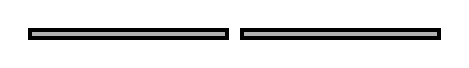
\begin{tikzpicture}
\draw[line width=1.5pt,fill=black!30](0, 0) rectangle (2.5, 0.1);
\draw[line width=1.5pt,fill=black!30](2.7, 0) rectangle (5.2, 0.1);
\end{tikzpicture}
\end{center}
\caption{Dipol 1mm breit 51.25mm lang}
\label{fig:Dipol1mm5125lang}
\end{figure}
%%%%%%%%%%%%%%%%%%%%%%%%%%%%%%%%%
%%%%%%%%%%%%%%%%%%%%%%%%%%%%%%%%%
\begin{figure}[!ht]
\begin{center}
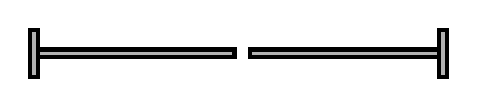
\begin{tikzpicture}
\draw[line width=1.5pt,fill=black!30](1, 0.25) rectangle (3.5, 0.35);
\draw[line width=1.5pt,fill=black!30](3.7, 0.25) rectangle (6.1, 0.35);
\draw[line width=1.5pt,fill=black!30](0.9, 0) rectangle (1, 0.6);
\draw[line width=1.5pt,fill=black!30](6.1, 0) rectangle (6.2, 0.6);
\end{tikzpicture}
\end{center}
\caption{Dipol 1mm breit 45.25mm lang mit Dachkapazität}
\label{fig:Dipol1mm4525langDachkapazität}
\end{figure}
%%%%%%%%%%%%%%%%%%%%%%%%%%%%%%%%%
In der Tabelle \ref{tab:Vergeich_Lambda/2_Freiraum_Geraet} sind einige Antennenparameter und Abstrahlcharakterisiken der verschieden Dipolantennen aufgezeigt. Der $S_{11}$ Wert ist in dB und gibt den maximalen wert der Rückflussdämpfung an. Da die |$S_{11}$| Dämpfung der Antennen im Gerät teilweise nicht über einen Bereich von 100MHz einen  Wert von -10dB erreichen, wird die -10dB Bandbreite hier nicht aufgeführt.
$Z_{ant}$ gibt die simulierte Antennenimpedanz bei einer Frequenz von 2.45GHz an.
Die Abstrahleffizienz $\eta$ gibt in Prozent an die totale Abstrhalleffizenz an. Sie zeigt, wieviel Prozent der zugeführten Leistung der elektromagnetische Welle von der Antennenstruktur abgestrahlt werden kann, wenn die Anregung mit einer idealen 50 Ohm \textit{In Plane} Quelle simuliert wird. Auch $\eta$ wird auf die Abstrahlfrequenz von 2.45GHz bezogen.\\
Die Abstrahleffizienz $\eta$ zeigt bei allen vier Antennen eine Reduktion von ca. 25 $\%$ der Abstrhalleistung wenn die Antenne im Gerät positioniert wird. Weiter macht sich bei allen vier Simulierten Antennen ein Detuninig von mehr als 100 MHz bemerkbar. Dies ist sehr gut in der Abbildung \ref{S11_Vergleich_Simulation_Dipolantenn_freiraum_Geraet} zu entnehmen. 



%%%%%%%%%%%%%%%%%%%%%%%%%%%%%%%
\begin{table}[!ht]
  \centering
  \begin{tabular}{p{8cm} p{2cm} l c c c r} 
  \toprule 
  Antenne                  	& Freiraum im Gerät	 & $S_{11}$[dB]	& $Z_{ant}$[$\Omega$] 	& $\eta$ [$\%$]\\ 
  \midrule
 5mm breit \& 50.5mm lang    	& Freiraum			&	-12.31 @ 2.54		&  	49.7-j27.9		&   	91	\\
            					& im Gerät   			&   -4.92 @ 2.406   		&	17.6+j25.7		& 	62	\\
 3mm breit \& 50.25mm lang    & Freiraum			&    -13.45 @ 2.56  		&	52.9-j28.3		&	91	\\
     						& im Gerät				&  	-5.24 @2.44			&	16+j14.7			&	65	\\
 1mm breit \& 51.25mm lang  	& Freiraum			&    -14.14 @ 2.52    	&	60.4-j23.2		&	93	\\
      						& im Gerät			&  	-5.9 @ 2.45			&	16.5+j6.4		&	68	\\
  1mm breit \& 45.25mm lang
  \& Dachkapazität  		& Freiraum				&   -15.15 @ 2.57      	&	55.4-j29.7		&	90.5	\\
      						& im Gerät			&  	-5.529 @ 2.47		&	15.21j3.8		&	65	\\
 \bottomrule
  \end{tabular}
  \caption{$\lambda/2$ Dipolantennen simuliert im Freiraum und im Gerät}
  \label{tab:Vergeich_Lambda/2_Freiraum_Geraet}
\end{table}
%%%%%%%%%%%%%%%%%%%%%%%%%%%%%%%%%%%
%S11 Parameterder vier Antennen simuliertmit und ohne Gehäuse
%%%%%%%%%%%%%%%
%%%%%%%%%%%%%
%\begin{figure}[!ht]
%	\centering
%	\begingroup
%	\inputencoding{latin1}
%	% This file was created by matlab2tikz.
%
%The latest updates can be retrieved from
%  http://www.mathworks.com/matlabcentral/fileexchange/22022-matlab2tikz-matlab2tikz
%where you can also make suggestions and rate matlab2tikz.
%
\begin{tikzpicture}

\begin{axis}[%
width=4.521in,
height=3.566in,
at={(0.758in,0.481in)},
scale only axis,
separate axis lines,
every outer x axis line/.append style={black},
every x tick label/.append style={font=\color{black}},
xmin=2000000000,
xmax=3000000000,
xlabel={Frequenz in [Hz]},
xmajorgrids,
every outer y axis line/.append style={black},
every y tick label/.append style={font=\color{black}},
ymin=-14,
ymax=0,
ylabel={Amplitude in [dB]},
ymajorgrids,
axis background/.style={fill=white},
title={$\text{Simulation des  |S}_{\text{11}}|\text{ im Freiraum und dim Ger�t eines Dipol 5mm breit}$},
legend style={at={(0.97,0.03)},anchor=south east,legend cell align=left,align=left,draw=black}
]
\addplot [color=red,style=dashed]
  table[row sep=crcr]{%
2000000000	-2.80106\\
2001670000	-2.818\\
2003330000	-2.83504\\
2005000000	-2.85217\\
2006670000	-2.8694\\
2008330000	-2.88673\\
2010000000	-2.90415\\
2011670000	-2.92168\\
2013330000	-2.9393\\
2015000000	-2.95702\\
2016670000	-2.97485\\
2018330000	-2.99277\\
2020000000	-3.0108\\
2021670000	-3.02893\\
2023330000	-3.04716\\
2025000000	-3.06549\\
2026670000	-3.08392\\
2028330000	-3.10246\\
2030000000	-3.1211\\
2031670000	-3.13985\\
2033330000	-3.1587\\
2035000000	-3.17766\\
2036670000	-3.19672\\
2038330000	-3.21589\\
2040000000	-3.23517\\
2041670000	-3.25455\\
2043330000	-3.27405\\
2045000000	-3.29365\\
2046670000	-3.31335\\
2048330000	-3.33317\\
2050000000	-3.3531\\
2051670000	-3.37314\\
2053330000	-3.39328\\
2055000000	-3.41354\\
2056670000	-3.43391\\
2058330000	-3.45439\\
2060000000	-3.47499\\
2061670000	-3.4957\\
2063330000	-3.51652\\
2065000000	-3.53745\\
2066670000	-3.5585\\
2068330000	-3.57967\\
2070000000	-3.60094\\
2071670000	-3.62234\\
2073330000	-3.64385\\
2075000000	-3.66548\\
2076670000	-3.68722\\
2078330000	-3.70909\\
2080000000	-3.73107\\
2081670000	-3.75317\\
2083330000	-3.77538\\
2085000000	-3.79772\\
2086670000	-3.82018\\
2088330000	-3.84276\\
2090000000	-3.86545\\
2091670000	-3.88827\\
2093330000	-3.91122\\
2095000000	-3.93428\\
2096670000	-3.95747\\
2098330000	-3.98077\\
2100000000	-4.00421\\
2101670000	-4.02776\\
2103330000	-4.05145\\
2105000000	-4.07525\\
2106670000	-4.09918\\
2108330000	-4.12324\\
2110000000	-4.14742\\
2111670000	-4.17173\\
2113330000	-4.19617\\
2115000000	-4.22073\\
2116670000	-4.24543\\
2118330000	-4.27025\\
2120000000	-4.29519\\
2121670000	-4.32027\\
2123330000	-4.34548\\
2125000000	-4.37082\\
2126670000	-4.39629\\
2128330000	-4.42188\\
2130000000	-4.44761\\
2131670000	-4.47347\\
2133330000	-4.49947\\
2135000000	-4.52559\\
2136670000	-4.55185\\
2138330000	-4.57824\\
2140000000	-4.60477\\
2141670000	-4.63143\\
2143330000	-4.65822\\
2145000000	-4.68514\\
2146670000	-4.71221\\
2148330000	-4.7394\\
2150000000	-4.76674\\
2151670000	-4.79421\\
2153330000	-4.82181\\
2155000000	-4.84955\\
2156670000	-4.87743\\
2158330000	-4.90545\\
2160000000	-4.9336\\
2161670000	-4.96189\\
2163330000	-4.99032\\
2165000000	-5.01889\\
2166670000	-5.04759\\
2168330000	-5.07644\\
2170000000	-5.10543\\
2171670000	-5.13455\\
2173330000	-5.16381\\
2175000000	-5.19322\\
2176670000	-5.22276\\
2178330000	-5.25245\\
2180000000	-5.28228\\
2181670000	-5.31224\\
2183330000	-5.34235\\
2185000000	-5.3726\\
2186670000	-5.40299\\
2188330000	-5.43352\\
2190000000	-5.4642\\
2191670000	-5.49502\\
2193330000	-5.52597\\
2195000000	-5.55708\\
2196670000	-5.58832\\
2198330000	-5.61971\\
2200000000	-5.65124\\
2201670000	-5.68291\\
2203330000	-5.71472\\
2205000000	-5.74668\\
2206670000	-5.77878\\
2208330000	-5.81102\\
2210000000	-5.84341\\
2211670000	-5.87594\\
2213330000	-5.90861\\
2215000000	-5.94143\\
2216670000	-5.97438\\
2218330000	-6.00748\\
2220000000	-6.04073\\
2221670000	-6.07411\\
2223330000	-6.10764\\
2225000000	-6.14131\\
2226670000	-6.17513\\
2228330000	-6.20908\\
2230000000	-6.24318\\
2231670000	-6.27742\\
2233330000	-6.3118\\
2235000000	-6.34632\\
2236670000	-6.38099\\
2238330000	-6.41579\\
2240000000	-6.45074\\
2241670000	-6.48582\\
2243330000	-6.52104\\
2245000000	-6.55641\\
2246670000	-6.59191\\
2248330000	-6.62755\\
2250000000	-6.66333\\
2251670000	-6.69925\\
2253330000	-6.7353\\
2255000000	-6.77149\\
2256670000	-6.80782\\
2258330000	-6.84428\\
2260000000	-6.88088\\
2261670000	-6.91761\\
2263330000	-6.95447\\
2265000000	-6.99147\\
2266670000	-7.02859\\
2268330000	-7.06585\\
2270000000	-7.10324\\
2271670000	-7.14076\\
2273330000	-7.17841\\
2275000000	-7.21618\\
2276670000	-7.25408\\
2278330000	-7.29211\\
2280000000	-7.33026\\
2281670000	-7.36854\\
2283330000	-7.40693\\
2285000000	-7.44545\\
2286670000	-7.48409\\
2288330000	-7.52285\\
2290000000	-7.56172\\
2291670000	-7.60071\\
2293330000	-7.63982\\
2295000000	-7.67903\\
2296670000	-7.71836\\
2298330000	-7.7578\\
2300000000	-7.79735\\
2301670000	-7.837\\
2303330000	-7.87676\\
2305000000	-7.91662\\
2306670000	-7.95658\\
2308330000	-7.99664\\
2310000000	-8.0368\\
2311670000	-8.07706\\
2313330000	-8.11741\\
2315000000	-8.15785\\
2316670000	-8.19837\\
2318330000	-8.23899\\
2320000000	-8.27969\\
2321670000	-8.32047\\
2323330000	-8.36133\\
2325000000	-8.40226\\
2326670000	-8.44327\\
2328330000	-8.48435\\
2330000000	-8.5255\\
2331670000	-8.56672\\
2333330000	-8.608\\
2335000000	-8.64933\\
2336670000	-8.69073\\
2338330000	-8.73218\\
2340000000	-8.77367\\
2341670000	-8.81522\\
2343330000	-8.8568\\
2345000000	-8.89843\\
2346670000	-8.94009\\
2348330000	-8.98178\\
2350000000	-9.02351\\
2351670000	-9.06525\\
2353330000	-9.10702\\
2355000000	-9.1488\\
2356670000	-9.1906\\
2358330000	-9.2324\\
2360000000	-9.2742\\
2361670000	-9.31601\\
2363330000	-9.3578\\
2365000000	-9.39959\\
2366670000	-9.44136\\
2368330000	-9.48311\\
2370000000	-9.52483\\
2371670000	-9.56652\\
2373330000	-9.60818\\
2375000000	-9.64979\\
2376670000	-9.69136\\
2378330000	-9.73287\\
2380000000	-9.77433\\
2381670000	-9.81572\\
2383330000	-9.85703\\
2385000000	-9.89828\\
2386670000	-9.93943\\
2388330000	-9.9805\\
2390000000	-10.0215\\
2391670000	-10.0623\\
2393330000	-10.1031\\
2395000000	-10.1438\\
2396670000	-10.1843\\
2398330000	-10.2247\\
2400000000	-10.2649\\
2401670000	-10.305\\
2403330000	-10.345\\
2405000000	-10.3848\\
2406670000	-10.4244\\
2408330000	-10.4639\\
2410000000	-10.5032\\
2411670000	-10.5422\\
2413330000	-10.5811\\
2415000000	-10.6198\\
2416670000	-10.6583\\
2418330000	-10.6965\\
2420000000	-10.7345\\
2421670000	-10.7723\\
2423330000	-10.8098\\
2425000000	-10.8471\\
2426670000	-10.8841\\
2428330000	-10.9208\\
2430000000	-10.9572\\
2431670000	-10.9934\\
2433330000	-11.0292\\
2435000000	-11.0648\\
2436670000	-11.1\\
2438330000	-11.1349\\
2440000000	-11.1694\\
2441670000	-11.2036\\
2443330000	-11.2374\\
2445000000	-11.2709\\
2446670000	-11.304\\
2448330000	-11.3367\\
2450000000	-11.3691\\
2451670000	-11.401\\
2453330000	-11.4325\\
2455000000	-11.4636\\
2456670000	-11.4942\\
2458330000	-11.5245\\
2460000000	-11.5542\\
2461670000	-11.5836\\
2463330000	-11.6124\\
2465000000	-11.6408\\
2466670000	-11.6687\\
2468330000	-11.6961\\
2470000000	-11.723\\
2471670000	-11.7494\\
2473330000	-11.7752\\
2475000000	-11.8006\\
2476670000	-11.8254\\
2478330000	-11.8497\\
2480000000	-11.8734\\
2481670000	-11.8966\\
2483330000	-11.9192\\
2485000000	-11.9412\\
2486670000	-11.9627\\
2488330000	-11.9836\\
2490000000	-12.0039\\
2491670000	-12.0235\\
2493330000	-12.0426\\
2495000000	-12.0611\\
2496670000	-12.079\\
2498330000	-12.0963\\
2500000000	-12.1129\\
2501670000	-12.1289\\
2503330000	-12.1443\\
2505000000	-12.159\\
2506670000	-12.1731\\
2508330000	-12.1866\\
2510000000	-12.1994\\
2511670000	-12.2115\\
2513330000	-12.2231\\
2515000000	-12.2339\\
2516670000	-12.2441\\
2518330000	-12.2537\\
2520000000	-12.2626\\
2521670000	-12.2708\\
2523330000	-12.2784\\
2525000000	-12.2853\\
2526670000	-12.2916\\
2528330000	-12.2972\\
2530000000	-12.3021\\
2531670000	-12.3064\\
2533330000	-12.3101\\
2535000000	-12.3131\\
2536670000	-12.3154\\
2538330000	-12.3171\\
2540000000	-12.3182\\
2541670000	-12.3186\\
2543330000	-12.3183\\
2545000000	-12.3175\\
2546670000	-12.316\\
2548330000	-12.3139\\
2550000000	-12.3111\\
2551670000	-12.3078\\
2553330000	-12.3038\\
2555000000	-12.2992\\
2556670000	-12.2941\\
2558330000	-12.2883\\
2560000000	-12.282\\
2561670000	-12.275\\
2563330000	-12.2675\\
2565000000	-12.2594\\
2566670000	-12.2508\\
2568330000	-12.2416\\
2570000000	-12.2318\\
2571670000	-12.2216\\
2573330000	-12.2107\\
2575000000	-12.1994\\
2576670000	-12.1875\\
2578330000	-12.1752\\
2580000000	-12.1623\\
2581670000	-12.1489\\
2583330000	-12.1351\\
2585000000	-12.1208\\
2586670000	-12.106\\
2588330000	-12.0908\\
2590000000	-12.0751\\
2591670000	-12.0589\\
2593330000	-12.0424\\
2595000000	-12.0254\\
2596670000	-12.008\\
2598330000	-11.9901\\
2600000000	-11.9719\\
2601670000	-11.9533\\
2603330000	-11.9343\\
2605000000	-11.915\\
2606670000	-11.8953\\
2608330000	-11.8752\\
2610000000	-11.8548\\
2611670000	-11.8341\\
2613330000	-11.813\\
2615000000	-11.7916\\
2616670000	-11.7699\\
2618330000	-11.7479\\
2620000000	-11.7256\\
2621670000	-11.703\\
2623330000	-11.6801\\
2625000000	-11.657\\
2626670000	-11.6336\\
2628330000	-11.61\\
2630000000	-11.5861\\
2631670000	-11.562\\
2633330000	-11.5376\\
2635000000	-11.5131\\
2636670000	-11.4883\\
2638330000	-11.4633\\
2640000000	-11.4381\\
2641670000	-11.4127\\
2643330000	-11.3872\\
2645000000	-11.3614\\
2646670000	-11.3355\\
2648330000	-11.3094\\
2650000000	-11.2832\\
2651670000	-11.2568\\
2653330000	-11.2303\\
2655000000	-11.2037\\
2656670000	-11.1769\\
2658330000	-11.15\\
2660000000	-11.1229\\
2661670000	-11.0958\\
2663330000	-11.0685\\
2665000000	-11.0412\\
2666670000	-11.0137\\
2668330000	-10.9862\\
2670000000	-10.9586\\
2671670000	-10.9309\\
2673330000	-10.9031\\
2675000000	-10.8753\\
2676670000	-10.8474\\
2678330000	-10.8194\\
2680000000	-10.7914\\
2681670000	-10.7633\\
2683330000	-10.7352\\
2685000000	-10.707\\
2686670000	-10.6789\\
2688330000	-10.6506\\
2690000000	-10.6224\\
2691670000	-10.5941\\
2693330000	-10.5658\\
2695000000	-10.5375\\
2696670000	-10.5091\\
2698330000	-10.4808\\
2700000000	-10.4525\\
2701670000	-10.4241\\
2703330000	-10.3958\\
2705000000	-10.3674\\
2706670000	-10.3391\\
2708330000	-10.3108\\
2710000000	-10.2824\\
2711670000	-10.2541\\
2713330000	-10.2259\\
2715000000	-10.1976\\
2716670000	-10.1694\\
2718330000	-10.1412\\
2720000000	-10.113\\
2721670000	-10.0848\\
2723330000	-10.0567\\
2725000000	-10.0287\\
2726670000	-10.0006\\
2728330000	-9.97263\\
2730000000	-9.94468\\
2731670000	-9.91677\\
2733330000	-9.88891\\
2735000000	-9.8611\\
2736670000	-9.83334\\
2738330000	-9.80563\\
2740000000	-9.77798\\
2741670000	-9.75038\\
2743330000	-9.72284\\
2745000000	-9.69536\\
2746670000	-9.66793\\
2748330000	-9.64057\\
2750000000	-9.61328\\
2751670000	-9.58605\\
2753330000	-9.55888\\
2755000000	-9.53178\\
2756670000	-9.50475\\
2758330000	-9.47779\\
2760000000	-9.4509\\
2761670000	-9.42408\\
2763330000	-9.39734\\
2765000000	-9.37066\\
2766670000	-9.34407\\
2768330000	-9.31755\\
2770000000	-9.2911\\
2771670000	-9.26473\\
2773330000	-9.23844\\
2775000000	-9.21223\\
2776670000	-9.1861\\
2778330000	-9.16005\\
2780000000	-9.13408\\
2781670000	-9.1082\\
2783330000	-9.08239\\
2785000000	-9.05667\\
2786670000	-9.03103\\
2788330000	-9.00547\\
2790000000	-8.98\\
2791670000	-8.95462\\
2793330000	-8.92932\\
2795000000	-8.9041\\
2796670000	-8.87897\\
2798330000	-8.85393\\
2800000000	-8.82897\\
2801670000	-8.80411\\
2803330000	-8.77932\\
2805000000	-8.75463\\
2806670000	-8.73003\\
2808330000	-8.70551\\
2810000000	-8.68108\\
2811670000	-8.65674\\
2813330000	-8.63249\\
2815000000	-8.60833\\
2816670000	-8.58426\\
2818330000	-8.56027\\
2820000000	-8.53638\\
2821670000	-8.51257\\
2823330000	-8.48886\\
2825000000	-8.46523\\
2826670000	-8.4417\\
2828330000	-8.41825\\
2830000000	-8.39489\\
2831670000	-8.37163\\
2833330000	-8.34845\\
2835000000	-8.32536\\
2836670000	-8.30236\\
2838330000	-8.27945\\
2840000000	-8.25664\\
2841670000	-8.23391\\
2843330000	-8.21127\\
2845000000	-8.18872\\
2846670000	-8.16626\\
2848330000	-8.14388\\
2850000000	-8.1216\\
2851670000	-8.09941\\
2853330000	-8.0773\\
2855000000	-8.05529\\
2856670000	-8.03336\\
2858330000	-8.01152\\
2860000000	-7.98977\\
2861670000	-7.9681\\
2863330000	-7.94653\\
2865000000	-7.92504\\
2866670000	-7.90364\\
2868330000	-7.88233\\
2870000000	-7.8611\\
2871670000	-7.83996\\
2873330000	-7.81891\\
2875000000	-7.79794\\
2876670000	-7.77706\\
2878330000	-7.75627\\
2880000000	-7.73556\\
2881670000	-7.71494\\
2883330000	-7.6944\\
2885000000	-7.67394\\
2886670000	-7.65358\\
2888330000	-7.63329\\
2890000000	-7.61309\\
2891670000	-7.59298\\
2893330000	-7.57294\\
2895000000	-7.553\\
2896670000	-7.53313\\
2898330000	-7.51335\\
2900000000	-7.49365\\
2901670000	-7.47403\\
2903330000	-7.45449\\
2905000000	-7.43504\\
2906670000	-7.41567\\
2908330000	-7.39638\\
2910000000	-7.37717\\
2911670000	-7.35804\\
2913330000	-7.33899\\
2915000000	-7.32002\\
2916670000	-7.30113\\
2918330000	-7.28232\\
2920000000	-7.26359\\
2921670000	-7.24493\\
2923330000	-7.22636\\
2925000000	-7.20786\\
2926670000	-7.18944\\
2928330000	-7.1711\\
2930000000	-7.15284\\
2931670000	-7.13465\\
2933330000	-7.11654\\
2935000000	-7.09851\\
2936670000	-7.08055\\
2938330000	-7.06266\\
2940000000	-7.04486\\
2941670000	-7.02712\\
2943330000	-7.00947\\
2945000000	-6.99188\\
2946670000	-6.97437\\
2948330000	-6.95694\\
2950000000	-6.93957\\
2951670000	-6.92228\\
2953330000	-6.90507\\
2955000000	-6.88792\\
2956670000	-6.87085\\
2958330000	-6.85385\\
2960000000	-6.83692\\
2961670000	-6.82006\\
2963330000	-6.80327\\
2965000000	-6.78655\\
2966670000	-6.76991\\
2968330000	-6.75333\\
2970000000	-6.73682\\
2971670000	-6.72038\\
2973330000	-6.70401\\
2975000000	-6.68771\\
2976670000	-6.67148\\
2978330000	-6.65531\\
2980000000	-6.63921\\
2981670000	-6.62318\\
2983330000	-6.60722\\
2985000000	-6.59132\\
2986670000	-6.57549\\
2988330000	-6.55973\\
2990000000	-6.54403\\
2991670000	-6.52839\\
2993330000	-6.51282\\
2995000000	-6.49732\\
2996670000	-6.48188\\
2998330000	-6.46651\\
3000000000	-6.45119\\
};
\addlegendentry{$\text{S}_{\text{11}}\text{ Frei Raum}$};

\addplot [color=blue,solid]
  table[row sep=crcr]{%
2000000000	-1.01045\\
2001670000	-1.01996\\
2003330000	-1.02955\\
2005000000	-1.03923\\
2006670000	-1.049\\
2008330000	-1.05886\\
2010000000	-1.06881\\
2011670000	-1.07886\\
2013330000	-1.08899\\
2015000000	-1.09922\\
2016670000	-1.10954\\
2018330000	-1.11995\\
2020000000	-1.13046\\
2021670000	-1.14107\\
2023330000	-1.15177\\
2025000000	-1.16257\\
2026670000	-1.17347\\
2028330000	-1.18446\\
2030000000	-1.19555\\
2031670000	-1.20675\\
2033330000	-1.21804\\
2035000000	-1.22943\\
2036670000	-1.24093\\
2038330000	-1.25253\\
2040000000	-1.26423\\
2041670000	-1.27604\\
2043330000	-1.28795\\
2045000000	-1.29996\\
2046670000	-1.31208\\
2048330000	-1.32431\\
2050000000	-1.33665\\
2051670000	-1.34909\\
2053330000	-1.36164\\
2055000000	-1.3743\\
2056670000	-1.38707\\
2058330000	-1.39994\\
2060000000	-1.41293\\
2061670000	-1.42603\\
2063330000	-1.43925\\
2065000000	-1.45257\\
2066670000	-1.46601\\
2068330000	-1.47956\\
2070000000	-1.49323\\
2071670000	-1.50701\\
2073330000	-1.5209\\
2075000000	-1.53491\\
2076670000	-1.54904\\
2078330000	-1.56329\\
2080000000	-1.57765\\
2081670000	-1.59213\\
2083330000	-1.60672\\
2085000000	-1.62144\\
2086670000	-1.63627\\
2088330000	-1.65123\\
2090000000	-1.6663\\
2091670000	-1.68149\\
2093330000	-1.69681\\
2095000000	-1.71224\\
2096670000	-1.7278\\
2098330000	-1.74347\\
2100000000	-1.75927\\
2101670000	-1.77519\\
2103330000	-1.79123\\
2105000000	-1.8074\\
2106670000	-1.82368\\
2108330000	-1.84009\\
2110000000	-1.85662\\
2111670000	-1.87328\\
2113330000	-1.89006\\
2115000000	-1.90696\\
2116670000	-1.92398\\
2118330000	-1.94112\\
2120000000	-1.95839\\
2121670000	-1.97578\\
2123330000	-1.9933\\
2125000000	-2.01093\\
2126670000	-2.02869\\
2128330000	-2.04657\\
2130000000	-2.06458\\
2131670000	-2.0827\\
2133330000	-2.10095\\
2135000000	-2.11931\\
2136670000	-2.1378\\
2138330000	-2.1564\\
2140000000	-2.17513\\
2141670000	-2.19398\\
2143330000	-2.21294\\
2145000000	-2.23202\\
2146670000	-2.25122\\
2148330000	-2.27054\\
2150000000	-2.28997\\
2151670000	-2.30951\\
2153330000	-2.32918\\
2155000000	-2.34895\\
2156670000	-2.36884\\
2158330000	-2.38883\\
2160000000	-2.40894\\
2161670000	-2.42916\\
2163330000	-2.44949\\
2165000000	-2.46992\\
2166670000	-2.49046\\
2168330000	-2.5111\\
2170000000	-2.53185\\
2171670000	-2.55269\\
2173330000	-2.57364\\
2175000000	-2.59469\\
2176670000	-2.61583\\
2178330000	-2.63707\\
2180000000	-2.6584\\
2181670000	-2.67982\\
2183330000	-2.70134\\
2185000000	-2.72294\\
2186670000	-2.74463\\
2188330000	-2.7664\\
2190000000	-2.78825\\
2191670000	-2.81019\\
2193330000	-2.8322\\
2195000000	-2.85428\\
2196670000	-2.87644\\
2198330000	-2.89867\\
2200000000	-2.92096\\
2201670000	-2.94333\\
2203330000	-2.96575\\
2205000000	-2.98823\\
2206670000	-3.01077\\
2208330000	-3.03336\\
2210000000	-3.05601\\
2211670000	-3.0787\\
2213330000	-3.10144\\
2215000000	-3.12422\\
2216670000	-3.14703\\
2218330000	-3.16988\\
2220000000	-3.19277\\
2221670000	-3.21568\\
2223330000	-3.23861\\
2225000000	-3.26157\\
2226670000	-3.28454\\
2228330000	-3.30753\\
2230000000	-3.33052\\
2231670000	-3.35353\\
2233330000	-3.37653\\
2235000000	-3.39953\\
2236670000	-3.42252\\
2238330000	-3.4455\\
2240000000	-3.46847\\
2241670000	-3.49142\\
2243330000	-3.51435\\
2245000000	-3.53724\\
2246670000	-3.56011\\
2248330000	-3.58293\\
2250000000	-3.60572\\
2251670000	-3.62845\\
2253330000	-3.65114\\
2255000000	-3.67377\\
2256670000	-3.69634\\
2258330000	-3.71884\\
2260000000	-3.74128\\
2261670000	-3.76364\\
2263330000	-3.78591\\
2265000000	-3.8081\\
2266670000	-3.83021\\
2268330000	-3.85221\\
2270000000	-3.87412\\
2271670000	-3.89591\\
2273330000	-3.9176\\
2275000000	-3.93917\\
2276670000	-3.96062\\
2278330000	-3.98195\\
2280000000	-4.00314\\
2281670000	-4.02419\\
2283330000	-4.04511\\
2285000000	-4.06587\\
2286670000	-4.08649\\
2288330000	-4.10694\\
2290000000	-4.12724\\
2291670000	-4.14736\\
2293330000	-4.16731\\
2295000000	-4.18709\\
2296670000	-4.20668\\
2298330000	-4.22608\\
2300000000	-4.2453\\
2301670000	-4.26431\\
2303330000	-4.28312\\
2305000000	-4.30172\\
2306670000	-4.32012\\
2308330000	-4.33829\\
2310000000	-4.35625\\
2311670000	-4.37398\\
2313330000	-4.39147\\
2315000000	-4.40874\\
2316670000	-4.42577\\
2318330000	-4.44255\\
2320000000	-4.45909\\
2321670000	-4.47537\\
2323330000	-4.49141\\
2325000000	-4.50718\\
2326670000	-4.52269\\
2328330000	-4.53794\\
2330000000	-4.55292\\
2331670000	-4.56763\\
2333330000	-4.58206\\
2335000000	-4.59621\\
2336670000	-4.61009\\
2338330000	-4.62368\\
2340000000	-4.63698\\
2341670000	-4.65\\
2343330000	-4.66272\\
2345000000	-4.67515\\
2346670000	-4.68729\\
2348330000	-4.69913\\
2350000000	-4.71067\\
2351670000	-4.72191\\
2353330000	-4.73284\\
2355000000	-4.74348\\
2356670000	-4.7538\\
2358330000	-4.76383\\
2360000000	-4.77354\\
2361670000	-4.78295\\
2363330000	-4.79205\\
2365000000	-4.80084\\
2366670000	-4.80932\\
2368330000	-4.8175\\
2370000000	-4.82536\\
2371670000	-4.83291\\
2373330000	-4.84015\\
2375000000	-4.84708\\
2376670000	-4.8537\\
2378330000	-4.86001\\
2380000000	-4.86602\\
2381670000	-4.87171\\
2383330000	-4.8771\\
2385000000	-4.88217\\
2386670000	-4.88694\\
2388330000	-4.89141\\
2390000000	-4.89557\\
2391670000	-4.89943\\
2393330000	-4.90298\\
2395000000	-4.90623\\
2396670000	-4.90918\\
2398330000	-4.91183\\
2400000000	-4.91418\\
2401670000	-4.91623\\
2403330000	-4.91799\\
2405000000	-4.91946\\
2406670000	-4.92063\\
2408330000	-4.9215\\
2410000000	-4.92209\\
2411670000	-4.92239\\
2413330000	-4.9224\\
2415000000	-4.92213\\
2416670000	-4.92157\\
2418330000	-4.92073\\
2420000000	-4.91961\\
2421670000	-4.91821\\
2423330000	-4.91654\\
2425000000	-4.91458\\
2426670000	-4.91236\\
2428330000	-4.90986\\
2430000000	-4.9071\\
2431670000	-4.90406\\
2433330000	-4.90076\\
2435000000	-4.8972\\
2436670000	-4.89338\\
2438330000	-4.8893\\
2440000000	-4.88496\\
2441670000	-4.88037\\
2443330000	-4.87553\\
2445000000	-4.87044\\
2446670000	-4.8651\\
2448330000	-4.85952\\
2450000000	-4.85371\\
2451670000	-4.84765\\
2453330000	-4.84136\\
2455000000	-4.83484\\
2456670000	-4.82809\\
2458330000	-4.82112\\
2460000000	-4.81393\\
2461670000	-4.80652\\
2463330000	-4.7989\\
2465000000	-4.79106\\
2466670000	-4.78302\\
2468330000	-4.77478\\
2470000000	-4.76634\\
2471670000	-4.7577\\
2473330000	-4.74887\\
2475000000	-4.73986\\
2476670000	-4.73066\\
2478330000	-4.72128\\
2480000000	-4.71173\\
2481670000	-4.70201\\
2483330000	-4.69212\\
2485000000	-4.68206\\
2486670000	-4.67185\\
2488330000	-4.66149\\
2490000000	-4.65098\\
2491670000	-4.64032\\
2493330000	-4.62952\\
2495000000	-4.61858\\
2496670000	-4.60751\\
2498330000	-4.59631\\
2500000000	-4.58499\\
2501670000	-4.57355\\
2503330000	-4.56199\\
2505000000	-4.55032\\
2506670000	-4.53854\\
2508330000	-4.52666\\
2510000000	-4.51468\\
2511670000	-4.5026\\
2513330000	-4.49043\\
2515000000	-4.47818\\
2516670000	-4.46584\\
2518330000	-4.45341\\
2520000000	-4.44091\\
2521670000	-4.42834\\
2523330000	-4.4157\\
2525000000	-4.40299\\
2526670000	-4.39022\\
2528330000	-4.37739\\
2530000000	-4.36451\\
2531670000	-4.35157\\
2533330000	-4.33858\\
2535000000	-4.32555\\
2536670000	-4.31248\\
2538330000	-4.29936\\
2540000000	-4.28621\\
2541670000	-4.27302\\
2543330000	-4.2598\\
2545000000	-4.24655\\
2546670000	-4.23328\\
2548330000	-4.21998\\
2550000000	-4.20666\\
2551670000	-4.19332\\
2553330000	-4.17997\\
2555000000	-4.16661\\
2556670000	-4.15323\\
2558330000	-4.13984\\
2560000000	-4.12645\\
2561670000	-4.11305\\
2563330000	-4.09965\\
2565000000	-4.08625\\
2566670000	-4.07286\\
2568330000	-4.05946\\
2570000000	-4.04607\\
2571670000	-4.03269\\
2573330000	-4.01932\\
2575000000	-4.00595\\
2576670000	-3.9926\\
2578330000	-3.97927\\
2580000000	-3.96595\\
2581670000	-3.95264\\
2583330000	-3.93936\\
2585000000	-3.92609\\
2586670000	-3.91285\\
2588330000	-3.89963\\
2590000000	-3.88643\\
2591670000	-3.87326\\
2593330000	-3.86011\\
2595000000	-3.847\\
2596670000	-3.83391\\
2598330000	-3.82085\\
2600000000	-3.80782\\
2601670000	-3.79482\\
2603330000	-3.78186\\
2605000000	-3.76893\\
2606670000	-3.75604\\
2608330000	-3.74318\\
2610000000	-3.73035\\
2611670000	-3.71757\\
2613330000	-3.70482\\
2615000000	-3.69211\\
2616670000	-3.67944\\
2618330000	-3.66682\\
2620000000	-3.65423\\
2621670000	-3.64168\\
2623330000	-3.62918\\
2625000000	-3.61672\\
2626670000	-3.6043\\
2628330000	-3.59193\\
2630000000	-3.5796\\
2631670000	-3.56732\\
2633330000	-3.55508\\
2635000000	-3.54288\\
2636670000	-3.53074\\
2638330000	-3.51864\\
2640000000	-3.50659\\
2641670000	-3.49458\\
2643330000	-3.48262\\
2645000000	-3.47071\\
2646670000	-3.45885\\
2648330000	-3.44704\\
2650000000	-3.43528\\
2651670000	-3.42356\\
2653330000	-3.4119\\
2655000000	-3.40028\\
2656670000	-3.38872\\
2658330000	-3.3772\\
2660000000	-3.36574\\
2661670000	-3.35433\\
2663330000	-3.34296\\
2665000000	-3.33165\\
2666670000	-3.32039\\
2668330000	-3.30917\\
2670000000	-3.29801\\
2671670000	-3.2869\\
2673330000	-3.27585\\
2675000000	-3.26484\\
2676670000	-3.25388\\
2678330000	-3.24298\\
2680000000	-3.23213\\
2681670000	-3.22132\\
2683330000	-3.21057\\
2685000000	-3.19988\\
2686670000	-3.18923\\
2688330000	-3.17863\\
2690000000	-3.16809\\
2691670000	-3.15759\\
2693330000	-3.14715\\
2695000000	-3.13676\\
2696670000	-3.12642\\
2698330000	-3.11613\\
2700000000	-3.10589\\
2701670000	-3.09571\\
2703330000	-3.08557\\
2705000000	-3.07548\\
2706670000	-3.06545\\
2708330000	-3.05547\\
2710000000	-3.04553\\
2711670000	-3.03565\\
2713330000	-3.02582\\
2715000000	-3.01603\\
2716670000	-3.0063\\
2718330000	-2.99662\\
2720000000	-2.98698\\
2721670000	-2.9774\\
2723330000	-2.96787\\
2725000000	-2.95838\\
2726670000	-2.94895\\
2728330000	-2.93956\\
2730000000	-2.93022\\
2731670000	-2.92093\\
2733330000	-2.91169\\
2735000000	-2.9025\\
2736670000	-2.89336\\
2738330000	-2.88426\\
2740000000	-2.87522\\
2741670000	-2.86622\\
2743330000	-2.85726\\
2745000000	-2.84836\\
2746670000	-2.8395\\
2748330000	-2.83069\\
2750000000	-2.82193\\
2751670000	-2.81321\\
2753330000	-2.80454\\
2755000000	-2.79591\\
2756670000	-2.78733\\
2758330000	-2.7788\\
2760000000	-2.77031\\
2761670000	-2.76187\\
2763330000	-2.75347\\
2765000000	-2.74512\\
2766670000	-2.73682\\
2768330000	-2.72855\\
2770000000	-2.72034\\
2771670000	-2.71216\\
2773330000	-2.70403\\
2775000000	-2.69595\\
2776670000	-2.68791\\
2778330000	-2.67991\\
2780000000	-2.67195\\
2781670000	-2.66404\\
2783330000	-2.65617\\
2785000000	-2.64834\\
2786670000	-2.64056\\
2788330000	-2.63282\\
2790000000	-2.62512\\
2791670000	-2.61746\\
2793330000	-2.60984\\
2795000000	-2.60226\\
2796670000	-2.59473\\
2798330000	-2.58723\\
2800000000	-2.57978\\
2801670000	-2.57237\\
2803330000	-2.56499\\
2805000000	-2.55766\\
2806670000	-2.55037\\
2808330000	-2.54311\\
2810000000	-2.5359\\
2811670000	-2.52872\\
2813330000	-2.52159\\
2815000000	-2.51449\\
2816670000	-2.50743\\
2818330000	-2.50041\\
2820000000	-2.49343\\
2821670000	-2.48648\\
2823330000	-2.47958\\
2825000000	-2.47271\\
2826670000	-2.46588\\
2828330000	-2.45908\\
2830000000	-2.45232\\
2831670000	-2.4456\\
2833330000	-2.43892\\
2835000000	-2.43227\\
2836670000	-2.42565\\
2838330000	-2.41908\\
2840000000	-2.41254\\
2841670000	-2.40603\\
2843330000	-2.39956\\
2845000000	-2.39312\\
2846670000	-2.38672\\
2848330000	-2.38036\\
2850000000	-2.37402\\
2851670000	-2.36773\\
2853330000	-2.36146\\
2855000000	-2.35523\\
2856670000	-2.34904\\
2858330000	-2.34288\\
2860000000	-2.33675\\
2861670000	-2.33065\\
2863330000	-2.32459\\
2865000000	-2.31856\\
2866670000	-2.31256\\
2868330000	-2.3066\\
2870000000	-2.30066\\
2871670000	-2.29476\\
2873330000	-2.28889\\
2875000000	-2.28305\\
2876670000	-2.27725\\
2878330000	-2.27147\\
2880000000	-2.26573\\
2881670000	-2.26002\\
2883330000	-2.25433\\
2885000000	-2.24868\\
2886670000	-2.24306\\
2888330000	-2.23747\\
2890000000	-2.23191\\
2891670000	-2.22638\\
2893330000	-2.22087\\
2895000000	-2.2154\\
2896670000	-2.20996\\
2898330000	-2.20454\\
2900000000	-2.19916\\
2901670000	-2.1938\\
2903330000	-2.18848\\
2905000000	-2.18318\\
2906670000	-2.17791\\
2908330000	-2.17266\\
2910000000	-2.16745\\
2911670000	-2.16226\\
2913330000	-2.1571\\
2915000000	-2.15197\\
2916670000	-2.14687\\
2918330000	-2.14179\\
2920000000	-2.13674\\
2921670000	-2.13172\\
2923330000	-2.12672\\
2925000000	-2.12175\\
2926670000	-2.11681\\
2928330000	-2.11189\\
2930000000	-2.107\\
2931670000	-2.10213\\
2933330000	-2.09729\\
2935000000	-2.09248\\
2936670000	-2.08769\\
2938330000	-2.08293\\
2940000000	-2.07819\\
2941670000	-2.07348\\
2943330000	-2.06879\\
2945000000	-2.06413\\
2946670000	-2.05949\\
2948330000	-2.05487\\
2950000000	-2.05028\\
2951670000	-2.04572\\
2953330000	-2.04118\\
2955000000	-2.03666\\
2956670000	-2.03216\\
2958330000	-2.02769\\
2960000000	-2.02325\\
2961670000	-2.01882\\
2963330000	-2.01442\\
2965000000	-2.01005\\
2966670000	-2.00569\\
2968330000	-2.00136\\
2970000000	-1.99705\\
2971670000	-1.99277\\
2973330000	-1.9885\\
2975000000	-1.98426\\
2976670000	-1.98004\\
2978330000	-1.97584\\
2980000000	-1.97167\\
2981670000	-1.96752\\
2983330000	-1.96338\\
2985000000	-1.95927\\
2986670000	-1.95519\\
2988330000	-1.95112\\
2990000000	-1.94707\\
2991670000	-1.94305\\
2993330000	-1.93904\\
2995000000	-1.93506\\
2996670000	-1.9311\\
2998330000	-1.92715\\
3000000000	-1.92323\\
};
\addlegendentry{$\text{S}_{\text{11}}\text{ im Ger�t}$};

\end{axis}
\end{tikzpicture}%
%	\endgroup
%	\caption{Vergleich des S11 im Gehaüse und im Freiraum Dipol 5mm breit}
%	\label{S11_Vergleich_Simulation_5mm}
%\end{figure}

%\begin{figure}[!ht]
%	\centering
%	\begingroup
%	\inputencoding{latin1}
%	% This file was created by matlab2tikz.
%
%The latest updates can be retrieved from
%  http://www.mathworks.com/matlabcentral/fileexchange/22022-matlab2tikz-matlab2tikz
%where you can also make suggestions and rate matlab2tikz.
%
\begin{tikzpicture}

\begin{axis}[%
width=4.521in,
height=3.566in,
at={(0.758in,0.481in)},
scale only axis,
separate axis lines,
every outer x axis line/.append style={black},
every x tick label/.append style={font=\color{black}},
xmin=2000000000,
xmax=3000000000,
xlabel={Frequenz in [Hz]},
xmajorgrids,
every outer y axis line/.append style={black},
every y tick label/.append style={font=\color{black}},
ymin=-14,
ymax=0,
ylabel={Amplitude in [dB]},
ymajorgrids,
axis background/.style={fill=white},
title={$\text{Simulation des  |S}_{\text{11}}|\text{ im Freiraum und dim Ger�t eines Dipol 3mm breit}$},
legend style={at={(0.97,0.03)},anchor=south east,legend cell align=left,align=left,draw=black}
]
\addplot [color=red,style=dashed]
  table[row sep=crcr]{%
2000000000	-2.27999\\
2001670000	-2.29471\\
2003330000	-2.30952\\
2005000000	-2.32443\\
2006670000	-2.33943\\
2008330000	-2.35453\\
2010000000	-2.36973\\
2011670000	-2.38502\\
2013330000	-2.40041\\
2015000000	-2.4159\\
2016670000	-2.43149\\
2018330000	-2.44717\\
2020000000	-2.46296\\
2021670000	-2.47885\\
2023330000	-2.49484\\
2025000000	-2.51093\\
2026670000	-2.52712\\
2028330000	-2.54342\\
2030000000	-2.55982\\
2031670000	-2.57633\\
2033330000	-2.59294\\
2035000000	-2.60965\\
2036670000	-2.62647\\
2038330000	-2.6434\\
2040000000	-2.66044\\
2041670000	-2.67758\\
2043330000	-2.69483\\
2045000000	-2.7122\\
2046670000	-2.72967\\
2048330000	-2.74725\\
2050000000	-2.76495\\
2051670000	-2.78275\\
2053330000	-2.80067\\
2055000000	-2.8187\\
2056670000	-2.83685\\
2058330000	-2.85511\\
2060000000	-2.87348\\
2061670000	-2.89197\\
2063330000	-2.91058\\
2065000000	-2.92931\\
2066670000	-2.94815\\
2068330000	-2.96711\\
2070000000	-2.98619\\
2071670000	-3.00539\\
2073330000	-3.02471\\
2075000000	-3.04415\\
2076670000	-3.06371\\
2078330000	-3.0834\\
2080000000	-3.10321\\
2081670000	-3.12314\\
2083330000	-3.1432\\
2085000000	-3.16338\\
2086670000	-3.18369\\
2088330000	-3.20413\\
2090000000	-3.22469\\
2091670000	-3.24538\\
2093330000	-3.2662\\
2095000000	-3.28715\\
2096670000	-3.30823\\
2098330000	-3.32944\\
2100000000	-3.35078\\
2101670000	-3.37225\\
2103330000	-3.39386\\
2105000000	-3.4156\\
2106670000	-3.43748\\
2108330000	-3.45949\\
2110000000	-3.48163\\
2111670000	-3.50392\\
2113330000	-3.52634\\
2115000000	-3.54889\\
2116670000	-3.57159\\
2118330000	-3.59443\\
2120000000	-3.61741\\
2121670000	-3.64052\\
2123330000	-3.66378\\
2125000000	-3.68718\\
2126670000	-3.71073\\
2128330000	-3.73442\\
2130000000	-3.75825\\
2131670000	-3.78223\\
2133330000	-3.80636\\
2135000000	-3.83063\\
2136670000	-3.85505\\
2138330000	-3.87962\\
2140000000	-3.90433\\
2141670000	-3.9292\\
2143330000	-3.95422\\
2145000000	-3.97939\\
2146670000	-4.00471\\
2148330000	-4.03018\\
2150000000	-4.05581\\
2151670000	-4.08159\\
2153330000	-4.10753\\
2155000000	-4.13362\\
2156670000	-4.15987\\
2158330000	-4.18628\\
2160000000	-4.21284\\
2161670000	-4.23956\\
2163330000	-4.26645\\
2165000000	-4.29349\\
2166670000	-4.3207\\
2168330000	-4.34806\\
2170000000	-4.37559\\
2171670000	-4.40329\\
2173330000	-4.43114\\
2175000000	-4.45916\\
2176670000	-4.48735\\
2178330000	-4.51571\\
2180000000	-4.54423\\
2181670000	-4.57291\\
2183330000	-4.60177\\
2185000000	-4.6308\\
2186670000	-4.66\\
2188330000	-4.68936\\
2190000000	-4.7189\\
2191670000	-4.74862\\
2193330000	-4.7785\\
2195000000	-4.80856\\
2196670000	-4.83879\\
2198330000	-4.8692\\
2200000000	-4.89979\\
2201670000	-4.93055\\
2203330000	-4.96149\\
2205000000	-4.9926\\
2206670000	-5.0239\\
2208330000	-5.05537\\
2210000000	-5.08703\\
2211670000	-5.11887\\
2213330000	-5.15088\\
2215000000	-5.18308\\
2216670000	-5.21547\\
2218330000	-5.24803\\
2220000000	-5.28079\\
2221670000	-5.31372\\
2223330000	-5.34685\\
2225000000	-5.38015\\
2226670000	-5.41365\\
2228330000	-5.44733\\
2230000000	-5.48121\\
2231670000	-5.51527\\
2233330000	-5.54952\\
2235000000	-5.58396\\
2236670000	-5.61859\\
2238330000	-5.65341\\
2240000000	-5.68843\\
2241670000	-5.72364\\
2243330000	-5.75904\\
2245000000	-5.79463\\
2246670000	-5.83042\\
2248330000	-5.8664\\
2250000000	-5.90258\\
2251670000	-5.93896\\
2253330000	-5.97553\\
2255000000	-6.0123\\
2256670000	-6.04926\\
2258330000	-6.08643\\
2260000000	-6.12379\\
2261670000	-6.16135\\
2263330000	-6.19911\\
2265000000	-6.23707\\
2266670000	-6.27523\\
2268330000	-6.31359\\
2270000000	-6.35215\\
2271670000	-6.39091\\
2273330000	-6.42988\\
2275000000	-6.46904\\
2276670000	-6.50841\\
2278330000	-6.54798\\
2280000000	-6.58775\\
2281670000	-6.62772\\
2283330000	-6.6679\\
2285000000	-6.70828\\
2286670000	-6.74886\\
2288330000	-6.78965\\
2290000000	-6.83064\\
2291670000	-6.87183\\
2293330000	-6.91323\\
2295000000	-6.95483\\
2296670000	-6.99663\\
2298330000	-7.03864\\
2300000000	-7.08085\\
2301670000	-7.12326\\
2303330000	-7.16588\\
2305000000	-7.2087\\
2306670000	-7.25172\\
2308330000	-7.29494\\
2310000000	-7.33837\\
2311670000	-7.382\\
2313330000	-7.42582\\
2315000000	-7.46985\\
2316670000	-7.51408\\
2318330000	-7.55851\\
2320000000	-7.60314\\
2321670000	-7.64796\\
2323330000	-7.69299\\
2325000000	-7.73821\\
2326670000	-7.78362\\
2328330000	-7.82923\\
2330000000	-7.87504\\
2331670000	-7.92104\\
2333330000	-7.96723\\
2335000000	-8.01361\\
2336670000	-8.06018\\
2338330000	-8.10694\\
2340000000	-8.15389\\
2341670000	-8.20102\\
2343330000	-8.24834\\
2345000000	-8.29584\\
2346670000	-8.34352\\
2348330000	-8.39138\\
2350000000	-8.43941\\
2351670000	-8.48763\\
2353330000	-8.53601\\
2355000000	-8.58457\\
2356670000	-8.63329\\
2358330000	-8.68219\\
2360000000	-8.73124\\
2361670000	-8.78046\\
2363330000	-8.82984\\
2365000000	-8.87937\\
2366670000	-8.92906\\
2368330000	-8.97889\\
2370000000	-9.02888\\
2371670000	-9.079\\
2373330000	-9.12927\\
2375000000	-9.17967\\
2376670000	-9.23021\\
2378330000	-9.28087\\
2380000000	-9.33167\\
2381670000	-9.38258\\
2383330000	-9.43361\\
2385000000	-9.48475\\
2386670000	-9.53599\\
2388330000	-9.58734\\
2390000000	-9.63879\\
2391670000	-9.69033\\
2393330000	-9.74196\\
2395000000	-9.79367\\
2396670000	-9.84545\\
2398330000	-9.89731\\
2400000000	-9.94922\\
2401670000	-10.0012\\
2403330000	-10.0532\\
2405000000	-10.1053\\
2406670000	-10.1574\\
2408330000	-10.2095\\
2410000000	-10.2617\\
2411670000	-10.3139\\
2413330000	-10.366\\
2415000000	-10.4182\\
2416670000	-10.4704\\
2418330000	-10.5225\\
2420000000	-10.5747\\
2421670000	-10.6267\\
2423330000	-10.6788\\
2425000000	-10.7308\\
2426670000	-10.7827\\
2428330000	-10.8345\\
2430000000	-10.8863\\
2431670000	-10.9379\\
2433330000	-10.9895\\
2435000000	-11.0409\\
2436670000	-11.0922\\
2438330000	-11.1433\\
2440000000	-11.1943\\
2441670000	-11.2451\\
2443330000	-11.2958\\
2445000000	-11.3462\\
2446670000	-11.3965\\
2448330000	-11.4465\\
2450000000	-11.4963\\
2451670000	-11.5458\\
2453330000	-11.5951\\
2455000000	-11.644\\
2456670000	-11.6927\\
2458330000	-11.7411\\
2460000000	-11.7892\\
2461670000	-11.8369\\
2463330000	-11.8843\\
2465000000	-11.9312\\
2466670000	-11.9778\\
2468330000	-12.024\\
2470000000	-12.0698\\
2471670000	-12.1151\\
2473330000	-12.16\\
2475000000	-12.2044\\
2476670000	-12.2483\\
2478330000	-12.2917\\
2480000000	-12.3346\\
2481670000	-12.3769\\
2483330000	-12.4186\\
2485000000	-12.4598\\
2486670000	-12.5004\\
2488330000	-12.5404\\
2490000000	-12.5797\\
2491670000	-12.6184\\
2493330000	-12.6564\\
2495000000	-12.6937\\
2496670000	-12.7303\\
2498330000	-12.7662\\
2500000000	-12.8013\\
2501670000	-12.8357\\
2503330000	-12.8693\\
2505000000	-12.9021\\
2506670000	-12.9341\\
2508330000	-12.9653\\
2510000000	-12.9956\\
2511670000	-13.0251\\
2513330000	-13.0537\\
2515000000	-13.0815\\
2516670000	-13.1083\\
2518330000	-13.1342\\
2520000000	-13.1592\\
2521670000	-13.1833\\
2523330000	-13.2064\\
2525000000	-13.2285\\
2526670000	-13.2497\\
2528330000	-13.2699\\
2530000000	-13.2891\\
2531670000	-13.3073\\
2533330000	-13.3245\\
2535000000	-13.3407\\
2536670000	-13.3558\\
2538330000	-13.3699\\
2540000000	-13.383\\
2541670000	-13.3951\\
2543330000	-13.4061\\
2545000000	-13.4161\\
2546670000	-13.4251\\
2548330000	-13.433\\
2550000000	-13.4398\\
2551670000	-13.4456\\
2553330000	-13.4504\\
2555000000	-13.4541\\
2556670000	-13.4568\\
2558330000	-13.4585\\
2560000000	-13.4591\\
2561670000	-13.4587\\
2563330000	-13.4573\\
2565000000	-13.4549\\
2566670000	-13.4515\\
2568330000	-13.4471\\
2570000000	-13.4417\\
2571670000	-13.4354\\
2573330000	-13.428\\
2575000000	-13.4198\\
2576670000	-13.4106\\
2578330000	-13.4004\\
2580000000	-13.3894\\
2581670000	-13.3774\\
2583330000	-13.3646\\
2585000000	-13.3509\\
2586670000	-13.3363\\
2588330000	-13.3209\\
2590000000	-13.3046\\
2591670000	-13.2876\\
2593330000	-13.2697\\
2595000000	-13.2511\\
2596670000	-13.2317\\
2598330000	-13.2115\\
2600000000	-13.1906\\
2601670000	-13.169\\
2603330000	-13.1468\\
2605000000	-13.1238\\
2606670000	-13.1002\\
2608330000	-13.0759\\
2610000000	-13.051\\
2611670000	-13.0255\\
2613330000	-12.9994\\
2615000000	-12.9727\\
2616670000	-12.9455\\
2618330000	-12.9177\\
2620000000	-12.8894\\
2621670000	-12.8606\\
2623330000	-12.8313\\
2625000000	-12.8015\\
2626670000	-12.7713\\
2628330000	-12.7407\\
2630000000	-12.7096\\
2631670000	-12.6781\\
2633330000	-12.6462\\
2635000000	-12.614\\
2636670000	-12.5814\\
2638330000	-12.5484\\
2640000000	-12.5151\\
2641670000	-12.4815\\
2643330000	-12.4476\\
2645000000	-12.4135\\
2646670000	-12.379\\
2648330000	-12.3443\\
2650000000	-12.3093\\
2651670000	-12.2741\\
2653330000	-12.2387\\
2655000000	-12.2031\\
2656670000	-12.1673\\
2658330000	-12.1313\\
2660000000	-12.0951\\
2661670000	-12.0588\\
2663330000	-12.0223\\
2665000000	-11.9857\\
2666670000	-11.9489\\
2668330000	-11.9121\\
2670000000	-11.8751\\
2671670000	-11.838\\
2673330000	-11.8009\\
2675000000	-11.7636\\
2676670000	-11.7263\\
2678330000	-11.6889\\
2680000000	-11.6515\\
2681670000	-11.6141\\
2683330000	-11.5765\\
2685000000	-11.539\\
2686670000	-11.5014\\
2688330000	-11.4639\\
2690000000	-11.4263\\
2691670000	-11.3887\\
2693330000	-11.3511\\
2695000000	-11.3135\\
2696670000	-11.276\\
2698330000	-11.2385\\
2700000000	-11.201\\
2701670000	-11.1635\\
2703330000	-11.1261\\
2705000000	-11.0887\\
2706670000	-11.0513\\
2708330000	-11.0141\\
2710000000	-10.9768\\
2711670000	-10.9397\\
2713330000	-10.9026\\
2715000000	-10.8656\\
2716670000	-10.8286\\
2718330000	-10.7918\\
2720000000	-10.755\\
2721670000	-10.7183\\
2723330000	-10.6817\\
2725000000	-10.6452\\
2726670000	-10.6087\\
2728330000	-10.5724\\
2730000000	-10.5362\\
2731670000	-10.5001\\
2733330000	-10.4641\\
2735000000	-10.4282\\
2736670000	-10.3924\\
2738330000	-10.3567\\
2740000000	-10.3211\\
2741670000	-10.2857\\
2743330000	-10.2504\\
2745000000	-10.2152\\
2746670000	-10.1801\\
2748330000	-10.1451\\
2750000000	-10.1103\\
2751670000	-10.0756\\
2753330000	-10.0411\\
2755000000	-10.0066\\
2756670000	-9.9723\\
2758330000	-9.93813\\
2760000000	-9.90409\\
2761670000	-9.87018\\
2763330000	-9.83641\\
2765000000	-9.80278\\
2766670000	-9.76928\\
2768330000	-9.73592\\
2770000000	-9.7027\\
2771670000	-9.66962\\
2773330000	-9.63669\\
2775000000	-9.60389\\
2776670000	-9.57123\\
2778330000	-9.53872\\
2780000000	-9.50635\\
2781670000	-9.47412\\
2783330000	-9.44203\\
2785000000	-9.41009\\
2786670000	-9.37829\\
2788330000	-9.34663\\
2790000000	-9.31512\\
2791670000	-9.28375\\
2793330000	-9.25253\\
2795000000	-9.22145\\
2796670000	-9.19051\\
2798330000	-9.15972\\
2800000000	-9.12907\\
2801670000	-9.09857\\
2803330000	-9.06821\\
2805000000	-9.038\\
2806670000	-9.00792\\
2808330000	-8.978\\
2810000000	-8.94821\\
2811670000	-8.91857\\
2813330000	-8.88907\\
2815000000	-8.85971\\
2816670000	-8.8305\\
2818330000	-8.80143\\
2820000000	-8.7725\\
2821670000	-8.74371\\
2823330000	-8.71506\\
2825000000	-8.68655\\
2826670000	-8.65819\\
2828330000	-8.62996\\
2830000000	-8.60187\\
2831670000	-8.57392\\
2833330000	-8.54611\\
2835000000	-8.51844\\
2836670000	-8.49091\\
2838330000	-8.46351\\
2840000000	-8.43625\\
2841670000	-8.40912\\
2843330000	-8.38214\\
2845000000	-8.35528\\
2846670000	-8.32856\\
2848330000	-8.30198\\
2850000000	-8.27553\\
2851670000	-8.24921\\
2853330000	-8.22303\\
2855000000	-8.19697\\
2856670000	-8.17105\\
2858330000	-8.14526\\
2860000000	-8.1196\\
2861670000	-8.09407\\
2863330000	-8.06867\\
2865000000	-8.04339\\
2866670000	-8.01825\\
2868330000	-7.99323\\
2870000000	-7.96834\\
2871670000	-7.94358\\
2873330000	-7.91894\\
2875000000	-7.89442\\
2876670000	-7.87003\\
2878330000	-7.84577\\
2880000000	-7.82163\\
2881670000	-7.79761\\
2883330000	-7.77371\\
2885000000	-7.74993\\
2886670000	-7.72627\\
2888330000	-7.70274\\
2890000000	-7.67932\\
2891670000	-7.65602\\
2893330000	-7.63284\\
2895000000	-7.60978\\
2896670000	-7.58684\\
2898330000	-7.56401\\
2900000000	-7.54129\\
2901670000	-7.51869\\
2903330000	-7.49621\\
2905000000	-7.47384\\
2906670000	-7.45158\\
2908330000	-7.42944\\
2910000000	-7.40741\\
2911670000	-7.38549\\
2913330000	-7.36368\\
2915000000	-7.34198\\
2916670000	-7.32039\\
2918330000	-7.2989\\
2920000000	-7.27753\\
2921670000	-7.25626\\
2923330000	-7.23511\\
2925000000	-7.21405\\
2926670000	-7.19311\\
2928330000	-7.17227\\
2930000000	-7.15153\\
2931670000	-7.1309\\
2933330000	-7.11037\\
2935000000	-7.08994\\
2936670000	-7.06962\\
2938330000	-7.0494\\
2940000000	-7.02928\\
2941670000	-7.00926\\
2943330000	-6.98934\\
2945000000	-6.96952\\
2946670000	-6.94979\\
2948330000	-6.93017\\
2950000000	-6.91064\\
2951670000	-6.89121\\
2953330000	-6.87188\\
2955000000	-6.85264\\
2956670000	-6.8335\\
2958330000	-6.81445\\
2960000000	-6.7955\\
2961670000	-6.77664\\
2963330000	-6.75787\\
2965000000	-6.7392\\
2966670000	-6.72062\\
2968330000	-6.70213\\
2970000000	-6.68373\\
2971670000	-6.66542\\
2973330000	-6.6472\\
2975000000	-6.62907\\
2976670000	-6.61103\\
2978330000	-6.59307\\
2980000000	-6.57521\\
2981670000	-6.55743\\
2983330000	-6.53974\\
2985000000	-6.52213\\
2986670000	-6.50461\\
2988330000	-6.48718\\
2990000000	-6.46983\\
2991670000	-6.45256\\
2993330000	-6.43538\\
2995000000	-6.41828\\
2996670000	-6.40126\\
2998330000	-6.38433\\
3000000000	-6.36748\\
};
\addlegendentry{$\text{S}_{\text{11}}\text{ Frei Raum 3mm}$};

\addplot [color=violet,solid]
  table[row sep=crcr]{%
2000000000	-0.594386\\
2001670000	-0.600369\\
2003330000	-0.606414\\
2005000000	-0.612525\\
2006670000	-0.618701\\
2008330000	-0.624943\\
2010000000	-0.631251\\
2011670000	-0.637628\\
2013330000	-0.644072\\
2015000000	-0.650586\\
2016670000	-0.657169\\
2018330000	-0.663823\\
2020000000	-0.670549\\
2021670000	-0.677347\\
2023330000	-0.684217\\
2025000000	-0.691162\\
2026670000	-0.698181\\
2028330000	-0.705276\\
2030000000	-0.712446\\
2031670000	-0.719694\\
2033330000	-0.72702\\
2035000000	-0.734425\\
2036670000	-0.74191\\
2038330000	-0.749475\\
2040000000	-0.757122\\
2041670000	-0.764851\\
2043330000	-0.772663\\
2045000000	-0.78056\\
2046670000	-0.788541\\
2048330000	-0.796609\\
2050000000	-0.804764\\
2051670000	-0.813006\\
2053330000	-0.821338\\
2055000000	-0.829759\\
2056670000	-0.838271\\
2058330000	-0.846874\\
2060000000	-0.855571\\
2061670000	-0.864361\\
2063330000	-0.873246\\
2065000000	-0.882227\\
2066670000	-0.891304\\
2068330000	-0.90048\\
2070000000	-0.909754\\
2071670000	-0.919128\\
2073330000	-0.928603\\
2075000000	-0.93818\\
2076670000	-0.94786\\
2078330000	-0.957644\\
2080000000	-0.967533\\
2081670000	-0.977528\\
2083330000	-0.987631\\
2085000000	-0.997843\\
2086670000	-1.00816\\
2088330000	-1.01859\\
2090000000	-1.02914\\
2091670000	-1.03979\\
2093330000	-1.05057\\
2095000000	-1.06145\\
2096670000	-1.07245\\
2098330000	-1.08357\\
2100000000	-1.09481\\
2101670000	-1.10617\\
2103330000	-1.11765\\
2105000000	-1.12925\\
2106670000	-1.14097\\
2108330000	-1.15282\\
2110000000	-1.1648\\
2111670000	-1.1769\\
2113330000	-1.18913\\
2115000000	-1.20149\\
2116670000	-1.21398\\
2118330000	-1.2266\\
2120000000	-1.23935\\
2121670000	-1.25224\\
2123330000	-1.26526\\
2125000000	-1.27842\\
2126670000	-1.29172\\
2128330000	-1.30515\\
2130000000	-1.31873\\
2131670000	-1.33245\\
2133330000	-1.34631\\
2135000000	-1.36031\\
2136670000	-1.37446\\
2138330000	-1.38876\\
2140000000	-1.4032\\
2141670000	-1.41779\\
2143330000	-1.43253\\
2145000000	-1.44742\\
2146670000	-1.46246\\
2148330000	-1.47766\\
2150000000	-1.49301\\
2151670000	-1.50851\\
2153330000	-1.52418\\
2155000000	-1.54\\
2156670000	-1.55598\\
2158330000	-1.57211\\
2160000000	-1.58841\\
2161670000	-1.60487\\
2163330000	-1.6215\\
2165000000	-1.63829\\
2166670000	-1.65524\\
2168330000	-1.67236\\
2170000000	-1.68965\\
2171670000	-1.7071\\
2173330000	-1.72473\\
2175000000	-1.74252\\
2176670000	-1.76049\\
2178330000	-1.77862\\
2180000000	-1.79693\\
2181670000	-1.81542\\
2183330000	-1.83407\\
2185000000	-1.8529\\
2186670000	-1.87191\\
2188330000	-1.89109\\
2190000000	-1.91046\\
2191670000	-1.92999\\
2193330000	-1.94971\\
2195000000	-1.9696\\
2196670000	-1.98968\\
2198330000	-2.00993\\
2200000000	-2.03036\\
2201670000	-2.05098\\
2203330000	-2.07177\\
2205000000	-2.09275\\
2206670000	-2.11391\\
2208330000	-2.13524\\
2210000000	-2.15676\\
2211670000	-2.17846\\
2213330000	-2.20035\\
2215000000	-2.22241\\
2216670000	-2.24465\\
2218330000	-2.26708\\
2220000000	-2.28968\\
2221670000	-2.31247\\
2223330000	-2.33544\\
2225000000	-2.35858\\
2226670000	-2.3819\\
2228330000	-2.40541\\
2230000000	-2.42909\\
2231670000	-2.45294\\
2233330000	-2.47697\\
2235000000	-2.50118\\
2236670000	-2.52555\\
2238330000	-2.55011\\
2240000000	-2.57483\\
2241670000	-2.59972\\
2243330000	-2.62477\\
2245000000	-2.65\\
2246670000	-2.67539\\
2248330000	-2.70094\\
2250000000	-2.72665\\
2251670000	-2.75252\\
2253330000	-2.77854\\
2255000000	-2.80472\\
2256670000	-2.83106\\
2258330000	-2.85754\\
2260000000	-2.88416\\
2261670000	-2.91093\\
2263330000	-2.93784\\
2265000000	-2.96489\\
2266670000	-2.99207\\
2268330000	-3.01938\\
2270000000	-3.04681\\
2271670000	-3.07438\\
2273330000	-3.10206\\
2275000000	-3.12985\\
2276670000	-3.15776\\
2278330000	-3.18577\\
2280000000	-3.21388\\
2281670000	-3.2421\\
2283330000	-3.2704\\
2285000000	-3.2988\\
2286670000	-3.32727\\
2288330000	-3.35583\\
2290000000	-3.38446\\
2291670000	-3.41315\\
2293330000	-3.4419\\
2295000000	-3.47071\\
2296670000	-3.49957\\
2298330000	-3.52847\\
2300000000	-3.5574\\
2301670000	-3.58637\\
2303330000	-3.61536\\
2305000000	-3.64436\\
2306670000	-3.67337\\
2308330000	-3.70238\\
2310000000	-3.73139\\
2311670000	-3.76038\\
2313330000	-3.78936\\
2315000000	-3.8183\\
2316670000	-3.8472\\
2318330000	-3.87606\\
2320000000	-3.90487\\
2321670000	-3.93361\\
2323330000	-3.96229\\
2325000000	-3.99088\\
2326670000	-4.01938\\
2328330000	-4.04779\\
2330000000	-4.07609\\
2331670000	-4.10428\\
2333330000	-4.13233\\
2335000000	-4.16026\\
2336670000	-4.18804\\
2338330000	-4.21567\\
2340000000	-4.24313\\
2341670000	-4.27042\\
2343330000	-4.29752\\
2345000000	-4.32444\\
2346670000	-4.35115\\
2348330000	-4.37764\\
2350000000	-4.40392\\
2351670000	-4.42996\\
2353330000	-4.45575\\
2355000000	-4.4813\\
2356670000	-4.50658\\
2358330000	-4.53159\\
2360000000	-4.55631\\
2361670000	-4.58074\\
2363330000	-4.60486\\
2365000000	-4.62868\\
2366670000	-4.65217\\
2368330000	-4.67532\\
2370000000	-4.69814\\
2371670000	-4.7206\\
2373330000	-4.7427\\
2375000000	-4.76443\\
2376670000	-4.78577\\
2378330000	-4.80673\\
2380000000	-4.82729\\
2381670000	-4.84744\\
2383330000	-4.86717\\
2385000000	-4.88648\\
2386670000	-4.90536\\
2388330000	-4.9238\\
2390000000	-4.94178\\
2391670000	-4.95931\\
2393330000	-4.97638\\
2395000000	-4.99297\\
2396670000	-5.00909\\
2398330000	-5.02472\\
2400000000	-5.03986\\
2401670000	-5.0545\\
2403330000	-5.06864\\
2405000000	-5.08227\\
2406670000	-5.09538\\
2408330000	-5.10797\\
2410000000	-5.12004\\
2411670000	-5.13158\\
2413330000	-5.14259\\
2415000000	-5.15306\\
2416670000	-5.163\\
2418330000	-5.17238\\
2420000000	-5.18123\\
2421670000	-5.18952\\
2423330000	-5.19727\\
2425000000	-5.20446\\
2426670000	-5.2111\\
2428330000	-5.21719\\
2430000000	-5.22273\\
2431670000	-5.22771\\
2433330000	-5.23213\\
2435000000	-5.23601\\
2436670000	-5.23933\\
2438330000	-5.2421\\
2440000000	-5.24432\\
2441670000	-5.246\\
2443330000	-5.24713\\
2445000000	-5.24773\\
2446670000	-5.24778\\
2448330000	-5.2473\\
2450000000	-5.2463\\
2451670000	-5.24476\\
2453330000	-5.24271\\
2455000000	-5.24015\\
2456670000	-5.23707\\
2458330000	-5.23349\\
2460000000	-5.22941\\
2461670000	-5.22484\\
2463330000	-5.21978\\
2465000000	-5.21425\\
2466670000	-5.20825\\
2468330000	-5.20178\\
2470000000	-5.19486\\
2471670000	-5.18749\\
2473330000	-5.17968\\
2475000000	-5.17144\\
2476670000	-5.16278\\
2478330000	-5.1537\\
2480000000	-5.14422\\
2481670000	-5.13434\\
2483330000	-5.12407\\
2485000000	-5.11342\\
2486670000	-5.10241\\
2488330000	-5.09103\\
2490000000	-5.07931\\
2491670000	-5.06724\\
2493330000	-5.05484\\
2495000000	-5.04211\\
2496670000	-5.02907\\
2498330000	-5.01573\\
2500000000	-5.0021\\
2501670000	-4.98817\\
2503330000	-4.97398\\
2505000000	-4.95951\\
2506670000	-4.94479\\
2508330000	-4.92982\\
2510000000	-4.91461\\
2511670000	-4.89917\\
2513330000	-4.88351\\
2515000000	-4.86763\\
2516670000	-4.85155\\
2518330000	-4.83528\\
2520000000	-4.81882\\
2521670000	-4.80218\\
2523330000	-4.78537\\
2525000000	-4.76839\\
2526670000	-4.75127\\
2528330000	-4.73399\\
2530000000	-4.71658\\
2531670000	-4.69903\\
2533330000	-4.68136\\
2535000000	-4.66358\\
2536670000	-4.64568\\
2538330000	-4.62768\\
2540000000	-4.60959\\
2541670000	-4.5914\\
2543330000	-4.57314\\
2545000000	-4.55479\\
2546670000	-4.53638\\
2548330000	-4.5179\\
2550000000	-4.49936\\
2551670000	-4.48077\\
2553330000	-4.46213\\
2555000000	-4.44345\\
2556670000	-4.42474\\
2558330000	-4.40599\\
2560000000	-4.38722\\
2561670000	-4.36842\\
2563330000	-4.34961\\
2565000000	-4.33078\\
2566670000	-4.31195\\
2568330000	-4.29311\\
2570000000	-4.27428\\
2571670000	-4.25545\\
2573330000	-4.23663\\
2575000000	-4.21782\\
2576670000	-4.19902\\
2578330000	-4.18025\\
2580000000	-4.1615\\
2581670000	-4.14277\\
2583330000	-4.12408\\
2585000000	-4.10541\\
2586670000	-4.08679\\
2588330000	-4.0682\\
2590000000	-4.04965\\
2591670000	-4.03114\\
2593330000	-4.01269\\
2595000000	-3.99428\\
2596670000	-3.97592\\
2598330000	-3.95762\\
2600000000	-3.93937\\
2601670000	-3.92118\\
2603330000	-3.90304\\
2605000000	-3.88498\\
2606670000	-3.86697\\
2608330000	-3.84903\\
2610000000	-3.83115\\
2611670000	-3.81335\\
2613330000	-3.79561\\
2615000000	-3.77795\\
2616670000	-3.76036\\
2618330000	-3.74284\\
2620000000	-3.7254\\
2621670000	-3.70803\\
2623330000	-3.69075\\
2625000000	-3.67354\\
2626670000	-3.65641\\
2628330000	-3.63936\\
2630000000	-3.62239\\
2631670000	-3.60551\\
2633330000	-3.58871\\
2635000000	-3.57199\\
2636670000	-3.55536\\
2638330000	-3.53881\\
2640000000	-3.52235\\
2641670000	-3.50598\\
2643330000	-3.48969\\
2645000000	-3.47349\\
2646670000	-3.45738\\
2648330000	-3.44135\\
2650000000	-3.42541\\
2651670000	-3.40957\\
2653330000	-3.39381\\
2655000000	-3.37814\\
2656670000	-3.36256\\
2658330000	-3.34707\\
2660000000	-3.33167\\
2661670000	-3.31636\\
2663330000	-3.30114\\
2665000000	-3.28601\\
2666670000	-3.27097\\
2668330000	-3.25602\\
2670000000	-3.24117\\
2671670000	-3.2264\\
2673330000	-3.21172\\
2675000000	-3.19713\\
2676670000	-3.18263\\
2678330000	-3.16822\\
2680000000	-3.1539\\
2681670000	-3.13967\\
2683330000	-3.12553\\
2685000000	-3.11148\\
2686670000	-3.09752\\
2688330000	-3.08365\\
2690000000	-3.06986\\
2691670000	-3.05615\\
2693330000	-3.04253\\
2695000000	-3.02901\\
2696670000	-3.01557\\
2698330000	-3.00222\\
2700000000	-2.98896\\
2701670000	-2.97578\\
2703330000	-2.96269\\
2705000000	-2.94969\\
2706670000	-2.93677\\
2708330000	-2.92394\\
2710000000	-2.91119\\
2711670000	-2.89852\\
2713330000	-2.88594\\
2715000000	-2.87344\\
2716670000	-2.86103\\
2718330000	-2.8487\\
2720000000	-2.83645\\
2721670000	-2.82428\\
2723330000	-2.81219\\
2725000000	-2.80019\\
2726670000	-2.78826\\
2728330000	-2.77642\\
2730000000	-2.76465\\
2731670000	-2.75297\\
2733330000	-2.74136\\
2735000000	-2.72983\\
2736670000	-2.71838\\
2738330000	-2.70701\\
2740000000	-2.69571\\
2741670000	-2.68449\\
2743330000	-2.67335\\
2745000000	-2.66228\\
2746670000	-2.65128\\
2748330000	-2.64037\\
2750000000	-2.62952\\
2751670000	-2.61875\\
2753330000	-2.60805\\
2755000000	-2.59743\\
2756670000	-2.58687\\
2758330000	-2.57639\\
2760000000	-2.56598\\
2761670000	-2.55564\\
2763330000	-2.54537\\
2765000000	-2.53518\\
2766670000	-2.52505\\
2768330000	-2.51499\\
2770000000	-2.50499\\
2771670000	-2.49507\\
2773330000	-2.48521\\
2775000000	-2.47543\\
2776670000	-2.4657\\
2778330000	-2.45605\\
2780000000	-2.44646\\
2781670000	-2.43693\\
2783330000	-2.42747\\
2785000000	-2.41807\\
2786670000	-2.40874\\
2788330000	-2.39947\\
2790000000	-2.39027\\
2791670000	-2.38112\\
2793330000	-2.37204\\
2795000000	-2.36302\\
2796670000	-2.35406\\
2798330000	-2.34516\\
2800000000	-2.33633\\
2801670000	-2.32755\\
2803330000	-2.31883\\
2805000000	-2.31017\\
2806670000	-2.30157\\
2808330000	-2.29303\\
2810000000	-2.28454\\
2811670000	-2.27611\\
2813330000	-2.26774\\
2815000000	-2.25943\\
2816670000	-2.25117\\
2818330000	-2.24296\\
2820000000	-2.23482\\
2821670000	-2.22672\\
2823330000	-2.21868\\
2825000000	-2.2107\\
2826670000	-2.20276\\
2828330000	-2.19489\\
2830000000	-2.18706\\
2831670000	-2.17929\\
2833330000	-2.17156\\
2835000000	-2.16389\\
2836670000	-2.15627\\
2838330000	-2.1487\\
2840000000	-2.14119\\
2841670000	-2.13372\\
2843330000	-2.1263\\
2845000000	-2.11893\\
2846670000	-2.11161\\
2848330000	-2.10433\\
2850000000	-2.09711\\
2851670000	-2.08993\\
2853330000	-2.0828\\
2855000000	-2.07572\\
2856670000	-2.06868\\
2858330000	-2.06169\\
2860000000	-2.05475\\
2861670000	-2.04785\\
2863330000	-2.041\\
2865000000	-2.03419\\
2866670000	-2.02743\\
2868330000	-2.02071\\
2870000000	-2.01403\\
2871670000	-2.0074\\
2873330000	-2.00081\\
2875000000	-1.99426\\
2876670000	-1.98776\\
2878330000	-1.98129\\
2880000000	-1.97487\\
2881670000	-1.9685\\
2883330000	-1.96216\\
2885000000	-1.95586\\
2886670000	-1.94961\\
2888330000	-1.94339\\
2890000000	-1.93722\\
2891670000	-1.93108\\
2893330000	-1.92498\\
2895000000	-1.91893\\
2896670000	-1.91291\\
2898330000	-1.90693\\
2900000000	-1.90099\\
2901670000	-1.89508\\
2903330000	-1.88922\\
2905000000	-1.88339\\
2906670000	-1.8776\\
2908330000	-1.87184\\
2910000000	-1.86612\\
2911670000	-1.86044\\
2913330000	-1.85479\\
2915000000	-1.84918\\
2916670000	-1.84361\\
2918330000	-1.83807\\
2920000000	-1.83256\\
2921670000	-1.82709\\
2923330000	-1.82166\\
2925000000	-1.81625\\
2926670000	-1.81089\\
2928330000	-1.80555\\
2930000000	-1.80025\\
2931670000	-1.79498\\
2933330000	-1.78975\\
2935000000	-1.78454\\
2936670000	-1.77937\\
2938330000	-1.77424\\
2940000000	-1.76913\\
2941670000	-1.76406\\
2943330000	-1.75901\\
2945000000	-1.754\\
2946670000	-1.74902\\
2948330000	-1.74407\\
2950000000	-1.73915\\
2951670000	-1.73426\\
2953330000	-1.7294\\
2955000000	-1.72457\\
2956670000	-1.71978\\
2958330000	-1.71501\\
2960000000	-1.71026\\
2961670000	-1.70555\\
2963330000	-1.70087\\
2965000000	-1.69621\\
2966670000	-1.69159\\
2968330000	-1.68699\\
2970000000	-1.68242\\
2971670000	-1.67788\\
2973330000	-1.67336\\
2975000000	-1.66887\\
2976670000	-1.66441\\
2978330000	-1.65998\\
2980000000	-1.65557\\
2981670000	-1.65119\\
2983330000	-1.64684\\
2985000000	-1.64251\\
2986670000	-1.63821\\
2988330000	-1.63393\\
2990000000	-1.62968\\
2991670000	-1.62546\\
2993330000	-1.62126\\
2995000000	-1.61708\\
2996670000	-1.61293\\
2998330000	-1.60881\\
3000000000	-1.60471\\
};
\addlegendentry{$\text{S}_{\text{11}}\text{ im Ger�t 3mm}$};

\end{axis}
\end{tikzpicture}%
%	\endgroup
%	\caption{Vergleich des $S_{11}$ im Gehaüse und im Freiraum Dipol 3mm breit}
%	\label{S11_Vergleich_Simulation_3mm}
%\end{figure}

%\begin{figure}[!ht]
%	\centering
%	\begingroup
%	\inputencoding{latin1}
%	% This file was created by matlab2tikz.
%
%The latest updates can be retrieved from
%  http://www.mathworks.com/matlabcentral/fileexchange/22022-matlab2tikz-matlab2tikz
%where you can also make suggestions and rate matlab2tikz.
%
\begin{tikzpicture}

\begin{axis}[%
width=4.521in,
height=3.566in,
at={(0.758in,0.481in)},
scale only axis,
separate axis lines,
every outer x axis line/.append style={black},
every x tick label/.append style={font=\color{black}},
xmin=2000000000,
xmax=3000000000,
xlabel={Frequenz in [Hz]},
xmajorgrids,
every outer y axis line/.append style={black},
every y tick label/.append style={font=\color{black}},
ymin=-15,
ymax=0,
ylabel={Amplitude in [dB]},
ymajorgrids,
axis background/.style={fill=white},
title={$\text{Simulation des  |S}_{\text{11}}|\text{ im Freiraum und dim Ger�t eines Dipol 1mm breit}$},
legend style={at={(0.97,0.03)},anchor=south east,legend cell align=left,align=left,draw=black}
]
\addplot [color=red,style=loosely dashed]
  table[row sep=crcr]{%
2000000000	-2.33527\\
2001670000	-2.35116\\
2003330000	-2.36715\\
2005000000	-2.38326\\
2006670000	-2.39947\\
2008330000	-2.4158\\
2010000000	-2.43224\\
2011670000	-2.44879\\
2013330000	-2.46546\\
2015000000	-2.48224\\
2016670000	-2.49914\\
2018330000	-2.51615\\
2020000000	-2.53328\\
2021670000	-2.55052\\
2023330000	-2.56789\\
2025000000	-2.58537\\
2026670000	-2.60297\\
2028330000	-2.6207\\
2030000000	-2.63854\\
2031670000	-2.65651\\
2033330000	-2.6746\\
2035000000	-2.69281\\
2036670000	-2.71115\\
2038330000	-2.72961\\
2040000000	-2.7482\\
2041670000	-2.76692\\
2043330000	-2.78576\\
2045000000	-2.80473\\
2046670000	-2.82384\\
2048330000	-2.84307\\
2050000000	-2.86243\\
2051670000	-2.88193\\
2053330000	-2.90155\\
2055000000	-2.92131\\
2056670000	-2.94121\\
2058330000	-2.96124\\
2060000000	-2.98141\\
2061670000	-3.00171\\
2063330000	-3.02215\\
2065000000	-3.04274\\
2066670000	-3.06346\\
2068330000	-3.08432\\
2070000000	-3.10532\\
2071670000	-3.12646\\
2073330000	-3.14775\\
2075000000	-3.16919\\
2076670000	-3.19076\\
2078330000	-3.21249\\
2080000000	-3.23436\\
2081670000	-3.25637\\
2083330000	-3.27854\\
2085000000	-3.30085\\
2086670000	-3.32332\\
2088330000	-3.34594\\
2090000000	-3.36871\\
2091670000	-3.39163\\
2093330000	-3.41471\\
2095000000	-3.43794\\
2096670000	-3.46133\\
2098330000	-3.48488\\
2100000000	-3.50858\\
2101670000	-3.53244\\
2103330000	-3.55647\\
2105000000	-3.58065\\
2106670000	-3.605\\
2108330000	-3.62951\\
2110000000	-3.65418\\
2111670000	-3.67901\\
2113330000	-3.70402\\
2115000000	-3.72919\\
2116670000	-3.75453\\
2118330000	-3.78003\\
2120000000	-3.80571\\
2121670000	-3.83156\\
2123330000	-3.85757\\
2125000000	-3.88377\\
2126670000	-3.91013\\
2128330000	-3.93667\\
2130000000	-3.96339\\
2131670000	-3.99028\\
2133330000	-4.01735\\
2135000000	-4.0446\\
2136670000	-4.07203\\
2138330000	-4.09964\\
2140000000	-4.12744\\
2141670000	-4.15541\\
2143330000	-4.18358\\
2145000000	-4.21192\\
2146670000	-4.24045\\
2148330000	-4.26917\\
2150000000	-4.29808\\
2151670000	-4.32718\\
2153330000	-4.35647\\
2155000000	-4.38594\\
2156670000	-4.41562\\
2158330000	-4.44548\\
2160000000	-4.47554\\
2161670000	-4.5058\\
2163330000	-4.53625\\
2165000000	-4.5669\\
2166670000	-4.59775\\
2168330000	-4.6288\\
2170000000	-4.66005\\
2171670000	-4.69151\\
2173330000	-4.72316\\
2175000000	-4.75502\\
2176670000	-4.78709\\
2178330000	-4.81937\\
2180000000	-4.85185\\
2181670000	-4.88454\\
2183330000	-4.91744\\
2185000000	-4.95055\\
2186670000	-4.98387\\
2188330000	-5.01741\\
2190000000	-5.05116\\
2191670000	-5.08512\\
2193330000	-5.1193\\
2195000000	-5.1537\\
2196670000	-5.18832\\
2198330000	-5.22316\\
2200000000	-5.25822\\
2201670000	-5.2935\\
2203330000	-5.329\\
2205000000	-5.36473\\
2206670000	-5.40068\\
2208330000	-5.43686\\
2210000000	-5.47326\\
2211670000	-5.50989\\
2213330000	-5.54676\\
2215000000	-5.58385\\
2216670000	-5.62117\\
2218330000	-5.65873\\
2220000000	-5.69652\\
2221670000	-5.73454\\
2223330000	-5.7728\\
2225000000	-5.8113\\
2226670000	-5.85003\\
2228330000	-5.88901\\
2230000000	-5.92822\\
2231670000	-5.96767\\
2233330000	-6.00736\\
2235000000	-6.0473\\
2236670000	-6.08748\\
2238330000	-6.1279\\
2240000000	-6.16857\\
2241670000	-6.20949\\
2243330000	-6.25065\\
2245000000	-6.29206\\
2246670000	-6.33372\\
2248330000	-6.37563\\
2250000000	-6.41779\\
2251670000	-6.4602\\
2253330000	-6.50286\\
2255000000	-6.54578\\
2256670000	-6.58894\\
2258330000	-6.63237\\
2260000000	-6.67605\\
2261670000	-6.71998\\
2263330000	-6.76418\\
2265000000	-6.80863\\
2266670000	-6.85333\\
2268330000	-6.8983\\
2270000000	-6.94352\\
2271670000	-6.98901\\
2273330000	-7.03476\\
2275000000	-7.08076\\
2276670000	-7.12703\\
2278330000	-7.17356\\
2280000000	-7.22035\\
2281670000	-7.2674\\
2283330000	-7.31472\\
2285000000	-7.3623\\
2286670000	-7.41014\\
2288330000	-7.45825\\
2290000000	-7.50662\\
2291670000	-7.55525\\
2293330000	-7.60415\\
2295000000	-7.65331\\
2296670000	-7.70274\\
2298330000	-7.75243\\
2300000000	-7.80238\\
2301670000	-7.85259\\
2303330000	-7.90307\\
2305000000	-7.95381\\
2306670000	-8.00481\\
2308330000	-8.05608\\
2310000000	-8.1076\\
2311670000	-8.15939\\
2313330000	-8.21143\\
2315000000	-8.26373\\
2316670000	-8.31629\\
2318330000	-8.36911\\
2320000000	-8.42218\\
2321670000	-8.47551\\
2323330000	-8.52909\\
2325000000	-8.58292\\
2326670000	-8.637\\
2328330000	-8.69133\\
2330000000	-8.7459\\
2331670000	-8.80072\\
2333330000	-8.85578\\
2335000000	-8.91108\\
2336670000	-8.96662\\
2338330000	-9.0224\\
2340000000	-9.07841\\
2341670000	-9.13464\\
2343330000	-9.19111\\
2345000000	-9.2478\\
2346670000	-9.3047\\
2348330000	-9.36183\\
2350000000	-9.41917\\
2351670000	-9.47671\\
2353330000	-9.53447\\
2355000000	-9.59242\\
2356670000	-9.65057\\
2358330000	-9.70891\\
2360000000	-9.76744\\
2361670000	-9.82615\\
2363330000	-9.88503\\
2365000000	-9.94409\\
2366670000	-10.0033\\
2368330000	-10.0627\\
2370000000	-10.1222\\
2371670000	-10.1819\\
2373330000	-10.2417\\
2375000000	-10.3016\\
2376670000	-10.3617\\
2378330000	-10.4219\\
2380000000	-10.4821\\
2381670000	-10.5425\\
2383330000	-10.603\\
2385000000	-10.6635\\
2386670000	-10.7241\\
2388330000	-10.7848\\
2390000000	-10.8455\\
2391670000	-10.9063\\
2393330000	-10.967\\
2395000000	-11.0278\\
2396670000	-11.0886\\
2398330000	-11.1494\\
2400000000	-11.2101\\
2401670000	-11.2708\\
2403330000	-11.3314\\
2405000000	-11.392\\
2406670000	-11.4525\\
2408330000	-11.5129\\
2410000000	-11.5731\\
2411670000	-11.6333\\
2413330000	-11.6933\\
2415000000	-11.7531\\
2416670000	-11.8127\\
2418330000	-11.8721\\
2420000000	-11.9313\\
2421670000	-11.9902\\
2423330000	-12.0489\\
2425000000	-12.1073\\
2426670000	-12.1654\\
2428330000	-12.2231\\
2430000000	-12.2805\\
2431670000	-12.3375\\
2433330000	-12.3942\\
2435000000	-12.4503\\
2436670000	-12.5061\\
2438330000	-12.5613\\
2440000000	-12.6161\\
2441670000	-12.6704\\
2443330000	-12.724\\
2445000000	-12.7771\\
2446670000	-12.8296\\
2448330000	-12.8815\\
2450000000	-12.9327\\
2451670000	-12.9832\\
2453330000	-13.033\\
2455000000	-13.0821\\
2456670000	-13.1303\\
2458330000	-13.1778\\
2460000000	-13.2244\\
2461670000	-13.2702\\
2463330000	-13.3151\\
2465000000	-13.3591\\
2466670000	-13.4021\\
2468330000	-13.4442\\
2470000000	-13.4852\\
2471670000	-13.5252\\
2473330000	-13.5642\\
2475000000	-13.6021\\
2476670000	-13.6388\\
2478330000	-13.6744\\
2480000000	-13.7089\\
2481670000	-13.7422\\
2483330000	-13.7743\\
2485000000	-13.8051\\
2486670000	-13.8347\\
2488330000	-13.863\\
2490000000	-13.89\\
2491670000	-13.9157\\
2493330000	-13.9401\\
2495000000	-13.9631\\
2496670000	-13.9848\\
2498330000	-14.0051\\
2500000000	-14.024\\
2501670000	-14.0415\\
2503330000	-14.0576\\
2505000000	-14.0723\\
2506670000	-14.0855\\
2508330000	-14.0974\\
2510000000	-14.1078\\
2511670000	-14.1167\\
2513330000	-14.1242\\
2515000000	-14.1303\\
2516670000	-14.135\\
2518330000	-14.1382\\
2520000000	-14.14\\
2521670000	-14.1404\\
2523330000	-14.1393\\
2525000000	-14.1369\\
2526670000	-14.1331\\
2528330000	-14.1279\\
2530000000	-14.1213\\
2531670000	-14.1134\\
2533330000	-14.1042\\
2535000000	-14.0937\\
2536670000	-14.0818\\
2538330000	-14.0687\\
2540000000	-14.0543\\
2541670000	-14.0387\\
2543330000	-14.0219\\
2545000000	-14.0039\\
2546670000	-13.9847\\
2548330000	-13.9644\\
2550000000	-13.943\\
2551670000	-13.9205\\
2553330000	-13.8969\\
2555000000	-13.8723\\
2556670000	-13.8467\\
2558330000	-13.8201\\
2560000000	-13.7926\\
2561670000	-13.7641\\
2563330000	-13.7348\\
2565000000	-13.7045\\
2566670000	-13.6735\\
2568330000	-13.6416\\
2570000000	-13.6089\\
2571670000	-13.5755\\
2573330000	-13.5413\\
2575000000	-13.5064\\
2576670000	-13.4709\\
2578330000	-13.4347\\
2580000000	-13.3979\\
2581670000	-13.3605\\
2583330000	-13.3226\\
2585000000	-13.2841\\
2586670000	-13.245\\
2588330000	-13.2055\\
2590000000	-13.1655\\
2591670000	-13.1251\\
2593330000	-13.0842\\
2595000000	-13.043\\
2596670000	-13.0014\\
2598330000	-12.9594\\
2600000000	-12.917\\
2601670000	-12.8744\\
2603330000	-12.8315\\
2605000000	-12.7883\\
2606670000	-12.7448\\
2608330000	-12.7012\\
2610000000	-12.6573\\
2611670000	-12.6132\\
2613330000	-12.5689\\
2615000000	-12.5244\\
2616670000	-12.4798\\
2618330000	-12.4351\\
2620000000	-12.3902\\
2621670000	-12.3453\\
2623330000	-12.3002\\
2625000000	-12.2551\\
2626670000	-12.2099\\
2628330000	-12.1647\\
2630000000	-12.1194\\
2631670000	-12.0741\\
2633330000	-12.0288\\
2635000000	-11.9835\\
2636670000	-11.9382\\
2638330000	-11.8929\\
2640000000	-11.8476\\
2641670000	-11.8023\\
2643330000	-11.7571\\
2645000000	-11.712\\
2646670000	-11.6669\\
2648330000	-11.6219\\
2650000000	-11.577\\
2651670000	-11.5321\\
2653330000	-11.4873\\
2655000000	-11.4427\\
2656670000	-11.3981\\
2658330000	-11.3537\\
2660000000	-11.3093\\
2661670000	-11.2651\\
2663330000	-11.221\\
2665000000	-11.177\\
2666670000	-11.1332\\
2668330000	-11.0895\\
2670000000	-11.046\\
2671670000	-11.0026\\
2673330000	-10.9593\\
2675000000	-10.9162\\
2676670000	-10.8733\\
2678330000	-10.8305\\
2680000000	-10.7879\\
2681670000	-10.7455\\
2683330000	-10.7032\\
2685000000	-10.6612\\
2686670000	-10.6192\\
2688330000	-10.5775\\
2690000000	-10.5359\\
2691670000	-10.4946\\
2693330000	-10.4534\\
2695000000	-10.4124\\
2696670000	-10.3716\\
2698330000	-10.3309\\
2700000000	-10.2905\\
2701670000	-10.2503\\
2703330000	-10.2102\\
2705000000	-10.1704\\
2706670000	-10.1307\\
2708330000	-10.0912\\
2710000000	-10.0519\\
2711670000	-10.0129\\
2713330000	-9.97399\\
2715000000	-9.93531\\
2716670000	-9.89683\\
2718330000	-9.85855\\
2720000000	-9.82046\\
2721670000	-9.78257\\
2723330000	-9.74489\\
2725000000	-9.7074\\
2726670000	-9.67011\\
2728330000	-9.63302\\
2730000000	-9.59613\\
2731670000	-9.55944\\
2733330000	-9.52295\\
2735000000	-9.48665\\
2736670000	-9.45056\\
2738330000	-9.41466\\
2740000000	-9.37896\\
2741670000	-9.34345\\
2743330000	-9.30815\\
2745000000	-9.27304\\
2746670000	-9.23812\\
2748330000	-9.2034\\
2750000000	-9.16888\\
2751670000	-9.13454\\
2753330000	-9.10041\\
2755000000	-9.06646\\
2756670000	-9.03271\\
2758330000	-8.99915\\
2760000000	-8.96577\\
2761670000	-8.93259\\
2763330000	-8.8996\\
2765000000	-8.8668\\
2766670000	-8.83418\\
2768330000	-8.80175\\
2770000000	-8.76951\\
2771670000	-8.73745\\
2773330000	-8.70557\\
2775000000	-8.67388\\
2776670000	-8.64237\\
2778330000	-8.61105\\
2780000000	-8.5799\\
2781670000	-8.54893\\
2783330000	-8.51815\\
2785000000	-8.48754\\
2786670000	-8.4571\\
2788330000	-8.42685\\
2790000000	-8.39676\\
2791670000	-8.36686\\
2793330000	-8.33712\\
2795000000	-8.30756\\
2796670000	-8.27817\\
2798330000	-8.24895\\
2800000000	-8.2199\\
2801670000	-8.19101\\
2803330000	-8.1623\\
2805000000	-8.13375\\
2806670000	-8.10536\\
2808330000	-8.07714\\
2810000000	-8.04909\\
2811670000	-8.02119\\
2813330000	-7.99346\\
2815000000	-7.96589\\
2816670000	-7.93847\\
2818330000	-7.91122\\
2820000000	-7.88412\\
2821670000	-7.85718\\
2823330000	-7.8304\\
2825000000	-7.80377\\
2826670000	-7.77729\\
2828330000	-7.75096\\
2830000000	-7.72479\\
2831670000	-7.69877\\
2833330000	-7.6729\\
2835000000	-7.64717\\
2836670000	-7.6216\\
2838330000	-7.59617\\
2840000000	-7.57089\\
2841670000	-7.54575\\
2843330000	-7.52075\\
2845000000	-7.4959\\
2846670000	-7.47119\\
2848330000	-7.44662\\
2850000000	-7.4222\\
2851670000	-7.39791\\
2853330000	-7.37376\\
2855000000	-7.34974\\
2856670000	-7.32587\\
2858330000	-7.30212\\
2860000000	-7.27852\\
2861670000	-7.25504\\
2863330000	-7.23171\\
2865000000	-7.2085\\
2866670000	-7.18542\\
2868330000	-7.16247\\
2870000000	-7.13966\\
2871670000	-7.11697\\
2873330000	-7.09441\\
2875000000	-7.07197\\
2876670000	-7.04966\\
2878330000	-7.02748\\
2880000000	-7.00542\\
2881670000	-6.98348\\
2883330000	-6.96167\\
2885000000	-6.93998\\
2886670000	-6.91841\\
2888330000	-6.89695\\
2890000000	-6.87562\\
2891670000	-6.85441\\
2893330000	-6.83331\\
2895000000	-6.81233\\
2896670000	-6.79147\\
2898330000	-6.77072\\
2900000000	-6.75009\\
2901670000	-6.72956\\
2903330000	-6.70916\\
2905000000	-6.68886\\
2906670000	-6.66868\\
2908330000	-6.6486\\
2910000000	-6.62864\\
2911670000	-6.60878\\
2913330000	-6.58904\\
2915000000	-6.5694\\
2916670000	-6.54986\\
2918330000	-6.53044\\
2920000000	-6.51111\\
2921670000	-6.4919\\
2923330000	-6.47278\\
2925000000	-6.45377\\
2926670000	-6.43487\\
2928330000	-6.41606\\
2930000000	-6.39736\\
2931670000	-6.37875\\
2933330000	-6.36025\\
2935000000	-6.34184\\
2936670000	-6.32354\\
2938330000	-6.30533\\
2940000000	-6.28722\\
2941670000	-6.2692\\
2943330000	-6.25128\\
2945000000	-6.23346\\
2946670000	-6.21573\\
2948330000	-6.19809\\
2950000000	-6.18055\\
2951670000	-6.16309\\
2953330000	-6.14574\\
2955000000	-6.12847\\
2956670000	-6.11129\\
2958330000	-6.0942\\
2960000000	-6.07721\\
2961670000	-6.0603\\
2963330000	-6.04348\\
2965000000	-6.02675\\
2966670000	-6.0101\\
2968330000	-5.99354\\
2970000000	-5.97707\\
2971670000	-5.96068\\
2973330000	-5.94438\\
2975000000	-5.92816\\
2976670000	-5.91202\\
2978330000	-5.89597\\
2980000000	-5.88\\
2981670000	-5.86411\\
2983330000	-5.84831\\
2985000000	-5.83258\\
2986670000	-5.81694\\
2988330000	-5.80137\\
2990000000	-5.78589\\
2991670000	-5.77048\\
2993330000	-5.75515\\
2995000000	-5.7399\\
2996670000	-5.72473\\
2998330000	-5.70963\\
3000000000	-5.69461\\
};
\addlegendentry{$\text{S}_{\text{11}}\text{ Frei Raum 1mm}$};

\addplot [color=blue,solid]
  table[row sep=crcr]{%
2000000000	-0.358851\\
2001670000	-0.362666\\
2003330000	-0.366526\\
2005000000	-0.37043\\
2006670000	-0.374379\\
2008330000	-0.378375\\
2010000000	-0.382417\\
2011670000	-0.386506\\
2013330000	-0.390643\\
2015000000	-0.394829\\
2016670000	-0.399063\\
2018330000	-0.403348\\
2020000000	-0.407682\\
2021670000	-0.412068\\
2023330000	-0.416505\\
2025000000	-0.420995\\
2026670000	-0.425538\\
2028330000	-0.430135\\
2030000000	-0.434786\\
2031670000	-0.439492\\
2033330000	-0.444254\\
2035000000	-0.449074\\
2036670000	-0.45395\\
2038330000	-0.458885\\
2040000000	-0.463879\\
2041670000	-0.468932\\
2043330000	-0.474047\\
2045000000	-0.479222\\
2046670000	-0.48446\\
2048330000	-0.489761\\
2050000000	-0.495126\\
2051670000	-0.500556\\
2053330000	-0.506051\\
2055000000	-0.511613\\
2056670000	-0.517243\\
2058330000	-0.522941\\
2060000000	-0.528708\\
2061670000	-0.534545\\
2063330000	-0.540454\\
2065000000	-0.546434\\
2066670000	-0.552488\\
2068330000	-0.558616\\
2070000000	-0.564819\\
2071670000	-0.571098\\
2073330000	-0.577454\\
2075000000	-0.583888\\
2076670000	-0.590402\\
2078330000	-0.596996\\
2080000000	-0.603671\\
2081670000	-0.610429\\
2083330000	-0.61727\\
2085000000	-0.624197\\
2086670000	-0.631209\\
2088330000	-0.638308\\
2090000000	-0.645496\\
2091670000	-0.652773\\
2093330000	-0.660141\\
2095000000	-0.667601\\
2096670000	-0.675155\\
2098330000	-0.682803\\
2100000000	-0.690546\\
2101670000	-0.698387\\
2103330000	-0.706327\\
2105000000	-0.714366\\
2106670000	-0.722506\\
2108330000	-0.730749\\
2110000000	-0.739097\\
2111670000	-0.747549\\
2113330000	-0.756108\\
2115000000	-0.764776\\
2116670000	-0.773554\\
2118330000	-0.782443\\
2120000000	-0.791444\\
2121670000	-0.800561\\
2123330000	-0.809793\\
2125000000	-0.819142\\
2126670000	-0.828611\\
2128330000	-0.8382\\
2130000000	-0.847912\\
2131670000	-0.857748\\
2133330000	-0.86771\\
2135000000	-0.877799\\
2136670000	-0.888017\\
2138330000	-0.898366\\
2140000000	-0.908848\\
2141670000	-0.919464\\
2143330000	-0.930217\\
2145000000	-0.941107\\
2146670000	-0.952138\\
2148330000	-0.963311\\
2150000000	-0.974628\\
2151670000	-0.98609\\
2153330000	-0.9977\\
2155000000	-1.00946\\
2156670000	-1.02137\\
2158330000	-1.03344\\
2160000000	-1.04566\\
2161670000	-1.05804\\
2163330000	-1.07058\\
2165000000	-1.08328\\
2166670000	-1.09614\\
2168330000	-1.10917\\
2170000000	-1.12237\\
2171670000	-1.13574\\
2173330000	-1.14929\\
2175000000	-1.16301\\
2176670000	-1.1769\\
2178330000	-1.19098\\
2180000000	-1.20524\\
2181670000	-1.21968\\
2183330000	-1.23431\\
2185000000	-1.24913\\
2186670000	-1.26414\\
2188330000	-1.27934\\
2190000000	-1.29474\\
2191670000	-1.31034\\
2193330000	-1.32615\\
2195000000	-1.34215\\
2196670000	-1.35836\\
2198330000	-1.37478\\
2200000000	-1.39141\\
2201670000	-1.40826\\
2203330000	-1.42532\\
2205000000	-1.4426\\
2206670000	-1.4601\\
2208330000	-1.47783\\
2210000000	-1.49578\\
2211670000	-1.51396\\
2213330000	-1.53238\\
2215000000	-1.55102\\
2216670000	-1.56991\\
2218330000	-1.58904\\
2220000000	-1.60841\\
2221670000	-1.62802\\
2223330000	-1.64788\\
2225000000	-1.66799\\
2226670000	-1.68836\\
2228330000	-1.70898\\
2230000000	-1.72986\\
2231670000	-1.751\\
2233330000	-1.7724\\
2235000000	-1.79407\\
2236670000	-1.81601\\
2238330000	-1.83822\\
2240000000	-1.86071\\
2241670000	-1.88347\\
2243330000	-1.90651\\
2245000000	-1.92983\\
2246670000	-1.95343\\
2248330000	-1.97732\\
2250000000	-2.0015\\
2251670000	-2.02597\\
2253330000	-2.05073\\
2255000000	-2.07579\\
2256670000	-2.10115\\
2258330000	-2.1268\\
2260000000	-2.15275\\
2261670000	-2.17901\\
2263330000	-2.20557\\
2265000000	-2.23244\\
2266670000	-2.25962\\
2268330000	-2.28711\\
2270000000	-2.31491\\
2271670000	-2.34302\\
2273330000	-2.37145\\
2275000000	-2.40019\\
2276670000	-2.42925\\
2278330000	-2.45863\\
2280000000	-2.48833\\
2281670000	-2.51834\\
2283330000	-2.54868\\
2285000000	-2.57933\\
2286670000	-2.61031\\
2288330000	-2.6416\\
2290000000	-2.67322\\
2291670000	-2.70515\\
2293330000	-2.73741\\
2295000000	-2.76998\\
2296670000	-2.80287\\
2298330000	-2.83608\\
2300000000	-2.8696\\
2301670000	-2.90344\\
2303330000	-2.93759\\
2305000000	-2.97205\\
2306670000	-3.00681\\
2308330000	-3.04189\\
2310000000	-3.07726\\
2311670000	-3.11293\\
2313330000	-3.1489\\
2315000000	-3.18516\\
2316670000	-3.2217\\
2318330000	-3.25853\\
2320000000	-3.29563\\
2321670000	-3.33301\\
2323330000	-3.37066\\
2325000000	-3.40856\\
2326670000	-3.44672\\
2328330000	-3.48512\\
2330000000	-3.52377\\
2331670000	-3.56265\\
2333330000	-3.60175\\
2335000000	-3.64107\\
2336670000	-3.68059\\
2338330000	-3.72031\\
2340000000	-3.76021\\
2341670000	-3.80029\\
2343330000	-3.84054\\
2345000000	-3.88093\\
2346670000	-3.92147\\
2348330000	-3.96213\\
2350000000	-4.00291\\
2351670000	-4.04379\\
2353330000	-4.08476\\
2355000000	-4.12579\\
2356670000	-4.16688\\
2358330000	-4.20801\\
2360000000	-4.24916\\
2361670000	-4.29031\\
2363330000	-4.33145\\
2365000000	-4.37256\\
2366670000	-4.41362\\
2368330000	-4.4546\\
2370000000	-4.4955\\
2371670000	-4.53628\\
2373330000	-4.57692\\
2375000000	-4.61741\\
2376670000	-4.65772\\
2378330000	-4.69783\\
2380000000	-4.73772\\
2381670000	-4.77735\\
2383330000	-4.81671\\
2385000000	-4.85577\\
2386670000	-4.89451\\
2388330000	-4.93289\\
2390000000	-4.9709\\
2391670000	-5.00851\\
2393330000	-5.04569\\
2395000000	-5.08241\\
2396670000	-5.11865\\
2398330000	-5.15438\\
2400000000	-5.18957\\
2401670000	-5.2242\\
2403330000	-5.25823\\
2405000000	-5.29165\\
2406670000	-5.32442\\
2408330000	-5.35652\\
2410000000	-5.38792\\
2411670000	-5.41859\\
2413330000	-5.44852\\
2415000000	-5.47766\\
2416670000	-5.50601\\
2418330000	-5.53353\\
2420000000	-5.5602\\
2421670000	-5.58601\\
2423330000	-5.61091\\
2425000000	-5.63491\\
2426670000	-5.65797\\
2428330000	-5.68007\\
2430000000	-5.7012\\
2431670000	-5.72135\\
2433330000	-5.74049\\
2435000000	-5.7586\\
2436670000	-5.77569\\
2438330000	-5.79173\\
2440000000	-5.80671\\
2441670000	-5.82062\\
2443330000	-5.83346\\
2445000000	-5.84521\\
2446670000	-5.85588\\
2448330000	-5.86546\\
2450000000	-5.87394\\
2451670000	-5.88133\\
2453330000	-5.88762\\
2455000000	-5.89282\\
2456670000	-5.89692\\
2458330000	-5.89994\\
2460000000	-5.90188\\
2461670000	-5.90274\\
2463330000	-5.90254\\
2465000000	-5.90129\\
2466670000	-5.89899\\
2468330000	-5.89565\\
2470000000	-5.8913\\
2471670000	-5.88594\\
2473330000	-5.87959\\
2475000000	-5.87227\\
2476670000	-5.864\\
2478330000	-5.85478\\
2480000000	-5.84464\\
2481670000	-5.83361\\
2483330000	-5.8217\\
2485000000	-5.80892\\
2486670000	-5.79531\\
2488330000	-5.78089\\
2490000000	-5.76567\\
2491670000	-5.74968\\
2493330000	-5.73295\\
2495000000	-5.71549\\
2496670000	-5.69733\\
2498330000	-5.6785\\
2500000000	-5.65901\\
2501670000	-5.6389\\
2503330000	-5.61818\\
2505000000	-5.59688\\
2506670000	-5.57502\\
2508330000	-5.55263\\
2510000000	-5.52972\\
2511670000	-5.50633\\
2513330000	-5.48248\\
2515000000	-5.45818\\
2516670000	-5.43346\\
2518330000	-5.40835\\
2520000000	-5.38286\\
2521670000	-5.35701\\
2523330000	-5.33084\\
2525000000	-5.30435\\
2526670000	-5.27756\\
2528330000	-5.2505\\
2530000000	-5.22319\\
2531670000	-5.19565\\
2533330000	-5.16788\\
2535000000	-5.13992\\
2536670000	-5.11177\\
2538330000	-5.08346\\
2540000000	-5.05501\\
2541670000	-5.02641\\
2543330000	-4.9977\\
2545000000	-4.96889\\
2546670000	-4.93999\\
2548330000	-4.91101\\
2550000000	-4.88198\\
2551670000	-4.85289\\
2553330000	-4.82377\\
2555000000	-4.79463\\
2556670000	-4.76547\\
2558330000	-4.73632\\
2560000000	-4.70717\\
2561670000	-4.67804\\
2563330000	-4.64895\\
2565000000	-4.61989\\
2566670000	-4.59088\\
2568330000	-4.56193\\
2570000000	-4.53304\\
2571670000	-4.50423\\
2573330000	-4.47549\\
2575000000	-4.44685\\
2576670000	-4.4183\\
2578330000	-4.38985\\
2580000000	-4.3615\\
2581670000	-4.33327\\
2583330000	-4.30516\\
2585000000	-4.27717\\
2586670000	-4.24932\\
2588330000	-4.22159\\
2590000000	-4.194\\
2591670000	-4.16656\\
2593330000	-4.13926\\
2595000000	-4.11211\\
2596670000	-4.08511\\
2598330000	-4.05827\\
2600000000	-4.03159\\
2601670000	-4.00507\\
2603330000	-3.97872\\
2605000000	-3.95253\\
2606670000	-3.92651\\
2608330000	-3.90067\\
2610000000	-3.87499\\
2611670000	-3.84949\\
2613330000	-3.82417\\
2615000000	-3.79903\\
2616670000	-3.77406\\
2618330000	-3.74927\\
2620000000	-3.72467\\
2621670000	-3.70024\\
2623330000	-3.676\\
2625000000	-3.65194\\
2626670000	-3.62807\\
2628330000	-3.60437\\
2630000000	-3.58087\\
2631670000	-3.55754\\
2633330000	-3.5344\\
2635000000	-3.51145\\
2636670000	-3.48868\\
2638330000	-3.46609\\
2640000000	-3.44369\\
2641670000	-3.42147\\
2643330000	-3.39943\\
2645000000	-3.37758\\
2646670000	-3.35591\\
2648330000	-3.33442\\
2650000000	-3.31311\\
2651670000	-3.29198\\
2653330000	-3.27104\\
2655000000	-3.25027\\
2656670000	-3.22968\\
2658330000	-3.20926\\
2660000000	-3.18903\\
2661670000	-3.16897\\
2663330000	-3.14908\\
2665000000	-3.12937\\
2666670000	-3.10983\\
2668330000	-3.09046\\
2670000000	-3.07126\\
2671670000	-3.05223\\
2673330000	-3.03337\\
2675000000	-3.01468\\
2676670000	-2.99615\\
2678330000	-2.97779\\
2680000000	-2.95959\\
2681670000	-2.94155\\
2683330000	-2.92367\\
2685000000	-2.90596\\
2686670000	-2.8884\\
2688330000	-2.871\\
2690000000	-2.85376\\
2691670000	-2.83667\\
2693330000	-2.81973\\
2695000000	-2.80295\\
2696670000	-2.78632\\
2698330000	-2.76984\\
2700000000	-2.7535\\
2701670000	-2.73732\\
2703330000	-2.72128\\
2705000000	-2.70538\\
2706670000	-2.68963\\
2708330000	-2.67403\\
2710000000	-2.65856\\
2711670000	-2.64323\\
2713330000	-2.62804\\
2715000000	-2.61299\\
2716670000	-2.59807\\
2718330000	-2.58329\\
2720000000	-2.56865\\
2721670000	-2.55413\\
2723330000	-2.53975\\
2725000000	-2.52549\\
2726670000	-2.51137\\
2728330000	-2.49737\\
2730000000	-2.48349\\
2731670000	-2.46975\\
2733330000	-2.45612\\
2735000000	-2.44262\\
2736670000	-2.42924\\
2738330000	-2.41598\\
2740000000	-2.40284\\
2741670000	-2.38981\\
2743330000	-2.3769\\
2745000000	-2.36411\\
2746670000	-2.35143\\
2748330000	-2.33887\\
2750000000	-2.32641\\
2751670000	-2.31407\\
2753330000	-2.30184\\
2755000000	-2.28971\\
2756670000	-2.2777\\
2758330000	-2.26578\\
2760000000	-2.25398\\
2761670000	-2.24228\\
2763330000	-2.23068\\
2765000000	-2.21918\\
2766670000	-2.20779\\
2768330000	-2.19649\\
2770000000	-2.1853\\
2771670000	-2.1742\\
2773330000	-2.1632\\
2775000000	-2.15229\\
2776670000	-2.14148\\
2778330000	-2.13076\\
2780000000	-2.12014\\
2781670000	-2.10961\\
2783330000	-2.09917\\
2785000000	-2.08882\\
2786670000	-2.07856\\
2788330000	-2.06839\\
2790000000	-2.0583\\
2791670000	-2.04831\\
2793330000	-2.03839\\
2795000000	-2.02857\\
2796670000	-2.01882\\
2798330000	-2.00916\\
2800000000	-1.99959\\
2801670000	-1.99009\\
2803330000	-1.98067\\
2805000000	-1.97134\\
2806670000	-1.96208\\
2808330000	-1.9529\\
2810000000	-1.9438\\
2811670000	-1.93478\\
2813330000	-1.92583\\
2815000000	-1.91695\\
2816670000	-1.90815\\
2818330000	-1.89943\\
2820000000	-1.89077\\
2821670000	-1.88219\\
2823330000	-1.87368\\
2825000000	-1.86524\\
2826670000	-1.85687\\
2828330000	-1.84857\\
2830000000	-1.84033\\
2831670000	-1.83217\\
2833330000	-1.82407\\
2835000000	-1.81604\\
2836670000	-1.80807\\
2838330000	-1.80017\\
2840000000	-1.79233\\
2841670000	-1.78456\\
2843330000	-1.77685\\
2845000000	-1.7692\\
2846670000	-1.76161\\
2848330000	-1.75409\\
2850000000	-1.74662\\
2851670000	-1.73922\\
2853330000	-1.73187\\
2855000000	-1.72458\\
2856670000	-1.71735\\
2858330000	-1.71018\\
2860000000	-1.70307\\
2861670000	-1.69601\\
2863330000	-1.68901\\
2865000000	-1.68206\\
2866670000	-1.67517\\
2868330000	-1.66833\\
2870000000	-1.66155\\
2871670000	-1.65482\\
2873330000	-1.64814\\
2875000000	-1.64151\\
2876670000	-1.63494\\
2878330000	-1.62841\\
2880000000	-1.62194\\
2881670000	-1.61552\\
2883330000	-1.60915\\
2885000000	-1.60282\\
2886670000	-1.59655\\
2888330000	-1.59032\\
2890000000	-1.58414\\
2891670000	-1.57801\\
2893330000	-1.57192\\
2895000000	-1.56589\\
2896670000	-1.55989\\
2898330000	-1.55395\\
2900000000	-1.54804\\
2901670000	-1.54219\\
2903330000	-1.53637\\
2905000000	-1.5306\\
2906670000	-1.52488\\
2908330000	-1.51919\\
2910000000	-1.51355\\
2911670000	-1.50795\\
2913330000	-1.50239\\
2915000000	-1.49688\\
2916670000	-1.4914\\
2918330000	-1.48597\\
2920000000	-1.48057\\
2921670000	-1.47522\\
2923330000	-1.4699\\
2925000000	-1.46463\\
2926670000	-1.45939\\
2928330000	-1.45419\\
2930000000	-1.44903\\
2931670000	-1.44391\\
2933330000	-1.43882\\
2935000000	-1.43377\\
2936670000	-1.42876\\
2938330000	-1.42378\\
2940000000	-1.41884\\
2941670000	-1.41394\\
2943330000	-1.40907\\
2945000000	-1.40423\\
2946670000	-1.39943\\
2948330000	-1.39467\\
2950000000	-1.38993\\
2951670000	-1.38524\\
2953330000	-1.38057\\
2955000000	-1.37594\\
2956670000	-1.37134\\
2958330000	-1.36678\\
2960000000	-1.36224\\
2961670000	-1.35774\\
2963330000	-1.35327\\
2965000000	-1.34883\\
2966670000	-1.34442\\
2968330000	-1.34004\\
2970000000	-1.3357\\
2971670000	-1.33138\\
2973330000	-1.3271\\
2975000000	-1.32284\\
2976670000	-1.31861\\
2978330000	-1.31441\\
2980000000	-1.31024\\
2981670000	-1.3061\\
2983330000	-1.30199\\
2985000000	-1.29791\\
2986670000	-1.29385\\
2988330000	-1.28982\\
2990000000	-1.28582\\
2991670000	-1.28185\\
2993330000	-1.2779\\
2995000000	-1.27398\\
2996670000	-1.27009\\
2998330000	-1.26622\\
3000000000	-1.26238\\
};
\addlegendentry{$\text{S}_{\text{11}}\text{ im Ger�t 1mm}$};

\end{axis}
\end{tikzpicture}%
%	\endgroup
%	\caption{Vergleich des $S_{11}$ im Gehaüse und im Freiraum Dipol 1mm breit}
%	\label{S11_Vergleich_Simulation_1mm}
%\end{figure}

\begin{figure}[!ht]
	\centering
	\begingroup
	\inputencoding{latin1}
	% This file was created by matlab2tikz.
%
%The latest updates can be retrieved from
%  http://www.mathworks.com/matlabcentral/fileexchange/22022-matlab2tikz-matlab2tikz
%where you can also make suggestions and rate matlab2tikz.
%
\begin{tikzpicture}

\begin{axis}[%
width=6in,%width=4.521in,
height=4.5in,%height=3.566in,
at={(0.758in,0.481in)},
scale only axis,
separate axis lines,
every outer x axis line/.append style={black},
every x tick label/.append style={font=\color{black}},
xmin=2000000000,
xmax=3000000000,
xlabel={Frequenz in [Hz]},
xmajorgrids,
every outer y axis line/.append style={black},
every y tick label/.append style={font=\color{black}},
ymin=-16,
ymax=0,
ylabel={Amplitude in [dB]},
ymajorgrids,
axis background/.style={fill=white},
title={$\text{Simulation des  |S}_{\text{11}}|\text{ Werts im Freiraum und im Ger�t bei verschiedenen Geometrien}$},
legend style={at={(0.00,0.00)},anchor=south west,legend cell align=left,align=left,draw=black}
]
\addplot [color=red,style=dotted]
  table[row sep=crcr]{%
2000000000	-1.7581\\
2001670000	-1.77016\\
2003330000	-1.7823\\
2005000000	-1.79453\\
2006670000	-1.80685\\
2008330000	-1.81926\\
2010000000	-1.83175\\
2011670000	-1.84433\\
2013330000	-1.85701\\
2015000000	-1.86977\\
2016670000	-1.88262\\
2018330000	-1.89557\\
2020000000	-1.90861\\
2021670000	-1.92174\\
2023330000	-1.93496\\
2025000000	-1.94828\\
2026670000	-1.96169\\
2028330000	-1.9752\\
2030000000	-1.9888\\
2031670000	-2.00251\\
2033330000	-2.0163\\
2035000000	-2.0302\\
2036670000	-2.0442\\
2038330000	-2.0583\\
2040000000	-2.07249\\
2041670000	-2.08679\\
2043330000	-2.10119\\
2045000000	-2.11569\\
2046670000	-2.1303\\
2048330000	-2.14501\\
2050000000	-2.15982\\
2051670000	-2.17474\\
2053330000	-2.18977\\
2055000000	-2.2049\\
2056670000	-2.22014\\
2058330000	-2.23549\\
2060000000	-2.25095\\
2061670000	-2.26652\\
2063330000	-2.2822\\
2065000000	-2.298\\
2066670000	-2.3139\\
2068330000	-2.32992\\
2070000000	-2.34605\\
2071670000	-2.3623\\
2073330000	-2.37867\\
2075000000	-2.39515\\
2076670000	-2.41174\\
2078330000	-2.42846\\
2080000000	-2.44529\\
2081670000	-2.46225\\
2083330000	-2.47933\\
2085000000	-2.49652\\
2086670000	-2.51384\\
2088330000	-2.53129\\
2090000000	-2.54885\\
2091670000	-2.56655\\
2093330000	-2.58437\\
2095000000	-2.60231\\
2096670000	-2.62038\\
2098330000	-2.63859\\
2100000000	-2.65692\\
2101670000	-2.67538\\
2103330000	-2.69397\\
2105000000	-2.7127\\
2106670000	-2.73156\\
2108330000	-2.75055\\
2110000000	-2.76968\\
2111670000	-2.78894\\
2113330000	-2.80834\\
2115000000	-2.82788\\
2116670000	-2.84756\\
2118330000	-2.86738\\
2120000000	-2.88734\\
2121670000	-2.90744\\
2123330000	-2.92768\\
2125000000	-2.94807\\
2126670000	-2.9686\\
2128330000	-2.98927\\
2130000000	-3.0101\\
2131670000	-3.03107\\
2133330000	-3.05219\\
2135000000	-3.07346\\
2136670000	-3.09488\\
2138330000	-3.11645\\
2140000000	-3.13818\\
2141670000	-3.16006\\
2143330000	-3.18209\\
2145000000	-3.20428\\
2146670000	-3.22663\\
2148330000	-3.24913\\
2150000000	-3.27179\\
2151670000	-3.29462\\
2153330000	-3.31761\\
2155000000	-3.34075\\
2156670000	-3.36407\\
2158330000	-3.38754\\
2160000000	-3.41118\\
2161670000	-3.43499\\
2163330000	-3.45897\\
2165000000	-3.48312\\
2166670000	-3.50743\\
2168330000	-3.53192\\
2170000000	-3.55658\\
2171670000	-3.58141\\
2173330000	-3.60642\\
2175000000	-3.63161\\
2176670000	-3.65697\\
2178330000	-3.68251\\
2180000000	-3.70823\\
2181670000	-3.73413\\
2183330000	-3.76021\\
2185000000	-3.78647\\
2186670000	-3.81292\\
2188330000	-3.83956\\
2190000000	-3.86638\\
2191670000	-3.89339\\
2193330000	-3.92059\\
2195000000	-3.94798\\
2196670000	-3.97556\\
2198330000	-4.00333\\
2200000000	-4.0313\\
2201670000	-4.05946\\
2203330000	-4.08782\\
2205000000	-4.11638\\
2206670000	-4.14514\\
2208330000	-4.1741\\
2210000000	-4.20326\\
2211670000	-4.23262\\
2213330000	-4.26219\\
2215000000	-4.29196\\
2216670000	-4.32194\\
2218330000	-4.35213\\
2220000000	-4.38253\\
2221670000	-4.41314\\
2223330000	-4.44396\\
2225000000	-4.475\\
2226670000	-4.50625\\
2228330000	-4.53772\\
2230000000	-4.5694\\
2231670000	-4.60131\\
2233330000	-4.63343\\
2235000000	-4.66578\\
2236670000	-4.69835\\
2238330000	-4.73115\\
2240000000	-4.76417\\
2241670000	-4.79742\\
2243330000	-4.8309\\
2245000000	-4.86461\\
2246670000	-4.89856\\
2248330000	-4.93273\\
2250000000	-4.96714\\
2251670000	-5.00179\\
2253330000	-5.03667\\
2255000000	-5.07179\\
2256670000	-5.10716\\
2258330000	-5.14277\\
2260000000	-5.17862\\
2261670000	-5.21471\\
2263330000	-5.25105\\
2265000000	-5.28764\\
2266670000	-5.32448\\
2268330000	-5.36157\\
2270000000	-5.39891\\
2271670000	-5.43651\\
2273330000	-5.47436\\
2275000000	-5.51247\\
2276670000	-5.55084\\
2278330000	-5.58947\\
2280000000	-5.62836\\
2281670000	-5.66751\\
2283330000	-5.70693\\
2285000000	-5.74661\\
2286670000	-5.78656\\
2288330000	-5.82678\\
2290000000	-5.86727\\
2291670000	-5.90803\\
2293330000	-5.94907\\
2295000000	-5.99038\\
2296670000	-6.03197\\
2298330000	-6.07384\\
2300000000	-6.11599\\
2301670000	-6.15842\\
2303330000	-6.20113\\
2305000000	-6.24413\\
2306670000	-6.28741\\
2308330000	-6.33098\\
2310000000	-6.37484\\
2311670000	-6.41899\\
2313330000	-6.46343\\
2315000000	-6.50817\\
2316670000	-6.5532\\
2318330000	-6.59853\\
2320000000	-6.64416\\
2321670000	-6.69008\\
2323330000	-6.73631\\
2325000000	-6.78284\\
2326670000	-6.82967\\
2328330000	-6.87681\\
2330000000	-6.92425\\
2331670000	-6.97201\\
2333330000	-7.02007\\
2335000000	-7.06845\\
2336670000	-7.11713\\
2338330000	-7.16613\\
2340000000	-7.21545\\
2341670000	-7.26508\\
2343330000	-7.31503\\
2345000000	-7.3653\\
2346670000	-7.41589\\
2348330000	-7.4668\\
2350000000	-7.51803\\
2351670000	-7.56959\\
2353330000	-7.62147\\
2355000000	-7.67368\\
2356670000	-7.72621\\
2358330000	-7.77907\\
2360000000	-7.83226\\
2361670000	-7.88578\\
2363330000	-7.93963\\
2365000000	-7.99381\\
2366670000	-8.04833\\
2368330000	-8.10318\\
2370000000	-8.15836\\
2371670000	-8.21387\\
2373330000	-8.26972\\
2375000000	-8.3259\\
2376670000	-8.38243\\
2378330000	-8.43928\\
2380000000	-8.49647\\
2381670000	-8.554\\
2383330000	-8.61187\\
2385000000	-8.67007\\
2386670000	-8.72861\\
2388330000	-8.78748\\
2390000000	-8.84669\\
2391670000	-8.90623\\
2393330000	-8.96611\\
2395000000	-9.02632\\
2396670000	-9.08687\\
2398330000	-9.14775\\
2400000000	-9.20895\\
2401670000	-9.27049\\
2403330000	-9.33236\\
2405000000	-9.39456\\
2406670000	-9.45707\\
2408330000	-9.51992\\
2410000000	-9.58308\\
2411670000	-9.64656\\
2413330000	-9.71036\\
2415000000	-9.77448\\
2416670000	-9.8389\\
2418330000	-9.90363\\
2420000000	-9.96866\\
2421670000	-10.034\\
2423330000	-10.0996\\
2425000000	-10.1656\\
2426670000	-10.2318\\
2428330000	-10.2983\\
2430000000	-10.365\\
2431670000	-10.4321\\
2433330000	-10.4994\\
2435000000	-10.567\\
2436670000	-10.6348\\
2438330000	-10.7028\\
2440000000	-10.7712\\
2441670000	-10.8397\\
2443330000	-10.9085\\
2445000000	-10.9774\\
2446670000	-11.0466\\
2448330000	-11.116\\
2450000000	-11.1856\\
2451670000	-11.2553\\
2453330000	-11.3252\\
2455000000	-11.3952\\
2456670000	-11.4654\\
2458330000	-11.5357\\
2460000000	-11.6062\\
2461670000	-11.6767\\
2463330000	-11.7473\\
2465000000	-11.8179\\
2466670000	-11.8887\\
2468330000	-11.9594\\
2470000000	-12.0302\\
2471670000	-12.1009\\
2473330000	-12.1717\\
2475000000	-12.2423\\
2476670000	-12.313\\
2478330000	-12.3835\\
2480000000	-12.4539\\
2481670000	-12.5242\\
2483330000	-12.5943\\
2485000000	-12.6642\\
2486670000	-12.734\\
2488330000	-12.8034\\
2490000000	-12.8726\\
2491670000	-12.9415\\
2493330000	-13.0101\\
2495000000	-13.0783\\
2496670000	-13.1461\\
2498330000	-13.2135\\
2500000000	-13.2804\\
2501670000	-13.3468\\
2503330000	-13.4127\\
2505000000	-13.478\\
2506670000	-13.5427\\
2508330000	-13.6068\\
2510000000	-13.6701\\
2511670000	-13.7327\\
2513330000	-13.7945\\
2515000000	-13.8556\\
2516670000	-13.9157\\
2518330000	-13.975\\
2520000000	-14.0333\\
2521670000	-14.0906\\
2523330000	-14.1469\\
2525000000	-14.202\\
2526670000	-14.2561\\
2528330000	-14.309\\
2530000000	-14.3606\\
2531670000	-14.411\\
2533330000	-14.4601\\
2535000000	-14.5079\\
2536670000	-14.5542\\
2538330000	-14.5991\\
2540000000	-14.6425\\
2541670000	-14.6844\\
2543330000	-14.7247\\
2545000000	-14.7634\\
2546670000	-14.8004\\
2548330000	-14.8358\\
2550000000	-14.8695\\
2551670000	-14.9014\\
2553330000	-14.9315\\
2555000000	-14.9598\\
2556670000	-14.9863\\
2558330000	-15.0109\\
2560000000	-15.0336\\
2561670000	-15.0545\\
2563330000	-15.0734\\
2565000000	-15.0903\\
2566670000	-15.1053\\
2568330000	-15.1184\\
2570000000	-15.1295\\
2571670000	-15.1386\\
2573330000	-15.1457\\
2575000000	-15.1509\\
2576670000	-15.1541\\
2578330000	-15.1554\\
2580000000	-15.1547\\
2581670000	-15.152\\
2583330000	-15.1475\\
2585000000	-15.141\\
2586670000	-15.1327\\
2588330000	-15.1225\\
2590000000	-15.1105\\
2591670000	-15.0967\\
2593330000	-15.0811\\
2595000000	-15.0637\\
2596670000	-15.0447\\
2598330000	-15.0239\\
2600000000	-15.0016\\
2601670000	-14.9776\\
2603330000	-14.9521\\
2605000000	-14.925\\
2606670000	-14.8965\\
2608330000	-14.8665\\
2610000000	-14.8352\\
2611670000	-14.8025\\
2613330000	-14.7685\\
2615000000	-14.7332\\
2616670000	-14.6967\\
2618330000	-14.6591\\
2620000000	-14.6203\\
2621670000	-14.5804\\
2623330000	-14.5395\\
2625000000	-14.4976\\
2626670000	-14.4548\\
2628330000	-14.411\\
2630000000	-14.3664\\
2631670000	-14.321\\
2633330000	-14.2748\\
2635000000	-14.2278\\
2636670000	-14.1802\\
2638330000	-14.1318\\
2640000000	-14.0829\\
2641670000	-14.0334\\
2643330000	-13.9833\\
2645000000	-13.9327\\
2646670000	-13.8817\\
2648330000	-13.8302\\
2650000000	-13.7782\\
2651670000	-13.7259\\
2653330000	-13.6733\\
2655000000	-13.6203\\
2656670000	-13.5671\\
2658330000	-13.5135\\
2660000000	-13.4598\\
2661670000	-13.4058\\
2663330000	-13.3516\\
2665000000	-13.2973\\
2666670000	-13.2429\\
2668330000	-13.1883\\
2670000000	-13.1336\\
2671670000	-13.0788\\
2673330000	-13.024\\
2675000000	-12.9692\\
2676670000	-12.9143\\
2678330000	-12.8595\\
2680000000	-12.8046\\
2681670000	-12.7498\\
2683330000	-12.695\\
2685000000	-12.6403\\
2686670000	-12.5856\\
2688330000	-12.5311\\
2690000000	-12.4766\\
2691670000	-12.4223\\
2693330000	-12.368\\
2695000000	-12.3139\\
2696670000	-12.2599\\
2698330000	-12.2061\\
2700000000	-12.1525\\
2701670000	-12.099\\
2703330000	-12.0457\\
2705000000	-11.9926\\
2706670000	-11.9396\\
2708330000	-11.8869\\
2710000000	-11.8343\\
2711670000	-11.782\\
2713330000	-11.7299\\
2715000000	-11.678\\
2716670000	-11.6263\\
2718330000	-11.5749\\
2720000000	-11.5237\\
2721670000	-11.4727\\
2723330000	-11.422\\
2725000000	-11.3715\\
2726670000	-11.3213\\
2728330000	-11.2713\\
2730000000	-11.2216\\
2731670000	-11.1721\\
2733330000	-11.1229\\
2735000000	-11.074\\
2736670000	-11.0253\\
2738330000	-10.9769\\
2740000000	-10.9287\\
2741670000	-10.8808\\
2743330000	-10.8332\\
2745000000	-10.7858\\
2746670000	-10.7387\\
2748330000	-10.6919\\
2750000000	-10.6454\\
2751670000	-10.5991\\
2753330000	-10.5531\\
2755000000	-10.5074\\
2756670000	-10.4619\\
2758330000	-10.4167\\
2760000000	-10.3718\\
2761670000	-10.3272\\
2763330000	-10.2828\\
2765000000	-10.2387\\
2766670000	-10.1949\\
2768330000	-10.1513\\
2770000000	-10.108\\
2771670000	-10.065\\
2773330000	-10.0222\\
2775000000	-9.97972\\
2776670000	-9.9375\\
2778330000	-9.89554\\
2780000000	-9.85384\\
2781670000	-9.81241\\
2783330000	-9.77123\\
2785000000	-9.73032\\
2786670000	-9.68967\\
2788330000	-9.64928\\
2790000000	-9.60915\\
2791670000	-9.56927\\
2793330000	-9.52965\\
2795000000	-9.49028\\
2796670000	-9.45116\\
2798330000	-9.41229\\
2800000000	-9.37368\\
2801670000	-9.33531\\
2803330000	-9.29719\\
2805000000	-9.25931\\
2806670000	-9.22168\\
2808330000	-9.18429\\
2810000000	-9.14714\\
2811670000	-9.11023\\
2813330000	-9.07357\\
2815000000	-9.03713\\
2816670000	-9.00094\\
2818330000	-8.96497\\
2820000000	-8.92924\\
2821670000	-8.89374\\
2823330000	-8.85847\\
2825000000	-8.82343\\
2826670000	-8.78861\\
2828330000	-8.75402\\
2830000000	-8.71965\\
2831670000	-8.6855\\
2833330000	-8.65158\\
2835000000	-8.61787\\
2836670000	-8.58438\\
2838330000	-8.5511\\
2840000000	-8.51804\\
2841670000	-8.48519\\
2843330000	-8.45255\\
2845000000	-8.42013\\
2846670000	-8.38791\\
2848330000	-8.35589\\
2850000000	-8.32409\\
2851670000	-8.29248\\
2853330000	-8.26108\\
2855000000	-8.22988\\
2856670000	-8.19887\\
2858330000	-8.16807\\
2860000000	-8.13746\\
2861670000	-8.10705\\
2863330000	-8.07683\\
2865000000	-8.0468\\
2866670000	-8.01696\\
2868330000	-7.98731\\
2870000000	-7.95785\\
2871670000	-7.92857\\
2873330000	-7.89948\\
2875000000	-7.87057\\
2876670000	-7.84185\\
2878330000	-7.8133\\
2880000000	-7.78494\\
2881670000	-7.75675\\
2883330000	-7.72874\\
2885000000	-7.7009\\
2886670000	-7.67324\\
2888330000	-7.64575\\
2890000000	-7.61843\\
2891670000	-7.59128\\
2893330000	-7.5643\\
2895000000	-7.53749\\
2896670000	-7.51084\\
2898330000	-7.48436\\
2900000000	-7.45804\\
2901670000	-7.43188\\
2903330000	-7.40589\\
2905000000	-7.38005\\
2906670000	-7.35437\\
2908330000	-7.32885\\
2910000000	-7.30349\\
2911670000	-7.27828\\
2913330000	-7.25323\\
2915000000	-7.22833\\
2916670000	-7.20358\\
2918330000	-7.17898\\
2920000000	-7.15453\\
2921670000	-7.13022\\
2923330000	-7.10607\\
2925000000	-7.08206\\
2926670000	-7.05819\\
2928330000	-7.03447\\
2930000000	-7.01089\\
2931670000	-6.98745\\
2933330000	-6.96415\\
2935000000	-6.94099\\
2936670000	-6.91797\\
2938330000	-6.89509\\
2940000000	-6.87234\\
2941670000	-6.84973\\
2943330000	-6.82725\\
2945000000	-6.8049\\
2946670000	-6.78269\\
2948330000	-6.76061\\
2950000000	-6.73865\\
2951670000	-6.71683\\
2953330000	-6.69513\\
2955000000	-6.67356\\
2956670000	-6.65212\\
2958330000	-6.6308\\
2960000000	-6.60961\\
2961670000	-6.58854\\
2963330000	-6.56759\\
2965000000	-6.54677\\
2966670000	-6.52606\\
2968330000	-6.50547\\
2970000000	-6.48501\\
2971670000	-6.46466\\
2973330000	-6.44443\\
2975000000	-6.42431\\
2976670000	-6.40431\\
2978330000	-6.38442\\
2980000000	-6.36465\\
2981670000	-6.34499\\
2983330000	-6.32544\\
2985000000	-6.306\\
2986670000	-6.28667\\
2988330000	-6.26746\\
2990000000	-6.24835\\
2991670000	-6.22934\\
2993330000	-6.21045\\
2995000000	-6.19166\\
2996670000	-6.17298\\
2998330000	-6.1544\\
3000000000	-6.13593\\
};
\addlegendentry{$\text{S}_{\text{11}}\text{Freiraum 1mm Dach}$};

\addplot [color=green,solid]
  table[row sep=crcr]{%
2000000000	-0.338723\\
2001670000	-0.342271\\
2003330000	-0.34586\\
2005000000	-0.34949\\
2006670000	-0.353161\\
2008330000	-0.356874\\
2010000000	-0.360629\\
2011670000	-0.364428\\
2013330000	-0.36827\\
2015000000	-0.372156\\
2016670000	-0.376087\\
2018330000	-0.380064\\
2020000000	-0.384086\\
2021670000	-0.388155\\
2023330000	-0.39227\\
2025000000	-0.396434\\
2026670000	-0.400645\\
2028330000	-0.404906\\
2030000000	-0.409216\\
2031670000	-0.413577\\
2033330000	-0.417988\\
2035000000	-0.42245\\
2036670000	-0.426965\\
2038330000	-0.431533\\
2040000000	-0.436154\\
2041670000	-0.44083\\
2043330000	-0.44556\\
2045000000	-0.450347\\
2046670000	-0.455189\\
2048330000	-0.460089\\
2050000000	-0.465046\\
2051670000	-0.470063\\
2053330000	-0.475138\\
2055000000	-0.480274\\
2056670000	-0.485471\\
2058330000	-0.49073\\
2060000000	-0.496051\\
2061670000	-0.501436\\
2063330000	-0.506885\\
2065000000	-0.512399\\
2066670000	-0.517979\\
2068330000	-0.523626\\
2070000000	-0.529341\\
2071670000	-0.535124\\
2073330000	-0.540977\\
2075000000	-0.546901\\
2076670000	-0.552896\\
2078330000	-0.558963\\
2080000000	-0.565104\\
2081670000	-0.571319\\
2083330000	-0.577609\\
2085000000	-0.583976\\
2086670000	-0.59042\\
2088330000	-0.596942\\
2090000000	-0.603544\\
2091670000	-0.610226\\
2093330000	-0.61699\\
2095000000	-0.623836\\
2096670000	-0.630766\\
2098330000	-0.637781\\
2100000000	-0.644882\\
2101670000	-0.65207\\
2103330000	-0.659346\\
2105000000	-0.666711\\
2106670000	-0.674168\\
2108330000	-0.681716\\
2110000000	-0.689357\\
2111670000	-0.697092\\
2113330000	-0.704923\\
2115000000	-0.712851\\
2116670000	-0.720877\\
2118330000	-0.729002\\
2120000000	-0.737229\\
2121670000	-0.745557\\
2123330000	-0.753988\\
2125000000	-0.762525\\
2126670000	-0.771168\\
2128330000	-0.779918\\
2130000000	-0.788777\\
2131670000	-0.797747\\
2133330000	-0.806829\\
2135000000	-0.816024\\
2136670000	-0.825334\\
2138330000	-0.834761\\
2140000000	-0.844306\\
2141670000	-0.85397\\
2143330000	-0.863755\\
2145000000	-0.873663\\
2146670000	-0.883696\\
2148330000	-0.893854\\
2150000000	-0.90414\\
2151670000	-0.914556\\
2153330000	-0.925102\\
2155000000	-0.935781\\
2156670000	-0.946595\\
2158330000	-0.957544\\
2160000000	-0.968632\\
2161670000	-0.979859\\
2163330000	-0.991228\\
2165000000	-1.00274\\
2166670000	-1.0144\\
2168330000	-1.0262\\
2170000000	-1.03816\\
2171670000	-1.05026\\
2173330000	-1.06252\\
2175000000	-1.07493\\
2176670000	-1.0875\\
2178330000	-1.10022\\
2180000000	-1.11311\\
2181670000	-1.12616\\
2183330000	-1.13937\\
2185000000	-1.15275\\
2186670000	-1.1663\\
2188330000	-1.18002\\
2190000000	-1.19392\\
2191670000	-1.20799\\
2193330000	-1.22223\\
2195000000	-1.23666\\
2196670000	-1.25126\\
2198330000	-1.26605\\
2200000000	-1.28102\\
2201670000	-1.29619\\
2203330000	-1.31154\\
2205000000	-1.32708\\
2206670000	-1.34282\\
2208330000	-1.35876\\
2210000000	-1.37489\\
2211670000	-1.39123\\
2213330000	-1.40777\\
2215000000	-1.42451\\
2216670000	-1.44146\\
2218330000	-1.45863\\
2220000000	-1.476\\
2221670000	-1.49359\\
2223330000	-1.5114\\
2225000000	-1.52942\\
2226670000	-1.54767\\
2228330000	-1.56614\\
2230000000	-1.58484\\
2231670000	-1.60376\\
2233330000	-1.62292\\
2235000000	-1.64231\\
2236670000	-1.66193\\
2238330000	-1.68179\\
2240000000	-1.70189\\
2241670000	-1.72223\\
2243330000	-1.74282\\
2245000000	-1.76365\\
2246670000	-1.78473\\
2248330000	-1.80606\\
2250000000	-1.82764\\
2251670000	-1.84947\\
2253330000	-1.87156\\
2255000000	-1.89391\\
2256670000	-1.91652\\
2258330000	-1.93939\\
2260000000	-1.96252\\
2261670000	-1.98592\\
2263330000	-2.00959\\
2265000000	-2.03352\\
2266670000	-2.05772\\
2268330000	-2.0822\\
2270000000	-2.10694\\
2271670000	-2.13197\\
2273330000	-2.15727\\
2275000000	-2.18285\\
2276670000	-2.2087\\
2278330000	-2.23483\\
2280000000	-2.26124\\
2281670000	-2.28793\\
2283330000	-2.3149\\
2285000000	-2.34216\\
2286670000	-2.36969\\
2288330000	-2.39751\\
2290000000	-2.42561\\
2291670000	-2.454\\
2293330000	-2.48267\\
2295000000	-2.51162\\
2296670000	-2.54085\\
2298330000	-2.57036\\
2300000000	-2.60016\\
2301670000	-2.63023\\
2303330000	-2.66058\\
2305000000	-2.69122\\
2306670000	-2.72212\\
2308330000	-2.7533\\
2310000000	-2.78476\\
2311670000	-2.81648\\
2313330000	-2.84847\\
2315000000	-2.88073\\
2316670000	-2.91325\\
2318330000	-2.94603\\
2320000000	-2.97906\\
2321670000	-3.01234\\
2323330000	-3.04588\\
2325000000	-3.07966\\
2326670000	-3.11367\\
2328330000	-3.14792\\
2330000000	-3.1824\\
2331670000	-3.2171\\
2333330000	-3.25202\\
2335000000	-3.28715\\
2336670000	-3.32249\\
2338330000	-3.35802\\
2340000000	-3.39374\\
2341670000	-3.42964\\
2343330000	-3.46572\\
2345000000	-3.50196\\
2346670000	-3.53836\\
2348330000	-3.57491\\
2350000000	-3.61159\\
2351670000	-3.6484\\
2353330000	-3.68532\\
2355000000	-3.72235\\
2356670000	-3.75947\\
2358330000	-3.79668\\
2360000000	-3.83395\\
2361670000	-3.87127\\
2363330000	-3.90864\\
2365000000	-3.94603\\
2366670000	-3.98344\\
2368330000	-4.02084\\
2370000000	-4.05823\\
2371670000	-4.09558\\
2373330000	-4.13288\\
2375000000	-4.17011\\
2376670000	-4.20726\\
2378330000	-4.24431\\
2380000000	-4.28123\\
2381670000	-4.31802\\
2383330000	-4.35465\\
2385000000	-4.3911\\
2386670000	-4.42734\\
2388330000	-4.46338\\
2390000000	-4.49917\\
2391670000	-4.5347\\
2393330000	-4.56995\\
2395000000	-4.60489\\
2396670000	-4.63951\\
2398330000	-4.67378\\
2400000000	-4.70768\\
2401670000	-4.74119\\
2403330000	-4.77428\\
2405000000	-4.80693\\
2406670000	-4.83913\\
2408330000	-4.87084\\
2410000000	-4.90204\\
2411670000	-4.93271\\
2413330000	-4.96283\\
2415000000	-4.99237\\
2416670000	-5.02132\\
2418330000	-5.04965\\
2420000000	-5.07733\\
2421670000	-5.10436\\
2423330000	-5.1307\\
2425000000	-5.15634\\
2426670000	-5.18126\\
2428330000	-5.20543\\
2430000000	-5.22884\\
2431670000	-5.25147\\
2433330000	-5.27331\\
2435000000	-5.29433\\
2436670000	-5.31452\\
2438330000	-5.33387\\
2440000000	-5.35236\\
2441670000	-5.36998\\
2443330000	-5.38672\\
2445000000	-5.40256\\
2446670000	-5.41749\\
2448330000	-5.43151\\
2450000000	-5.44461\\
2451670000	-5.45678\\
2453330000	-5.46802\\
2455000000	-5.47831\\
2456670000	-5.48767\\
2458330000	-5.49607\\
2460000000	-5.50353\\
2461670000	-5.51005\\
2463330000	-5.51561\\
2465000000	-5.52023\\
2466670000	-5.52391\\
2468330000	-5.52666\\
2470000000	-5.52847\\
2471670000	-5.52936\\
2473330000	-5.52932\\
2475000000	-5.52838\\
2476670000	-5.52654\\
2478330000	-5.52381\\
2480000000	-5.5202\\
2481670000	-5.51572\\
2483330000	-5.51038\\
2485000000	-5.50421\\
2486670000	-5.49721\\
2488330000	-5.48939\\
2490000000	-5.48078\\
2491670000	-5.47139\\
2493330000	-5.46123\\
2495000000	-5.45033\\
2496670000	-5.43869\\
2498330000	-5.42635\\
2500000000	-5.41331\\
2501670000	-5.39959\\
2503330000	-5.38522\\
2505000000	-5.37022\\
2506670000	-5.35459\\
2508330000	-5.33837\\
2510000000	-5.32156\\
2511670000	-5.3042\\
2513330000	-5.2863\\
2515000000	-5.26788\\
2516670000	-5.24895\\
2518330000	-5.22954\\
2520000000	-5.20968\\
2521670000	-5.18936\\
2523330000	-5.16863\\
2525000000	-5.14749\\
2526670000	-5.12596\\
2528330000	-5.10406\\
2530000000	-5.08182\\
2531670000	-5.05924\\
2533330000	-5.03634\\
2535000000	-5.01315\\
2536670000	-4.98968\\
2538330000	-4.96594\\
2540000000	-4.94196\\
2541670000	-4.91775\\
2543330000	-4.89332\\
2545000000	-4.86869\\
2546670000	-4.84387\\
2548330000	-4.81888\\
2550000000	-4.79374\\
2551670000	-4.76845\\
2553330000	-4.74303\\
2555000000	-4.7175\\
2556670000	-4.69186\\
2558330000	-4.66613\\
2560000000	-4.64032\\
2561670000	-4.61444\\
2563330000	-4.58851\\
2565000000	-4.56252\\
2566670000	-4.5365\\
2568330000	-4.51046\\
2570000000	-4.4844\\
2571670000	-4.45833\\
2573330000	-4.43226\\
2575000000	-4.40621\\
2576670000	-4.38017\\
2578330000	-4.35416\\
2580000000	-4.32818\\
2581670000	-4.30225\\
2583330000	-4.27636\\
2585000000	-4.25053\\
2586670000	-4.22477\\
2588330000	-4.19907\\
2590000000	-4.17344\\
2591670000	-4.1479\\
2593330000	-4.12244\\
2595000000	-4.09707\\
2596670000	-4.07179\\
2598330000	-4.04662\\
2600000000	-4.02155\\
2601670000	-3.99658\\
2603330000	-3.97173\\
2605000000	-3.947\\
2606670000	-3.92238\\
2608330000	-3.89789\\
2610000000	-3.87353\\
2611670000	-3.84929\\
2613330000	-3.82519\\
2615000000	-3.80121\\
2616670000	-3.77738\\
2618330000	-3.75369\\
2620000000	-3.73013\\
2621670000	-3.70672\\
2623330000	-3.68345\\
2625000000	-3.66033\\
2626670000	-3.63736\\
2628330000	-3.61454\\
2630000000	-3.59187\\
2631670000	-3.56935\\
2633330000	-3.54698\\
2635000000	-3.52477\\
2636670000	-3.50271\\
2638330000	-3.48081\\
2640000000	-3.45906\\
2641670000	-3.43747\\
2643330000	-3.41604\\
2645000000	-3.39476\\
2646670000	-3.37364\\
2648330000	-3.35268\\
2650000000	-3.33188\\
2651670000	-3.31124\\
2653330000	-3.29075\\
2655000000	-3.27042\\
2656670000	-3.25025\\
2658330000	-3.23024\\
2660000000	-3.21039\\
2661670000	-3.19069\\
2663330000	-3.17115\\
2665000000	-3.15176\\
2666670000	-3.13253\\
2668330000	-3.11346\\
2670000000	-3.09454\\
2671670000	-3.07577\\
2673330000	-3.05716\\
2675000000	-3.0387\\
2676670000	-3.02039\\
2678330000	-3.00224\\
2680000000	-2.98424\\
2681670000	-2.96638\\
2683330000	-2.94868\\
2685000000	-2.93112\\
2686670000	-2.91371\\
2688330000	-2.89645\\
2690000000	-2.87934\\
2691670000	-2.86237\\
2693330000	-2.84554\\
2695000000	-2.82886\\
2696670000	-2.81231\\
2698330000	-2.79591\\
2700000000	-2.77965\\
2701670000	-2.76353\\
2703330000	-2.74755\\
2705000000	-2.73171\\
2706670000	-2.716\\
2708330000	-2.70043\\
2710000000	-2.68499\\
2711670000	-2.66968\\
2713330000	-2.65451\\
2715000000	-2.63947\\
2716670000	-2.62456\\
2718330000	-2.60977\\
2720000000	-2.59512\\
2721670000	-2.58059\\
2723330000	-2.56619\\
2725000000	-2.55191\\
2726670000	-2.53776\\
2728330000	-2.52373\\
2730000000	-2.50982\\
2731670000	-2.49603\\
2733330000	-2.48236\\
2735000000	-2.46882\\
2736670000	-2.45538\\
2738330000	-2.44207\\
2740000000	-2.42887\\
2741670000	-2.41578\\
2743330000	-2.40281\\
2745000000	-2.38995\\
2746670000	-2.3772\\
2748330000	-2.36457\\
2750000000	-2.35204\\
2751670000	-2.33962\\
2753330000	-2.3273\\
2755000000	-2.3151\\
2756670000	-2.303\\
2758330000	-2.291\\
2760000000	-2.27911\\
2761670000	-2.26732\\
2763330000	-2.25563\\
2765000000	-2.24404\\
2766670000	-2.23255\\
2768330000	-2.22116\\
2770000000	-2.20986\\
2771670000	-2.19867\\
2773330000	-2.18757\\
2775000000	-2.17656\\
2776670000	-2.16565\\
2778330000	-2.15483\\
2780000000	-2.1441\\
2781670000	-2.13347\\
2783330000	-2.12292\\
2785000000	-2.11247\\
2786670000	-2.1021\\
2788330000	-2.09182\\
2790000000	-2.08163\\
2791670000	-2.07152\\
2793330000	-2.0615\\
2795000000	-2.05156\\
2796670000	-2.04171\\
2798330000	-2.03193\\
2800000000	-2.02225\\
2801670000	-2.01264\\
2803330000	-2.00311\\
2805000000	-1.99366\\
2806670000	-1.98429\\
2808330000	-1.975\\
2810000000	-1.96578\\
2811670000	-1.95665\\
2813330000	-1.94758\\
2815000000	-1.9386\\
2816670000	-1.92968\\
2818330000	-1.92084\\
2820000000	-1.91208\\
2821670000	-1.90338\\
2823330000	-1.89476\\
2825000000	-1.8862\\
2826670000	-1.87772\\
2828330000	-1.86931\\
2830000000	-1.86096\\
2831670000	-1.85269\\
2833330000	-1.84448\\
2835000000	-1.83633\\
2836670000	-1.82825\\
2838330000	-1.82024\\
2840000000	-1.81229\\
2841670000	-1.80441\\
2843330000	-1.79659\\
2845000000	-1.78883\\
2846670000	-1.78114\\
2848330000	-1.7735\\
2850000000	-1.76593\\
2851670000	-1.75842\\
2853330000	-1.75096\\
2855000000	-1.74357\\
2856670000	-1.73623\\
2858330000	-1.72896\\
2860000000	-1.72174\\
2861670000	-1.71457\\
2863330000	-1.70746\\
2865000000	-1.70041\\
2866670000	-1.69342\\
2868330000	-1.68648\\
2870000000	-1.67959\\
2871670000	-1.67275\\
2873330000	-1.66597\\
2875000000	-1.65924\\
2876670000	-1.65257\\
2878330000	-1.64594\\
2880000000	-1.63937\\
2881670000	-1.63285\\
2883330000	-1.62638\\
2885000000	-1.61995\\
2886670000	-1.61358\\
2888330000	-1.60726\\
2890000000	-1.60098\\
2891670000	-1.59475\\
2893330000	-1.58857\\
2895000000	-1.58244\\
2896670000	-1.57635\\
2898330000	-1.57031\\
2900000000	-1.56431\\
2901670000	-1.55836\\
2903330000	-1.55245\\
2905000000	-1.54659\\
2906670000	-1.54077\\
2908330000	-1.535\\
2910000000	-1.52927\\
2911670000	-1.52358\\
2913330000	-1.51793\\
2915000000	-1.51233\\
2916670000	-1.50676\\
2918330000	-1.50124\\
2920000000	-1.49576\\
2921670000	-1.49032\\
2923330000	-1.48492\\
2925000000	-1.47956\\
2926670000	-1.47424\\
2928330000	-1.46895\\
2930000000	-1.46371\\
2931670000	-1.4585\\
2933330000	-1.45333\\
2935000000	-1.4482\\
2936670000	-1.44311\\
2938330000	-1.43805\\
2940000000	-1.43303\\
2941670000	-1.42805\\
2943330000	-1.4231\\
2945000000	-1.41819\\
2946670000	-1.41331\\
2948330000	-1.40847\\
2950000000	-1.40366\\
2951670000	-1.39889\\
2953330000	-1.39415\\
2955000000	-1.38944\\
2956670000	-1.38477\\
2958330000	-1.38013\\
2960000000	-1.37552\\
2961670000	-1.37095\\
2963330000	-1.36641\\
2965000000	-1.3619\\
2966670000	-1.35742\\
2968330000	-1.35297\\
2970000000	-1.34855\\
2971670000	-1.34417\\
2973330000	-1.33981\\
2975000000	-1.33549\\
2976670000	-1.33119\\
2978330000	-1.32693\\
2980000000	-1.32269\\
2981670000	-1.31849\\
2983330000	-1.31431\\
2985000000	-1.31016\\
2986670000	-1.30604\\
2988330000	-1.30195\\
2990000000	-1.29788\\
2991670000	-1.29385\\
2993330000	-1.28984\\
2995000000	-1.28585\\
2996670000	-1.2819\\
2998330000	-1.27797\\
3000000000	-1.27407\\
};
\addlegendentry{$\text{S}_{\text{11}}\text{ im Ger�t 1mm Dach}$};
%%%%%%%%%%%
%1mm plot
\addplot [color=red,style=loosely dashed]
  table[row sep=crcr]{%
2000000000	-2.33527\\
2001670000	-2.35116\\
2003330000	-2.36715\\
2005000000	-2.38326\\
2006670000	-2.39947\\
2008330000	-2.4158\\
2010000000	-2.43224\\
2011670000	-2.44879\\
2013330000	-2.46546\\
2015000000	-2.48224\\
2016670000	-2.49914\\
2018330000	-2.51615\\
2020000000	-2.53328\\
2021670000	-2.55052\\
2023330000	-2.56789\\
2025000000	-2.58537\\
2026670000	-2.60297\\
2028330000	-2.6207\\
2030000000	-2.63854\\
2031670000	-2.65651\\
2033330000	-2.6746\\
2035000000	-2.69281\\
2036670000	-2.71115\\
2038330000	-2.72961\\
2040000000	-2.7482\\
2041670000	-2.76692\\
2043330000	-2.78576\\
2045000000	-2.80473\\
2046670000	-2.82384\\
2048330000	-2.84307\\
2050000000	-2.86243\\
2051670000	-2.88193\\
2053330000	-2.90155\\
2055000000	-2.92131\\
2056670000	-2.94121\\
2058330000	-2.96124\\
2060000000	-2.98141\\
2061670000	-3.00171\\
2063330000	-3.02215\\
2065000000	-3.04274\\
2066670000	-3.06346\\
2068330000	-3.08432\\
2070000000	-3.10532\\
2071670000	-3.12646\\
2073330000	-3.14775\\
2075000000	-3.16919\\
2076670000	-3.19076\\
2078330000	-3.21249\\
2080000000	-3.23436\\
2081670000	-3.25637\\
2083330000	-3.27854\\
2085000000	-3.30085\\
2086670000	-3.32332\\
2088330000	-3.34594\\
2090000000	-3.36871\\
2091670000	-3.39163\\
2093330000	-3.41471\\
2095000000	-3.43794\\
2096670000	-3.46133\\
2098330000	-3.48488\\
2100000000	-3.50858\\
2101670000	-3.53244\\
2103330000	-3.55647\\
2105000000	-3.58065\\
2106670000	-3.605\\
2108330000	-3.62951\\
2110000000	-3.65418\\
2111670000	-3.67901\\
2113330000	-3.70402\\
2115000000	-3.72919\\
2116670000	-3.75453\\
2118330000	-3.78003\\
2120000000	-3.80571\\
2121670000	-3.83156\\
2123330000	-3.85757\\
2125000000	-3.88377\\
2126670000	-3.91013\\
2128330000	-3.93667\\
2130000000	-3.96339\\
2131670000	-3.99028\\
2133330000	-4.01735\\
2135000000	-4.0446\\
2136670000	-4.07203\\
2138330000	-4.09964\\
2140000000	-4.12744\\
2141670000	-4.15541\\
2143330000	-4.18358\\
2145000000	-4.21192\\
2146670000	-4.24045\\
2148330000	-4.26917\\
2150000000	-4.29808\\
2151670000	-4.32718\\
2153330000	-4.35647\\
2155000000	-4.38594\\
2156670000	-4.41562\\
2158330000	-4.44548\\
2160000000	-4.47554\\
2161670000	-4.5058\\
2163330000	-4.53625\\
2165000000	-4.5669\\
2166670000	-4.59775\\
2168330000	-4.6288\\
2170000000	-4.66005\\
2171670000	-4.69151\\
2173330000	-4.72316\\
2175000000	-4.75502\\
2176670000	-4.78709\\
2178330000	-4.81937\\
2180000000	-4.85185\\
2181670000	-4.88454\\
2183330000	-4.91744\\
2185000000	-4.95055\\
2186670000	-4.98387\\
2188330000	-5.01741\\
2190000000	-5.05116\\
2191670000	-5.08512\\
2193330000	-5.1193\\
2195000000	-5.1537\\
2196670000	-5.18832\\
2198330000	-5.22316\\
2200000000	-5.25822\\
2201670000	-5.2935\\
2203330000	-5.329\\
2205000000	-5.36473\\
2206670000	-5.40068\\
2208330000	-5.43686\\
2210000000	-5.47326\\
2211670000	-5.50989\\
2213330000	-5.54676\\
2215000000	-5.58385\\
2216670000	-5.62117\\
2218330000	-5.65873\\
2220000000	-5.69652\\
2221670000	-5.73454\\
2223330000	-5.7728\\
2225000000	-5.8113\\
2226670000	-5.85003\\
2228330000	-5.88901\\
2230000000	-5.92822\\
2231670000	-5.96767\\
2233330000	-6.00736\\
2235000000	-6.0473\\
2236670000	-6.08748\\
2238330000	-6.1279\\
2240000000	-6.16857\\
2241670000	-6.20949\\
2243330000	-6.25065\\
2245000000	-6.29206\\
2246670000	-6.33372\\
2248330000	-6.37563\\
2250000000	-6.41779\\
2251670000	-6.4602\\
2253330000	-6.50286\\
2255000000	-6.54578\\
2256670000	-6.58894\\
2258330000	-6.63237\\
2260000000	-6.67605\\
2261670000	-6.71998\\
2263330000	-6.76418\\
2265000000	-6.80863\\
2266670000	-6.85333\\
2268330000	-6.8983\\
2270000000	-6.94352\\
2271670000	-6.98901\\
2273330000	-7.03476\\
2275000000	-7.08076\\
2276670000	-7.12703\\
2278330000	-7.17356\\
2280000000	-7.22035\\
2281670000	-7.2674\\
2283330000	-7.31472\\
2285000000	-7.3623\\
2286670000	-7.41014\\
2288330000	-7.45825\\
2290000000	-7.50662\\
2291670000	-7.55525\\
2293330000	-7.60415\\
2295000000	-7.65331\\
2296670000	-7.70274\\
2298330000	-7.75243\\
2300000000	-7.80238\\
2301670000	-7.85259\\
2303330000	-7.90307\\
2305000000	-7.95381\\
2306670000	-8.00481\\
2308330000	-8.05608\\
2310000000	-8.1076\\
2311670000	-8.15939\\
2313330000	-8.21143\\
2315000000	-8.26373\\
2316670000	-8.31629\\
2318330000	-8.36911\\
2320000000	-8.42218\\
2321670000	-8.47551\\
2323330000	-8.52909\\
2325000000	-8.58292\\
2326670000	-8.637\\
2328330000	-8.69133\\
2330000000	-8.7459\\
2331670000	-8.80072\\
2333330000	-8.85578\\
2335000000	-8.91108\\
2336670000	-8.96662\\
2338330000	-9.0224\\
2340000000	-9.07841\\
2341670000	-9.13464\\
2343330000	-9.19111\\
2345000000	-9.2478\\
2346670000	-9.3047\\
2348330000	-9.36183\\
2350000000	-9.41917\\
2351670000	-9.47671\\
2353330000	-9.53447\\
2355000000	-9.59242\\
2356670000	-9.65057\\
2358330000	-9.70891\\
2360000000	-9.76744\\
2361670000	-9.82615\\
2363330000	-9.88503\\
2365000000	-9.94409\\
2366670000	-10.0033\\
2368330000	-10.0627\\
2370000000	-10.1222\\
2371670000	-10.1819\\
2373330000	-10.2417\\
2375000000	-10.3016\\
2376670000	-10.3617\\
2378330000	-10.4219\\
2380000000	-10.4821\\
2381670000	-10.5425\\
2383330000	-10.603\\
2385000000	-10.6635\\
2386670000	-10.7241\\
2388330000	-10.7848\\
2390000000	-10.8455\\
2391670000	-10.9063\\
2393330000	-10.967\\
2395000000	-11.0278\\
2396670000	-11.0886\\
2398330000	-11.1494\\
2400000000	-11.2101\\
2401670000	-11.2708\\
2403330000	-11.3314\\
2405000000	-11.392\\
2406670000	-11.4525\\
2408330000	-11.5129\\
2410000000	-11.5731\\
2411670000	-11.6333\\
2413330000	-11.6933\\
2415000000	-11.7531\\
2416670000	-11.8127\\
2418330000	-11.8721\\
2420000000	-11.9313\\
2421670000	-11.9902\\
2423330000	-12.0489\\
2425000000	-12.1073\\
2426670000	-12.1654\\
2428330000	-12.2231\\
2430000000	-12.2805\\
2431670000	-12.3375\\
2433330000	-12.3942\\
2435000000	-12.4503\\
2436670000	-12.5061\\
2438330000	-12.5613\\
2440000000	-12.6161\\
2441670000	-12.6704\\
2443330000	-12.724\\
2445000000	-12.7771\\
2446670000	-12.8296\\
2448330000	-12.8815\\
2450000000	-12.9327\\
2451670000	-12.9832\\
2453330000	-13.033\\
2455000000	-13.0821\\
2456670000	-13.1303\\
2458330000	-13.1778\\
2460000000	-13.2244\\
2461670000	-13.2702\\
2463330000	-13.3151\\
2465000000	-13.3591\\
2466670000	-13.4021\\
2468330000	-13.4442\\
2470000000	-13.4852\\
2471670000	-13.5252\\
2473330000	-13.5642\\
2475000000	-13.6021\\
2476670000	-13.6388\\
2478330000	-13.6744\\
2480000000	-13.7089\\
2481670000	-13.7422\\
2483330000	-13.7743\\
2485000000	-13.8051\\
2486670000	-13.8347\\
2488330000	-13.863\\
2490000000	-13.89\\
2491670000	-13.9157\\
2493330000	-13.9401\\
2495000000	-13.9631\\
2496670000	-13.9848\\
2498330000	-14.0051\\
2500000000	-14.024\\
2501670000	-14.0415\\
2503330000	-14.0576\\
2505000000	-14.0723\\
2506670000	-14.0855\\
2508330000	-14.0974\\
2510000000	-14.1078\\
2511670000	-14.1167\\
2513330000	-14.1242\\
2515000000	-14.1303\\
2516670000	-14.135\\
2518330000	-14.1382\\
2520000000	-14.14\\
2521670000	-14.1404\\
2523330000	-14.1393\\
2525000000	-14.1369\\
2526670000	-14.1331\\
2528330000	-14.1279\\
2530000000	-14.1213\\
2531670000	-14.1134\\
2533330000	-14.1042\\
2535000000	-14.0937\\
2536670000	-14.0818\\
2538330000	-14.0687\\
2540000000	-14.0543\\
2541670000	-14.0387\\
2543330000	-14.0219\\
2545000000	-14.0039\\
2546670000	-13.9847\\
2548330000	-13.9644\\
2550000000	-13.943\\
2551670000	-13.9205\\
2553330000	-13.8969\\
2555000000	-13.8723\\
2556670000	-13.8467\\
2558330000	-13.8201\\
2560000000	-13.7926\\
2561670000	-13.7641\\
2563330000	-13.7348\\
2565000000	-13.7045\\
2566670000	-13.6735\\
2568330000	-13.6416\\
2570000000	-13.6089\\
2571670000	-13.5755\\
2573330000	-13.5413\\
2575000000	-13.5064\\
2576670000	-13.4709\\
2578330000	-13.4347\\
2580000000	-13.3979\\
2581670000	-13.3605\\
2583330000	-13.3226\\
2585000000	-13.2841\\
2586670000	-13.245\\
2588330000	-13.2055\\
2590000000	-13.1655\\
2591670000	-13.1251\\
2593330000	-13.0842\\
2595000000	-13.043\\
2596670000	-13.0014\\
2598330000	-12.9594\\
2600000000	-12.917\\
2601670000	-12.8744\\
2603330000	-12.8315\\
2605000000	-12.7883\\
2606670000	-12.7448\\
2608330000	-12.7012\\
2610000000	-12.6573\\
2611670000	-12.6132\\
2613330000	-12.5689\\
2615000000	-12.5244\\
2616670000	-12.4798\\
2618330000	-12.4351\\
2620000000	-12.3902\\
2621670000	-12.3453\\
2623330000	-12.3002\\
2625000000	-12.2551\\
2626670000	-12.2099\\
2628330000	-12.1647\\
2630000000	-12.1194\\
2631670000	-12.0741\\
2633330000	-12.0288\\
2635000000	-11.9835\\
2636670000	-11.9382\\
2638330000	-11.8929\\
2640000000	-11.8476\\
2641670000	-11.8023\\
2643330000	-11.7571\\
2645000000	-11.712\\
2646670000	-11.6669\\
2648330000	-11.6219\\
2650000000	-11.577\\
2651670000	-11.5321\\
2653330000	-11.4873\\
2655000000	-11.4427\\
2656670000	-11.3981\\
2658330000	-11.3537\\
2660000000	-11.3093\\
2661670000	-11.2651\\
2663330000	-11.221\\
2665000000	-11.177\\
2666670000	-11.1332\\
2668330000	-11.0895\\
2670000000	-11.046\\
2671670000	-11.0026\\
2673330000	-10.9593\\
2675000000	-10.9162\\
2676670000	-10.8733\\
2678330000	-10.8305\\
2680000000	-10.7879\\
2681670000	-10.7455\\
2683330000	-10.7032\\
2685000000	-10.6612\\
2686670000	-10.6192\\
2688330000	-10.5775\\
2690000000	-10.5359\\
2691670000	-10.4946\\
2693330000	-10.4534\\
2695000000	-10.4124\\
2696670000	-10.3716\\
2698330000	-10.3309\\
2700000000	-10.2905\\
2701670000	-10.2503\\
2703330000	-10.2102\\
2705000000	-10.1704\\
2706670000	-10.1307\\
2708330000	-10.0912\\
2710000000	-10.0519\\
2711670000	-10.0129\\
2713330000	-9.97399\\
2715000000	-9.93531\\
2716670000	-9.89683\\
2718330000	-9.85855\\
2720000000	-9.82046\\
2721670000	-9.78257\\
2723330000	-9.74489\\
2725000000	-9.7074\\
2726670000	-9.67011\\
2728330000	-9.63302\\
2730000000	-9.59613\\
2731670000	-9.55944\\
2733330000	-9.52295\\
2735000000	-9.48665\\
2736670000	-9.45056\\
2738330000	-9.41466\\
2740000000	-9.37896\\
2741670000	-9.34345\\
2743330000	-9.30815\\
2745000000	-9.27304\\
2746670000	-9.23812\\
2748330000	-9.2034\\
2750000000	-9.16888\\
2751670000	-9.13454\\
2753330000	-9.10041\\
2755000000	-9.06646\\
2756670000	-9.03271\\
2758330000	-8.99915\\
2760000000	-8.96577\\
2761670000	-8.93259\\
2763330000	-8.8996\\
2765000000	-8.8668\\
2766670000	-8.83418\\
2768330000	-8.80175\\
2770000000	-8.76951\\
2771670000	-8.73745\\
2773330000	-8.70557\\
2775000000	-8.67388\\
2776670000	-8.64237\\
2778330000	-8.61105\\
2780000000	-8.5799\\
2781670000	-8.54893\\
2783330000	-8.51815\\
2785000000	-8.48754\\
2786670000	-8.4571\\
2788330000	-8.42685\\
2790000000	-8.39676\\
2791670000	-8.36686\\
2793330000	-8.33712\\
2795000000	-8.30756\\
2796670000	-8.27817\\
2798330000	-8.24895\\
2800000000	-8.2199\\
2801670000	-8.19101\\
2803330000	-8.1623\\
2805000000	-8.13375\\
2806670000	-8.10536\\
2808330000	-8.07714\\
2810000000	-8.04909\\
2811670000	-8.02119\\
2813330000	-7.99346\\
2815000000	-7.96589\\
2816670000	-7.93847\\
2818330000	-7.91122\\
2820000000	-7.88412\\
2821670000	-7.85718\\
2823330000	-7.8304\\
2825000000	-7.80377\\
2826670000	-7.77729\\
2828330000	-7.75096\\
2830000000	-7.72479\\
2831670000	-7.69877\\
2833330000	-7.6729\\
2835000000	-7.64717\\
2836670000	-7.6216\\
2838330000	-7.59617\\
2840000000	-7.57089\\
2841670000	-7.54575\\
2843330000	-7.52075\\
2845000000	-7.4959\\
2846670000	-7.47119\\
2848330000	-7.44662\\
2850000000	-7.4222\\
2851670000	-7.39791\\
2853330000	-7.37376\\
2855000000	-7.34974\\
2856670000	-7.32587\\
2858330000	-7.30212\\
2860000000	-7.27852\\
2861670000	-7.25504\\
2863330000	-7.23171\\
2865000000	-7.2085\\
2866670000	-7.18542\\
2868330000	-7.16247\\
2870000000	-7.13966\\
2871670000	-7.11697\\
2873330000	-7.09441\\
2875000000	-7.07197\\
2876670000	-7.04966\\
2878330000	-7.02748\\
2880000000	-7.00542\\
2881670000	-6.98348\\
2883330000	-6.96167\\
2885000000	-6.93998\\
2886670000	-6.91841\\
2888330000	-6.89695\\
2890000000	-6.87562\\
2891670000	-6.85441\\
2893330000	-6.83331\\
2895000000	-6.81233\\
2896670000	-6.79147\\
2898330000	-6.77072\\
2900000000	-6.75009\\
2901670000	-6.72956\\
2903330000	-6.70916\\
2905000000	-6.68886\\
2906670000	-6.66868\\
2908330000	-6.6486\\
2910000000	-6.62864\\
2911670000	-6.60878\\
2913330000	-6.58904\\
2915000000	-6.5694\\
2916670000	-6.54986\\
2918330000	-6.53044\\
2920000000	-6.51111\\
2921670000	-6.4919\\
2923330000	-6.47278\\
2925000000	-6.45377\\
2926670000	-6.43487\\
2928330000	-6.41606\\
2930000000	-6.39736\\
2931670000	-6.37875\\
2933330000	-6.36025\\
2935000000	-6.34184\\
2936670000	-6.32354\\
2938330000	-6.30533\\
2940000000	-6.28722\\
2941670000	-6.2692\\
2943330000	-6.25128\\
2945000000	-6.23346\\
2946670000	-6.21573\\
2948330000	-6.19809\\
2950000000	-6.18055\\
2951670000	-6.16309\\
2953330000	-6.14574\\
2955000000	-6.12847\\
2956670000	-6.11129\\
2958330000	-6.0942\\
2960000000	-6.07721\\
2961670000	-6.0603\\
2963330000	-6.04348\\
2965000000	-6.02675\\
2966670000	-6.0101\\
2968330000	-5.99354\\
2970000000	-5.97707\\
2971670000	-5.96068\\
2973330000	-5.94438\\
2975000000	-5.92816\\
2976670000	-5.91202\\
2978330000	-5.89597\\
2980000000	-5.88\\
2981670000	-5.86411\\
2983330000	-5.84831\\
2985000000	-5.83258\\
2986670000	-5.81694\\
2988330000	-5.80137\\
2990000000	-5.78589\\
2991670000	-5.77048\\
2993330000	-5.75515\\
2995000000	-5.7399\\
2996670000	-5.72473\\
2998330000	-5.70963\\
3000000000	-5.69461\\
};
\addlegendentry{$\text{S}_{\text{11}}\text{Freiraum 1mm}$};

\addplot [color=blue,solid]
  table[row sep=crcr]{%
2000000000	-0.358851\\
2001670000	-0.362666\\
2003330000	-0.366526\\
2005000000	-0.37043\\
2006670000	-0.374379\\
2008330000	-0.378375\\
2010000000	-0.382417\\
2011670000	-0.386506\\
2013330000	-0.390643\\
2015000000	-0.394829\\
2016670000	-0.399063\\
2018330000	-0.403348\\
2020000000	-0.407682\\
2021670000	-0.412068\\
2023330000	-0.416505\\
2025000000	-0.420995\\
2026670000	-0.425538\\
2028330000	-0.430135\\
2030000000	-0.434786\\
2031670000	-0.439492\\
2033330000	-0.444254\\
2035000000	-0.449074\\
2036670000	-0.45395\\
2038330000	-0.458885\\
2040000000	-0.463879\\
2041670000	-0.468932\\
2043330000	-0.474047\\
2045000000	-0.479222\\
2046670000	-0.48446\\
2048330000	-0.489761\\
2050000000	-0.495126\\
2051670000	-0.500556\\
2053330000	-0.506051\\
2055000000	-0.511613\\
2056670000	-0.517243\\
2058330000	-0.522941\\
2060000000	-0.528708\\
2061670000	-0.534545\\
2063330000	-0.540454\\
2065000000	-0.546434\\
2066670000	-0.552488\\
2068330000	-0.558616\\
2070000000	-0.564819\\
2071670000	-0.571098\\
2073330000	-0.577454\\
2075000000	-0.583888\\
2076670000	-0.590402\\
2078330000	-0.596996\\
2080000000	-0.603671\\
2081670000	-0.610429\\
2083330000	-0.61727\\
2085000000	-0.624197\\
2086670000	-0.631209\\
2088330000	-0.638308\\
2090000000	-0.645496\\
2091670000	-0.652773\\
2093330000	-0.660141\\
2095000000	-0.667601\\
2096670000	-0.675155\\
2098330000	-0.682803\\
2100000000	-0.690546\\
2101670000	-0.698387\\
2103330000	-0.706327\\
2105000000	-0.714366\\
2106670000	-0.722506\\
2108330000	-0.730749\\
2110000000	-0.739097\\
2111670000	-0.747549\\
2113330000	-0.756108\\
2115000000	-0.764776\\
2116670000	-0.773554\\
2118330000	-0.782443\\
2120000000	-0.791444\\
2121670000	-0.800561\\
2123330000	-0.809793\\
2125000000	-0.819142\\
2126670000	-0.828611\\
2128330000	-0.8382\\
2130000000	-0.847912\\
2131670000	-0.857748\\
2133330000	-0.86771\\
2135000000	-0.877799\\
2136670000	-0.888017\\
2138330000	-0.898366\\
2140000000	-0.908848\\
2141670000	-0.919464\\
2143330000	-0.930217\\
2145000000	-0.941107\\
2146670000	-0.952138\\
2148330000	-0.963311\\
2150000000	-0.974628\\
2151670000	-0.98609\\
2153330000	-0.9977\\
2155000000	-1.00946\\
2156670000	-1.02137\\
2158330000	-1.03344\\
2160000000	-1.04566\\
2161670000	-1.05804\\
2163330000	-1.07058\\
2165000000	-1.08328\\
2166670000	-1.09614\\
2168330000	-1.10917\\
2170000000	-1.12237\\
2171670000	-1.13574\\
2173330000	-1.14929\\
2175000000	-1.16301\\
2176670000	-1.1769\\
2178330000	-1.19098\\
2180000000	-1.20524\\
2181670000	-1.21968\\
2183330000	-1.23431\\
2185000000	-1.24913\\
2186670000	-1.26414\\
2188330000	-1.27934\\
2190000000	-1.29474\\
2191670000	-1.31034\\
2193330000	-1.32615\\
2195000000	-1.34215\\
2196670000	-1.35836\\
2198330000	-1.37478\\
2200000000	-1.39141\\
2201670000	-1.40826\\
2203330000	-1.42532\\
2205000000	-1.4426\\
2206670000	-1.4601\\
2208330000	-1.47783\\
2210000000	-1.49578\\
2211670000	-1.51396\\
2213330000	-1.53238\\
2215000000	-1.55102\\
2216670000	-1.56991\\
2218330000	-1.58904\\
2220000000	-1.60841\\
2221670000	-1.62802\\
2223330000	-1.64788\\
2225000000	-1.66799\\
2226670000	-1.68836\\
2228330000	-1.70898\\
2230000000	-1.72986\\
2231670000	-1.751\\
2233330000	-1.7724\\
2235000000	-1.79407\\
2236670000	-1.81601\\
2238330000	-1.83822\\
2240000000	-1.86071\\
2241670000	-1.88347\\
2243330000	-1.90651\\
2245000000	-1.92983\\
2246670000	-1.95343\\
2248330000	-1.97732\\
2250000000	-2.0015\\
2251670000	-2.02597\\
2253330000	-2.05073\\
2255000000	-2.07579\\
2256670000	-2.10115\\
2258330000	-2.1268\\
2260000000	-2.15275\\
2261670000	-2.17901\\
2263330000	-2.20557\\
2265000000	-2.23244\\
2266670000	-2.25962\\
2268330000	-2.28711\\
2270000000	-2.31491\\
2271670000	-2.34302\\
2273330000	-2.37145\\
2275000000	-2.40019\\
2276670000	-2.42925\\
2278330000	-2.45863\\
2280000000	-2.48833\\
2281670000	-2.51834\\
2283330000	-2.54868\\
2285000000	-2.57933\\
2286670000	-2.61031\\
2288330000	-2.6416\\
2290000000	-2.67322\\
2291670000	-2.70515\\
2293330000	-2.73741\\
2295000000	-2.76998\\
2296670000	-2.80287\\
2298330000	-2.83608\\
2300000000	-2.8696\\
2301670000	-2.90344\\
2303330000	-2.93759\\
2305000000	-2.97205\\
2306670000	-3.00681\\
2308330000	-3.04189\\
2310000000	-3.07726\\
2311670000	-3.11293\\
2313330000	-3.1489\\
2315000000	-3.18516\\
2316670000	-3.2217\\
2318330000	-3.25853\\
2320000000	-3.29563\\
2321670000	-3.33301\\
2323330000	-3.37066\\
2325000000	-3.40856\\
2326670000	-3.44672\\
2328330000	-3.48512\\
2330000000	-3.52377\\
2331670000	-3.56265\\
2333330000	-3.60175\\
2335000000	-3.64107\\
2336670000	-3.68059\\
2338330000	-3.72031\\
2340000000	-3.76021\\
2341670000	-3.80029\\
2343330000	-3.84054\\
2345000000	-3.88093\\
2346670000	-3.92147\\
2348330000	-3.96213\\
2350000000	-4.00291\\
2351670000	-4.04379\\
2353330000	-4.08476\\
2355000000	-4.12579\\
2356670000	-4.16688\\
2358330000	-4.20801\\
2360000000	-4.24916\\
2361670000	-4.29031\\
2363330000	-4.33145\\
2365000000	-4.37256\\
2366670000	-4.41362\\
2368330000	-4.4546\\
2370000000	-4.4955\\
2371670000	-4.53628\\
2373330000	-4.57692\\
2375000000	-4.61741\\
2376670000	-4.65772\\
2378330000	-4.69783\\
2380000000	-4.73772\\
2381670000	-4.77735\\
2383330000	-4.81671\\
2385000000	-4.85577\\
2386670000	-4.89451\\
2388330000	-4.93289\\
2390000000	-4.9709\\
2391670000	-5.00851\\
2393330000	-5.04569\\
2395000000	-5.08241\\
2396670000	-5.11865\\
2398330000	-5.15438\\
2400000000	-5.18957\\
2401670000	-5.2242\\
2403330000	-5.25823\\
2405000000	-5.29165\\
2406670000	-5.32442\\
2408330000	-5.35652\\
2410000000	-5.38792\\
2411670000	-5.41859\\
2413330000	-5.44852\\
2415000000	-5.47766\\
2416670000	-5.50601\\
2418330000	-5.53353\\
2420000000	-5.5602\\
2421670000	-5.58601\\
2423330000	-5.61091\\
2425000000	-5.63491\\
2426670000	-5.65797\\
2428330000	-5.68007\\
2430000000	-5.7012\\
2431670000	-5.72135\\
2433330000	-5.74049\\
2435000000	-5.7586\\
2436670000	-5.77569\\
2438330000	-5.79173\\
2440000000	-5.80671\\
2441670000	-5.82062\\
2443330000	-5.83346\\
2445000000	-5.84521\\
2446670000	-5.85588\\
2448330000	-5.86546\\
2450000000	-5.87394\\
2451670000	-5.88133\\
2453330000	-5.88762\\
2455000000	-5.89282\\
2456670000	-5.89692\\
2458330000	-5.89994\\
2460000000	-5.90188\\
2461670000	-5.90274\\
2463330000	-5.90254\\
2465000000	-5.90129\\
2466670000	-5.89899\\
2468330000	-5.89565\\
2470000000	-5.8913\\
2471670000	-5.88594\\
2473330000	-5.87959\\
2475000000	-5.87227\\
2476670000	-5.864\\
2478330000	-5.85478\\
2480000000	-5.84464\\
2481670000	-5.83361\\
2483330000	-5.8217\\
2485000000	-5.80892\\
2486670000	-5.79531\\
2488330000	-5.78089\\
2490000000	-5.76567\\
2491670000	-5.74968\\
2493330000	-5.73295\\
2495000000	-5.71549\\
2496670000	-5.69733\\
2498330000	-5.6785\\
2500000000	-5.65901\\
2501670000	-5.6389\\
2503330000	-5.61818\\
2505000000	-5.59688\\
2506670000	-5.57502\\
2508330000	-5.55263\\
2510000000	-5.52972\\
2511670000	-5.50633\\
2513330000	-5.48248\\
2515000000	-5.45818\\
2516670000	-5.43346\\
2518330000	-5.40835\\
2520000000	-5.38286\\
2521670000	-5.35701\\
2523330000	-5.33084\\
2525000000	-5.30435\\
2526670000	-5.27756\\
2528330000	-5.2505\\
2530000000	-5.22319\\
2531670000	-5.19565\\
2533330000	-5.16788\\
2535000000	-5.13992\\
2536670000	-5.11177\\
2538330000	-5.08346\\
2540000000	-5.05501\\
2541670000	-5.02641\\
2543330000	-4.9977\\
2545000000	-4.96889\\
2546670000	-4.93999\\
2548330000	-4.91101\\
2550000000	-4.88198\\
2551670000	-4.85289\\
2553330000	-4.82377\\
2555000000	-4.79463\\
2556670000	-4.76547\\
2558330000	-4.73632\\
2560000000	-4.70717\\
2561670000	-4.67804\\
2563330000	-4.64895\\
2565000000	-4.61989\\
2566670000	-4.59088\\
2568330000	-4.56193\\
2570000000	-4.53304\\
2571670000	-4.50423\\
2573330000	-4.47549\\
2575000000	-4.44685\\
2576670000	-4.4183\\
2578330000	-4.38985\\
2580000000	-4.3615\\
2581670000	-4.33327\\
2583330000	-4.30516\\
2585000000	-4.27717\\
2586670000	-4.24932\\
2588330000	-4.22159\\
2590000000	-4.194\\
2591670000	-4.16656\\
2593330000	-4.13926\\
2595000000	-4.11211\\
2596670000	-4.08511\\
2598330000	-4.05827\\
2600000000	-4.03159\\
2601670000	-4.00507\\
2603330000	-3.97872\\
2605000000	-3.95253\\
2606670000	-3.92651\\
2608330000	-3.90067\\
2610000000	-3.87499\\
2611670000	-3.84949\\
2613330000	-3.82417\\
2615000000	-3.79903\\
2616670000	-3.77406\\
2618330000	-3.74927\\
2620000000	-3.72467\\
2621670000	-3.70024\\
2623330000	-3.676\\
2625000000	-3.65194\\
2626670000	-3.62807\\
2628330000	-3.60437\\
2630000000	-3.58087\\
2631670000	-3.55754\\
2633330000	-3.5344\\
2635000000	-3.51145\\
2636670000	-3.48868\\
2638330000	-3.46609\\
2640000000	-3.44369\\
2641670000	-3.42147\\
2643330000	-3.39943\\
2645000000	-3.37758\\
2646670000	-3.35591\\
2648330000	-3.33442\\
2650000000	-3.31311\\
2651670000	-3.29198\\
2653330000	-3.27104\\
2655000000	-3.25027\\
2656670000	-3.22968\\
2658330000	-3.20926\\
2660000000	-3.18903\\
2661670000	-3.16897\\
2663330000	-3.14908\\
2665000000	-3.12937\\
2666670000	-3.10983\\
2668330000	-3.09046\\
2670000000	-3.07126\\
2671670000	-3.05223\\
2673330000	-3.03337\\
2675000000	-3.01468\\
2676670000	-2.99615\\
2678330000	-2.97779\\
2680000000	-2.95959\\
2681670000	-2.94155\\
2683330000	-2.92367\\
2685000000	-2.90596\\
2686670000	-2.8884\\
2688330000	-2.871\\
2690000000	-2.85376\\
2691670000	-2.83667\\
2693330000	-2.81973\\
2695000000	-2.80295\\
2696670000	-2.78632\\
2698330000	-2.76984\\
2700000000	-2.7535\\
2701670000	-2.73732\\
2703330000	-2.72128\\
2705000000	-2.70538\\
2706670000	-2.68963\\
2708330000	-2.67403\\
2710000000	-2.65856\\
2711670000	-2.64323\\
2713330000	-2.62804\\
2715000000	-2.61299\\
2716670000	-2.59807\\
2718330000	-2.58329\\
2720000000	-2.56865\\
2721670000	-2.55413\\
2723330000	-2.53975\\
2725000000	-2.52549\\
2726670000	-2.51137\\
2728330000	-2.49737\\
2730000000	-2.48349\\
2731670000	-2.46975\\
2733330000	-2.45612\\
2735000000	-2.44262\\
2736670000	-2.42924\\
2738330000	-2.41598\\
2740000000	-2.40284\\
2741670000	-2.38981\\
2743330000	-2.3769\\
2745000000	-2.36411\\
2746670000	-2.35143\\
2748330000	-2.33887\\
2750000000	-2.32641\\
2751670000	-2.31407\\
2753330000	-2.30184\\
2755000000	-2.28971\\
2756670000	-2.2777\\
2758330000	-2.26578\\
2760000000	-2.25398\\
2761670000	-2.24228\\
2763330000	-2.23068\\
2765000000	-2.21918\\
2766670000	-2.20779\\
2768330000	-2.19649\\
2770000000	-2.1853\\
2771670000	-2.1742\\
2773330000	-2.1632\\
2775000000	-2.15229\\
2776670000	-2.14148\\
2778330000	-2.13076\\
2780000000	-2.12014\\
2781670000	-2.10961\\
2783330000	-2.09917\\
2785000000	-2.08882\\
2786670000	-2.07856\\
2788330000	-2.06839\\
2790000000	-2.0583\\
2791670000	-2.04831\\
2793330000	-2.03839\\
2795000000	-2.02857\\
2796670000	-2.01882\\
2798330000	-2.00916\\
2800000000	-1.99959\\
2801670000	-1.99009\\
2803330000	-1.98067\\
2805000000	-1.97134\\
2806670000	-1.96208\\
2808330000	-1.9529\\
2810000000	-1.9438\\
2811670000	-1.93478\\
2813330000	-1.92583\\
2815000000	-1.91695\\
2816670000	-1.90815\\
2818330000	-1.89943\\
2820000000	-1.89077\\
2821670000	-1.88219\\
2823330000	-1.87368\\
2825000000	-1.86524\\
2826670000	-1.85687\\
2828330000	-1.84857\\
2830000000	-1.84033\\
2831670000	-1.83217\\
2833330000	-1.82407\\
2835000000	-1.81604\\
2836670000	-1.80807\\
2838330000	-1.80017\\
2840000000	-1.79233\\
2841670000	-1.78456\\
2843330000	-1.77685\\
2845000000	-1.7692\\
2846670000	-1.76161\\
2848330000	-1.75409\\
2850000000	-1.74662\\
2851670000	-1.73922\\
2853330000	-1.73187\\
2855000000	-1.72458\\
2856670000	-1.71735\\
2858330000	-1.71018\\
2860000000	-1.70307\\
2861670000	-1.69601\\
2863330000	-1.68901\\
2865000000	-1.68206\\
2866670000	-1.67517\\
2868330000	-1.66833\\
2870000000	-1.66155\\
2871670000	-1.65482\\
2873330000	-1.64814\\
2875000000	-1.64151\\
2876670000	-1.63494\\
2878330000	-1.62841\\
2880000000	-1.62194\\
2881670000	-1.61552\\
2883330000	-1.60915\\
2885000000	-1.60282\\
2886670000	-1.59655\\
2888330000	-1.59032\\
2890000000	-1.58414\\
2891670000	-1.57801\\
2893330000	-1.57192\\
2895000000	-1.56589\\
2896670000	-1.55989\\
2898330000	-1.55395\\
2900000000	-1.54804\\
2901670000	-1.54219\\
2903330000	-1.53637\\
2905000000	-1.5306\\
2906670000	-1.52488\\
2908330000	-1.51919\\
2910000000	-1.51355\\
2911670000	-1.50795\\
2913330000	-1.50239\\
2915000000	-1.49688\\
2916670000	-1.4914\\
2918330000	-1.48597\\
2920000000	-1.48057\\
2921670000	-1.47522\\
2923330000	-1.4699\\
2925000000	-1.46463\\
2926670000	-1.45939\\
2928330000	-1.45419\\
2930000000	-1.44903\\
2931670000	-1.44391\\
2933330000	-1.43882\\
2935000000	-1.43377\\
2936670000	-1.42876\\
2938330000	-1.42378\\
2940000000	-1.41884\\
2941670000	-1.41394\\
2943330000	-1.40907\\
2945000000	-1.40423\\
2946670000	-1.39943\\
2948330000	-1.39467\\
2950000000	-1.38993\\
2951670000	-1.38524\\
2953330000	-1.38057\\
2955000000	-1.37594\\
2956670000	-1.37134\\
2958330000	-1.36678\\
2960000000	-1.36224\\
2961670000	-1.35774\\
2963330000	-1.35327\\
2965000000	-1.34883\\
2966670000	-1.34442\\
2968330000	-1.34004\\
2970000000	-1.3357\\
2971670000	-1.33138\\
2973330000	-1.3271\\
2975000000	-1.32284\\
2976670000	-1.31861\\
2978330000	-1.31441\\
2980000000	-1.31024\\
2981670000	-1.3061\\
2983330000	-1.30199\\
2985000000	-1.29791\\
2986670000	-1.29385\\
2988330000	-1.28982\\
2990000000	-1.28582\\
2991670000	-1.28185\\
2993330000	-1.2779\\
2995000000	-1.27398\\
2996670000	-1.27009\\
2998330000	-1.26622\\
3000000000	-1.26238\\
};\addlegendentry{$\text{S}_{\text{11}}\text{ im Ger�t 1mm}$};
%%%%%%%%%
%3mm Breiter Plot
\addplot [color=red,style=dashed]
  table[row sep=crcr]{%
2000000000	-2.27999\\
2001670000	-2.29471\\
2003330000	-2.30952\\
2005000000	-2.32443\\
2006670000	-2.33943\\
2008330000	-2.35453\\
2010000000	-2.36973\\
2011670000	-2.38502\\
2013330000	-2.40041\\
2015000000	-2.4159\\
2016670000	-2.43149\\
2018330000	-2.44717\\
2020000000	-2.46296\\
2021670000	-2.47885\\
2023330000	-2.49484\\
2025000000	-2.51093\\
2026670000	-2.52712\\
2028330000	-2.54342\\
2030000000	-2.55982\\
2031670000	-2.57633\\
2033330000	-2.59294\\
2035000000	-2.60965\\
2036670000	-2.62647\\
2038330000	-2.6434\\
2040000000	-2.66044\\
2041670000	-2.67758\\
2043330000	-2.69483\\
2045000000	-2.7122\\
2046670000	-2.72967\\
2048330000	-2.74725\\
2050000000	-2.76495\\
2051670000	-2.78275\\
2053330000	-2.80067\\
2055000000	-2.8187\\
2056670000	-2.83685\\
2058330000	-2.85511\\
2060000000	-2.87348\\
2061670000	-2.89197\\
2063330000	-2.91058\\
2065000000	-2.92931\\
2066670000	-2.94815\\
2068330000	-2.96711\\
2070000000	-2.98619\\
2071670000	-3.00539\\
2073330000	-3.02471\\
2075000000	-3.04415\\
2076670000	-3.06371\\
2078330000	-3.0834\\
2080000000	-3.10321\\
2081670000	-3.12314\\
2083330000	-3.1432\\
2085000000	-3.16338\\
2086670000	-3.18369\\
2088330000	-3.20413\\
2090000000	-3.22469\\
2091670000	-3.24538\\
2093330000	-3.2662\\
2095000000	-3.28715\\
2096670000	-3.30823\\
2098330000	-3.32944\\
2100000000	-3.35078\\
2101670000	-3.37225\\
2103330000	-3.39386\\
2105000000	-3.4156\\
2106670000	-3.43748\\
2108330000	-3.45949\\
2110000000	-3.48163\\
2111670000	-3.50392\\
2113330000	-3.52634\\
2115000000	-3.54889\\
2116670000	-3.57159\\
2118330000	-3.59443\\
2120000000	-3.61741\\
2121670000	-3.64052\\
2123330000	-3.66378\\
2125000000	-3.68718\\
2126670000	-3.71073\\
2128330000	-3.73442\\
2130000000	-3.75825\\
2131670000	-3.78223\\
2133330000	-3.80636\\
2135000000	-3.83063\\
2136670000	-3.85505\\
2138330000	-3.87962\\
2140000000	-3.90433\\
2141670000	-3.9292\\
2143330000	-3.95422\\
2145000000	-3.97939\\
2146670000	-4.00471\\
2148330000	-4.03018\\
2150000000	-4.05581\\
2151670000	-4.08159\\
2153330000	-4.10753\\
2155000000	-4.13362\\
2156670000	-4.15987\\
2158330000	-4.18628\\
2160000000	-4.21284\\
2161670000	-4.23956\\
2163330000	-4.26645\\
2165000000	-4.29349\\
2166670000	-4.3207\\
2168330000	-4.34806\\
2170000000	-4.37559\\
2171670000	-4.40329\\
2173330000	-4.43114\\
2175000000	-4.45916\\
2176670000	-4.48735\\
2178330000	-4.51571\\
2180000000	-4.54423\\
2181670000	-4.57291\\
2183330000	-4.60177\\
2185000000	-4.6308\\
2186670000	-4.66\\
2188330000	-4.68936\\
2190000000	-4.7189\\
2191670000	-4.74862\\
2193330000	-4.7785\\
2195000000	-4.80856\\
2196670000	-4.83879\\
2198330000	-4.8692\\
2200000000	-4.89979\\
2201670000	-4.93055\\
2203330000	-4.96149\\
2205000000	-4.9926\\
2206670000	-5.0239\\
2208330000	-5.05537\\
2210000000	-5.08703\\
2211670000	-5.11887\\
2213330000	-5.15088\\
2215000000	-5.18308\\
2216670000	-5.21547\\
2218330000	-5.24803\\
2220000000	-5.28079\\
2221670000	-5.31372\\
2223330000	-5.34685\\
2225000000	-5.38015\\
2226670000	-5.41365\\
2228330000	-5.44733\\
2230000000	-5.48121\\
2231670000	-5.51527\\
2233330000	-5.54952\\
2235000000	-5.58396\\
2236670000	-5.61859\\
2238330000	-5.65341\\
2240000000	-5.68843\\
2241670000	-5.72364\\
2243330000	-5.75904\\
2245000000	-5.79463\\
2246670000	-5.83042\\
2248330000	-5.8664\\
2250000000	-5.90258\\
2251670000	-5.93896\\
2253330000	-5.97553\\
2255000000	-6.0123\\
2256670000	-6.04926\\
2258330000	-6.08643\\
2260000000	-6.12379\\
2261670000	-6.16135\\
2263330000	-6.19911\\
2265000000	-6.23707\\
2266670000	-6.27523\\
2268330000	-6.31359\\
2270000000	-6.35215\\
2271670000	-6.39091\\
2273330000	-6.42988\\
2275000000	-6.46904\\
2276670000	-6.50841\\
2278330000	-6.54798\\
2280000000	-6.58775\\
2281670000	-6.62772\\
2283330000	-6.6679\\
2285000000	-6.70828\\
2286670000	-6.74886\\
2288330000	-6.78965\\
2290000000	-6.83064\\
2291670000	-6.87183\\
2293330000	-6.91323\\
2295000000	-6.95483\\
2296670000	-6.99663\\
2298330000	-7.03864\\
2300000000	-7.08085\\
2301670000	-7.12326\\
2303330000	-7.16588\\
2305000000	-7.2087\\
2306670000	-7.25172\\
2308330000	-7.29494\\
2310000000	-7.33837\\
2311670000	-7.382\\
2313330000	-7.42582\\
2315000000	-7.46985\\
2316670000	-7.51408\\
2318330000	-7.55851\\
2320000000	-7.60314\\
2321670000	-7.64796\\
2323330000	-7.69299\\
2325000000	-7.73821\\
2326670000	-7.78362\\
2328330000	-7.82923\\
2330000000	-7.87504\\
2331670000	-7.92104\\
2333330000	-7.96723\\
2335000000	-8.01361\\
2336670000	-8.06018\\
2338330000	-8.10694\\
2340000000	-8.15389\\
2341670000	-8.20102\\
2343330000	-8.24834\\
2345000000	-8.29584\\
2346670000	-8.34352\\
2348330000	-8.39138\\
2350000000	-8.43941\\
2351670000	-8.48763\\
2353330000	-8.53601\\
2355000000	-8.58457\\
2356670000	-8.63329\\
2358330000	-8.68219\\
2360000000	-8.73124\\
2361670000	-8.78046\\
2363330000	-8.82984\\
2365000000	-8.87937\\
2366670000	-8.92906\\
2368330000	-8.97889\\
2370000000	-9.02888\\
2371670000	-9.079\\
2373330000	-9.12927\\
2375000000	-9.17967\\
2376670000	-9.23021\\
2378330000	-9.28087\\
2380000000	-9.33167\\
2381670000	-9.38258\\
2383330000	-9.43361\\
2385000000	-9.48475\\
2386670000	-9.53599\\
2388330000	-9.58734\\
2390000000	-9.63879\\
2391670000	-9.69033\\
2393330000	-9.74196\\
2395000000	-9.79367\\
2396670000	-9.84545\\
2398330000	-9.89731\\
2400000000	-9.94922\\
2401670000	-10.0012\\
2403330000	-10.0532\\
2405000000	-10.1053\\
2406670000	-10.1574\\
2408330000	-10.2095\\
2410000000	-10.2617\\
2411670000	-10.3139\\
2413330000	-10.366\\
2415000000	-10.4182\\
2416670000	-10.4704\\
2418330000	-10.5225\\
2420000000	-10.5747\\
2421670000	-10.6267\\
2423330000	-10.6788\\
2425000000	-10.7308\\
2426670000	-10.7827\\
2428330000	-10.8345\\
2430000000	-10.8863\\
2431670000	-10.9379\\
2433330000	-10.9895\\
2435000000	-11.0409\\
2436670000	-11.0922\\
2438330000	-11.1433\\
2440000000	-11.1943\\
2441670000	-11.2451\\
2443330000	-11.2958\\
2445000000	-11.3462\\
2446670000	-11.3965\\
2448330000	-11.4465\\
2450000000	-11.4963\\
2451670000	-11.5458\\
2453330000	-11.5951\\
2455000000	-11.644\\
2456670000	-11.6927\\
2458330000	-11.7411\\
2460000000	-11.7892\\
2461670000	-11.8369\\
2463330000	-11.8843\\
2465000000	-11.9312\\
2466670000	-11.9778\\
2468330000	-12.024\\
2470000000	-12.0698\\
2471670000	-12.1151\\
2473330000	-12.16\\
2475000000	-12.2044\\
2476670000	-12.2483\\
2478330000	-12.2917\\
2480000000	-12.3346\\
2481670000	-12.3769\\
2483330000	-12.4186\\
2485000000	-12.4598\\
2486670000	-12.5004\\
2488330000	-12.5404\\
2490000000	-12.5797\\
2491670000	-12.6184\\
2493330000	-12.6564\\
2495000000	-12.6937\\
2496670000	-12.7303\\
2498330000	-12.7662\\
2500000000	-12.8013\\
2501670000	-12.8357\\
2503330000	-12.8693\\
2505000000	-12.9021\\
2506670000	-12.9341\\
2508330000	-12.9653\\
2510000000	-12.9956\\
2511670000	-13.0251\\
2513330000	-13.0537\\
2515000000	-13.0815\\
2516670000	-13.1083\\
2518330000	-13.1342\\
2520000000	-13.1592\\
2521670000	-13.1833\\
2523330000	-13.2064\\
2525000000	-13.2285\\
2526670000	-13.2497\\
2528330000	-13.2699\\
2530000000	-13.2891\\
2531670000	-13.3073\\
2533330000	-13.3245\\
2535000000	-13.3407\\
2536670000	-13.3558\\
2538330000	-13.3699\\
2540000000	-13.383\\
2541670000	-13.3951\\
2543330000	-13.4061\\
2545000000	-13.4161\\
2546670000	-13.4251\\
2548330000	-13.433\\
2550000000	-13.4398\\
2551670000	-13.4456\\
2553330000	-13.4504\\
2555000000	-13.4541\\
2556670000	-13.4568\\
2558330000	-13.4585\\
2560000000	-13.4591\\
2561670000	-13.4587\\
2563330000	-13.4573\\
2565000000	-13.4549\\
2566670000	-13.4515\\
2568330000	-13.4471\\
2570000000	-13.4417\\
2571670000	-13.4354\\
2573330000	-13.428\\
2575000000	-13.4198\\
2576670000	-13.4106\\
2578330000	-13.4004\\
2580000000	-13.3894\\
2581670000	-13.3774\\
2583330000	-13.3646\\
2585000000	-13.3509\\
2586670000	-13.3363\\
2588330000	-13.3209\\
2590000000	-13.3046\\
2591670000	-13.2876\\
2593330000	-13.2697\\
2595000000	-13.2511\\
2596670000	-13.2317\\
2598330000	-13.2115\\
2600000000	-13.1906\\
2601670000	-13.169\\
2603330000	-13.1468\\
2605000000	-13.1238\\
2606670000	-13.1002\\
2608330000	-13.0759\\
2610000000	-13.051\\
2611670000	-13.0255\\
2613330000	-12.9994\\
2615000000	-12.9727\\
2616670000	-12.9455\\
2618330000	-12.9177\\
2620000000	-12.8894\\
2621670000	-12.8606\\
2623330000	-12.8313\\
2625000000	-12.8015\\
2626670000	-12.7713\\
2628330000	-12.7407\\
2630000000	-12.7096\\
2631670000	-12.6781\\
2633330000	-12.6462\\
2635000000	-12.614\\
2636670000	-12.5814\\
2638330000	-12.5484\\
2640000000	-12.5151\\
2641670000	-12.4815\\
2643330000	-12.4476\\
2645000000	-12.4135\\
2646670000	-12.379\\
2648330000	-12.3443\\
2650000000	-12.3093\\
2651670000	-12.2741\\
2653330000	-12.2387\\
2655000000	-12.2031\\
2656670000	-12.1673\\
2658330000	-12.1313\\
2660000000	-12.0951\\
2661670000	-12.0588\\
2663330000	-12.0223\\
2665000000	-11.9857\\
2666670000	-11.9489\\
2668330000	-11.9121\\
2670000000	-11.8751\\
2671670000	-11.838\\
2673330000	-11.8009\\
2675000000	-11.7636\\
2676670000	-11.7263\\
2678330000	-11.6889\\
2680000000	-11.6515\\
2681670000	-11.6141\\
2683330000	-11.5765\\
2685000000	-11.539\\
2686670000	-11.5014\\
2688330000	-11.4639\\
2690000000	-11.4263\\
2691670000	-11.3887\\
2693330000	-11.3511\\
2695000000	-11.3135\\
2696670000	-11.276\\
2698330000	-11.2385\\
2700000000	-11.201\\
2701670000	-11.1635\\
2703330000	-11.1261\\
2705000000	-11.0887\\
2706670000	-11.0513\\
2708330000	-11.0141\\
2710000000	-10.9768\\
2711670000	-10.9397\\
2713330000	-10.9026\\
2715000000	-10.8656\\
2716670000	-10.8286\\
2718330000	-10.7918\\
2720000000	-10.755\\
2721670000	-10.7183\\
2723330000	-10.6817\\
2725000000	-10.6452\\
2726670000	-10.6087\\
2728330000	-10.5724\\
2730000000	-10.5362\\
2731670000	-10.5001\\
2733330000	-10.4641\\
2735000000	-10.4282\\
2736670000	-10.3924\\
2738330000	-10.3567\\
2740000000	-10.3211\\
2741670000	-10.2857\\
2743330000	-10.2504\\
2745000000	-10.2152\\
2746670000	-10.1801\\
2748330000	-10.1451\\
2750000000	-10.1103\\
2751670000	-10.0756\\
2753330000	-10.0411\\
2755000000	-10.0066\\
2756670000	-9.9723\\
2758330000	-9.93813\\
2760000000	-9.90409\\
2761670000	-9.87018\\
2763330000	-9.83641\\
2765000000	-9.80278\\
2766670000	-9.76928\\
2768330000	-9.73592\\
2770000000	-9.7027\\
2771670000	-9.66962\\
2773330000	-9.63669\\
2775000000	-9.60389\\
2776670000	-9.57123\\
2778330000	-9.53872\\
2780000000	-9.50635\\
2781670000	-9.47412\\
2783330000	-9.44203\\
2785000000	-9.41009\\
2786670000	-9.37829\\
2788330000	-9.34663\\
2790000000	-9.31512\\
2791670000	-9.28375\\
2793330000	-9.25253\\
2795000000	-9.22145\\
2796670000	-9.19051\\
2798330000	-9.15972\\
2800000000	-9.12907\\
2801670000	-9.09857\\
2803330000	-9.06821\\
2805000000	-9.038\\
2806670000	-9.00792\\
2808330000	-8.978\\
2810000000	-8.94821\\
2811670000	-8.91857\\
2813330000	-8.88907\\
2815000000	-8.85971\\
2816670000	-8.8305\\
2818330000	-8.80143\\
2820000000	-8.7725\\
2821670000	-8.74371\\
2823330000	-8.71506\\
2825000000	-8.68655\\
2826670000	-8.65819\\
2828330000	-8.62996\\
2830000000	-8.60187\\
2831670000	-8.57392\\
2833330000	-8.54611\\
2835000000	-8.51844\\
2836670000	-8.49091\\
2838330000	-8.46351\\
2840000000	-8.43625\\
2841670000	-8.40912\\
2843330000	-8.38214\\
2845000000	-8.35528\\
2846670000	-8.32856\\
2848330000	-8.30198\\
2850000000	-8.27553\\
2851670000	-8.24921\\
2853330000	-8.22303\\
2855000000	-8.19697\\
2856670000	-8.17105\\
2858330000	-8.14526\\
2860000000	-8.1196\\
2861670000	-8.09407\\
2863330000	-8.06867\\
2865000000	-8.04339\\
2866670000	-8.01825\\
2868330000	-7.99323\\
2870000000	-7.96834\\
2871670000	-7.94358\\
2873330000	-7.91894\\
2875000000	-7.89442\\
2876670000	-7.87003\\
2878330000	-7.84577\\
2880000000	-7.82163\\
2881670000	-7.79761\\
2883330000	-7.77371\\
2885000000	-7.74993\\
2886670000	-7.72627\\
2888330000	-7.70274\\
2890000000	-7.67932\\
2891670000	-7.65602\\
2893330000	-7.63284\\
2895000000	-7.60978\\
2896670000	-7.58684\\
2898330000	-7.56401\\
2900000000	-7.54129\\
2901670000	-7.51869\\
2903330000	-7.49621\\
2905000000	-7.47384\\
2906670000	-7.45158\\
2908330000	-7.42944\\
2910000000	-7.40741\\
2911670000	-7.38549\\
2913330000	-7.36368\\
2915000000	-7.34198\\
2916670000	-7.32039\\
2918330000	-7.2989\\
2920000000	-7.27753\\
2921670000	-7.25626\\
2923330000	-7.23511\\
2925000000	-7.21405\\
2926670000	-7.19311\\
2928330000	-7.17227\\
2930000000	-7.15153\\
2931670000	-7.1309\\
2933330000	-7.11037\\
2935000000	-7.08994\\
2936670000	-7.06962\\
2938330000	-7.0494\\
2940000000	-7.02928\\
2941670000	-7.00926\\
2943330000	-6.98934\\
2945000000	-6.96952\\
2946670000	-6.94979\\
2948330000	-6.93017\\
2950000000	-6.91064\\
2951670000	-6.89121\\
2953330000	-6.87188\\
2955000000	-6.85264\\
2956670000	-6.8335\\
2958330000	-6.81445\\
2960000000	-6.7955\\
2961670000	-6.77664\\
2963330000	-6.75787\\
2965000000	-6.7392\\
2966670000	-6.72062\\
2968330000	-6.70213\\
2970000000	-6.68373\\
2971670000	-6.66542\\
2973330000	-6.6472\\
2975000000	-6.62907\\
2976670000	-6.61103\\
2978330000	-6.59307\\
2980000000	-6.57521\\
2981670000	-6.55743\\
2983330000	-6.53974\\
2985000000	-6.52213\\
2986670000	-6.50461\\
2988330000	-6.48718\\
2990000000	-6.46983\\
2991670000	-6.45256\\
2993330000	-6.43538\\
2995000000	-6.41828\\
2996670000	-6.40126\\
2998330000	-6.38433\\
3000000000	-6.36748\\
};
\addlegendentry{$\text{S}_{\text{11}}\text{Freiraum 3mm}$};

\addplot [color=violet,solid]
  table[row sep=crcr]{%
2000000000	-0.594386\\
2001670000	-0.600369\\
2003330000	-0.606414\\
2005000000	-0.612525\\
2006670000	-0.618701\\
2008330000	-0.624943\\
2010000000	-0.631251\\
2011670000	-0.637628\\
2013330000	-0.644072\\
2015000000	-0.650586\\
2016670000	-0.657169\\
2018330000	-0.663823\\
2020000000	-0.670549\\
2021670000	-0.677347\\
2023330000	-0.684217\\
2025000000	-0.691162\\
2026670000	-0.698181\\
2028330000	-0.705276\\
2030000000	-0.712446\\
2031670000	-0.719694\\
2033330000	-0.72702\\
2035000000	-0.734425\\
2036670000	-0.74191\\
2038330000	-0.749475\\
2040000000	-0.757122\\
2041670000	-0.764851\\
2043330000	-0.772663\\
2045000000	-0.78056\\
2046670000	-0.788541\\
2048330000	-0.796609\\
2050000000	-0.804764\\
2051670000	-0.813006\\
2053330000	-0.821338\\
2055000000	-0.829759\\
2056670000	-0.838271\\
2058330000	-0.846874\\
2060000000	-0.855571\\
2061670000	-0.864361\\
2063330000	-0.873246\\
2065000000	-0.882227\\
2066670000	-0.891304\\
2068330000	-0.90048\\
2070000000	-0.909754\\
2071670000	-0.919128\\
2073330000	-0.928603\\
2075000000	-0.93818\\
2076670000	-0.94786\\
2078330000	-0.957644\\
2080000000	-0.967533\\
2081670000	-0.977528\\
2083330000	-0.987631\\
2085000000	-0.997843\\
2086670000	-1.00816\\
2088330000	-1.01859\\
2090000000	-1.02914\\
2091670000	-1.03979\\
2093330000	-1.05057\\
2095000000	-1.06145\\
2096670000	-1.07245\\
2098330000	-1.08357\\
2100000000	-1.09481\\
2101670000	-1.10617\\
2103330000	-1.11765\\
2105000000	-1.12925\\
2106670000	-1.14097\\
2108330000	-1.15282\\
2110000000	-1.1648\\
2111670000	-1.1769\\
2113330000	-1.18913\\
2115000000	-1.20149\\
2116670000	-1.21398\\
2118330000	-1.2266\\
2120000000	-1.23935\\
2121670000	-1.25224\\
2123330000	-1.26526\\
2125000000	-1.27842\\
2126670000	-1.29172\\
2128330000	-1.30515\\
2130000000	-1.31873\\
2131670000	-1.33245\\
2133330000	-1.34631\\
2135000000	-1.36031\\
2136670000	-1.37446\\
2138330000	-1.38876\\
2140000000	-1.4032\\
2141670000	-1.41779\\
2143330000	-1.43253\\
2145000000	-1.44742\\
2146670000	-1.46246\\
2148330000	-1.47766\\
2150000000	-1.49301\\
2151670000	-1.50851\\
2153330000	-1.52418\\
2155000000	-1.54\\
2156670000	-1.55598\\
2158330000	-1.57211\\
2160000000	-1.58841\\
2161670000	-1.60487\\
2163330000	-1.6215\\
2165000000	-1.63829\\
2166670000	-1.65524\\
2168330000	-1.67236\\
2170000000	-1.68965\\
2171670000	-1.7071\\
2173330000	-1.72473\\
2175000000	-1.74252\\
2176670000	-1.76049\\
2178330000	-1.77862\\
2180000000	-1.79693\\
2181670000	-1.81542\\
2183330000	-1.83407\\
2185000000	-1.8529\\
2186670000	-1.87191\\
2188330000	-1.89109\\
2190000000	-1.91046\\
2191670000	-1.92999\\
2193330000	-1.94971\\
2195000000	-1.9696\\
2196670000	-1.98968\\
2198330000	-2.00993\\
2200000000	-2.03036\\
2201670000	-2.05098\\
2203330000	-2.07177\\
2205000000	-2.09275\\
2206670000	-2.11391\\
2208330000	-2.13524\\
2210000000	-2.15676\\
2211670000	-2.17846\\
2213330000	-2.20035\\
2215000000	-2.22241\\
2216670000	-2.24465\\
2218330000	-2.26708\\
2220000000	-2.28968\\
2221670000	-2.31247\\
2223330000	-2.33544\\
2225000000	-2.35858\\
2226670000	-2.3819\\
2228330000	-2.40541\\
2230000000	-2.42909\\
2231670000	-2.45294\\
2233330000	-2.47697\\
2235000000	-2.50118\\
2236670000	-2.52555\\
2238330000	-2.55011\\
2240000000	-2.57483\\
2241670000	-2.59972\\
2243330000	-2.62477\\
2245000000	-2.65\\
2246670000	-2.67539\\
2248330000	-2.70094\\
2250000000	-2.72665\\
2251670000	-2.75252\\
2253330000	-2.77854\\
2255000000	-2.80472\\
2256670000	-2.83106\\
2258330000	-2.85754\\
2260000000	-2.88416\\
2261670000	-2.91093\\
2263330000	-2.93784\\
2265000000	-2.96489\\
2266670000	-2.99207\\
2268330000	-3.01938\\
2270000000	-3.04681\\
2271670000	-3.07438\\
2273330000	-3.10206\\
2275000000	-3.12985\\
2276670000	-3.15776\\
2278330000	-3.18577\\
2280000000	-3.21388\\
2281670000	-3.2421\\
2283330000	-3.2704\\
2285000000	-3.2988\\
2286670000	-3.32727\\
2288330000	-3.35583\\
2290000000	-3.38446\\
2291670000	-3.41315\\
2293330000	-3.4419\\
2295000000	-3.47071\\
2296670000	-3.49957\\
2298330000	-3.52847\\
2300000000	-3.5574\\
2301670000	-3.58637\\
2303330000	-3.61536\\
2305000000	-3.64436\\
2306670000	-3.67337\\
2308330000	-3.70238\\
2310000000	-3.73139\\
2311670000	-3.76038\\
2313330000	-3.78936\\
2315000000	-3.8183\\
2316670000	-3.8472\\
2318330000	-3.87606\\
2320000000	-3.90487\\
2321670000	-3.93361\\
2323330000	-3.96229\\
2325000000	-3.99088\\
2326670000	-4.01938\\
2328330000	-4.04779\\
2330000000	-4.07609\\
2331670000	-4.10428\\
2333330000	-4.13233\\
2335000000	-4.16026\\
2336670000	-4.18804\\
2338330000	-4.21567\\
2340000000	-4.24313\\
2341670000	-4.27042\\
2343330000	-4.29752\\
2345000000	-4.32444\\
2346670000	-4.35115\\
2348330000	-4.37764\\
2350000000	-4.40392\\
2351670000	-4.42996\\
2353330000	-4.45575\\
2355000000	-4.4813\\
2356670000	-4.50658\\
2358330000	-4.53159\\
2360000000	-4.55631\\
2361670000	-4.58074\\
2363330000	-4.60486\\
2365000000	-4.62868\\
2366670000	-4.65217\\
2368330000	-4.67532\\
2370000000	-4.69814\\
2371670000	-4.7206\\
2373330000	-4.7427\\
2375000000	-4.76443\\
2376670000	-4.78577\\
2378330000	-4.80673\\
2380000000	-4.82729\\
2381670000	-4.84744\\
2383330000	-4.86717\\
2385000000	-4.88648\\
2386670000	-4.90536\\
2388330000	-4.9238\\
2390000000	-4.94178\\
2391670000	-4.95931\\
2393330000	-4.97638\\
2395000000	-4.99297\\
2396670000	-5.00909\\
2398330000	-5.02472\\
2400000000	-5.03986\\
2401670000	-5.0545\\
2403330000	-5.06864\\
2405000000	-5.08227\\
2406670000	-5.09538\\
2408330000	-5.10797\\
2410000000	-5.12004\\
2411670000	-5.13158\\
2413330000	-5.14259\\
2415000000	-5.15306\\
2416670000	-5.163\\
2418330000	-5.17238\\
2420000000	-5.18123\\
2421670000	-5.18952\\
2423330000	-5.19727\\
2425000000	-5.20446\\
2426670000	-5.2111\\
2428330000	-5.21719\\
2430000000	-5.22273\\
2431670000	-5.22771\\
2433330000	-5.23213\\
2435000000	-5.23601\\
2436670000	-5.23933\\
2438330000	-5.2421\\
2440000000	-5.24432\\
2441670000	-5.246\\
2443330000	-5.24713\\
2445000000	-5.24773\\
2446670000	-5.24778\\
2448330000	-5.2473\\
2450000000	-5.2463\\
2451670000	-5.24476\\
2453330000	-5.24271\\
2455000000	-5.24015\\
2456670000	-5.23707\\
2458330000	-5.23349\\
2460000000	-5.22941\\
2461670000	-5.22484\\
2463330000	-5.21978\\
2465000000	-5.21425\\
2466670000	-5.20825\\
2468330000	-5.20178\\
2470000000	-5.19486\\
2471670000	-5.18749\\
2473330000	-5.17968\\
2475000000	-5.17144\\
2476670000	-5.16278\\
2478330000	-5.1537\\
2480000000	-5.14422\\
2481670000	-5.13434\\
2483330000	-5.12407\\
2485000000	-5.11342\\
2486670000	-5.10241\\
2488330000	-5.09103\\
2490000000	-5.07931\\
2491670000	-5.06724\\
2493330000	-5.05484\\
2495000000	-5.04211\\
2496670000	-5.02907\\
2498330000	-5.01573\\
2500000000	-5.0021\\
2501670000	-4.98817\\
2503330000	-4.97398\\
2505000000	-4.95951\\
2506670000	-4.94479\\
2508330000	-4.92982\\
2510000000	-4.91461\\
2511670000	-4.89917\\
2513330000	-4.88351\\
2515000000	-4.86763\\
2516670000	-4.85155\\
2518330000	-4.83528\\
2520000000	-4.81882\\
2521670000	-4.80218\\
2523330000	-4.78537\\
2525000000	-4.76839\\
2526670000	-4.75127\\
2528330000	-4.73399\\
2530000000	-4.71658\\
2531670000	-4.69903\\
2533330000	-4.68136\\
2535000000	-4.66358\\
2536670000	-4.64568\\
2538330000	-4.62768\\
2540000000	-4.60959\\
2541670000	-4.5914\\
2543330000	-4.57314\\
2545000000	-4.55479\\
2546670000	-4.53638\\
2548330000	-4.5179\\
2550000000	-4.49936\\
2551670000	-4.48077\\
2553330000	-4.46213\\
2555000000	-4.44345\\
2556670000	-4.42474\\
2558330000	-4.40599\\
2560000000	-4.38722\\
2561670000	-4.36842\\
2563330000	-4.34961\\
2565000000	-4.33078\\
2566670000	-4.31195\\
2568330000	-4.29311\\
2570000000	-4.27428\\
2571670000	-4.25545\\
2573330000	-4.23663\\
2575000000	-4.21782\\
2576670000	-4.19902\\
2578330000	-4.18025\\
2580000000	-4.1615\\
2581670000	-4.14277\\
2583330000	-4.12408\\
2585000000	-4.10541\\
2586670000	-4.08679\\
2588330000	-4.0682\\
2590000000	-4.04965\\
2591670000	-4.03114\\
2593330000	-4.01269\\
2595000000	-3.99428\\
2596670000	-3.97592\\
2598330000	-3.95762\\
2600000000	-3.93937\\
2601670000	-3.92118\\
2603330000	-3.90304\\
2605000000	-3.88498\\
2606670000	-3.86697\\
2608330000	-3.84903\\
2610000000	-3.83115\\
2611670000	-3.81335\\
2613330000	-3.79561\\
2615000000	-3.77795\\
2616670000	-3.76036\\
2618330000	-3.74284\\
2620000000	-3.7254\\
2621670000	-3.70803\\
2623330000	-3.69075\\
2625000000	-3.67354\\
2626670000	-3.65641\\
2628330000	-3.63936\\
2630000000	-3.62239\\
2631670000	-3.60551\\
2633330000	-3.58871\\
2635000000	-3.57199\\
2636670000	-3.55536\\
2638330000	-3.53881\\
2640000000	-3.52235\\
2641670000	-3.50598\\
2643330000	-3.48969\\
2645000000	-3.47349\\
2646670000	-3.45738\\
2648330000	-3.44135\\
2650000000	-3.42541\\
2651670000	-3.40957\\
2653330000	-3.39381\\
2655000000	-3.37814\\
2656670000	-3.36256\\
2658330000	-3.34707\\
2660000000	-3.33167\\
2661670000	-3.31636\\
2663330000	-3.30114\\
2665000000	-3.28601\\
2666670000	-3.27097\\
2668330000	-3.25602\\
2670000000	-3.24117\\
2671670000	-3.2264\\
2673330000	-3.21172\\
2675000000	-3.19713\\
2676670000	-3.18263\\
2678330000	-3.16822\\
2680000000	-3.1539\\
2681670000	-3.13967\\
2683330000	-3.12553\\
2685000000	-3.11148\\
2686670000	-3.09752\\
2688330000	-3.08365\\
2690000000	-3.06986\\
2691670000	-3.05615\\
2693330000	-3.04253\\
2695000000	-3.02901\\
2696670000	-3.01557\\
2698330000	-3.00222\\
2700000000	-2.98896\\
2701670000	-2.97578\\
2703330000	-2.96269\\
2705000000	-2.94969\\
2706670000	-2.93677\\
2708330000	-2.92394\\
2710000000	-2.91119\\
2711670000	-2.89852\\
2713330000	-2.88594\\
2715000000	-2.87344\\
2716670000	-2.86103\\
2718330000	-2.8487\\
2720000000	-2.83645\\
2721670000	-2.82428\\
2723330000	-2.81219\\
2725000000	-2.80019\\
2726670000	-2.78826\\
2728330000	-2.77642\\
2730000000	-2.76465\\
2731670000	-2.75297\\
2733330000	-2.74136\\
2735000000	-2.72983\\
2736670000	-2.71838\\
2738330000	-2.70701\\
2740000000	-2.69571\\
2741670000	-2.68449\\
2743330000	-2.67335\\
2745000000	-2.66228\\
2746670000	-2.65128\\
2748330000	-2.64037\\
2750000000	-2.62952\\
2751670000	-2.61875\\
2753330000	-2.60805\\
2755000000	-2.59743\\
2756670000	-2.58687\\
2758330000	-2.57639\\
2760000000	-2.56598\\
2761670000	-2.55564\\
2763330000	-2.54537\\
2765000000	-2.53518\\
2766670000	-2.52505\\
2768330000	-2.51499\\
2770000000	-2.50499\\
2771670000	-2.49507\\
2773330000	-2.48521\\
2775000000	-2.47543\\
2776670000	-2.4657\\
2778330000	-2.45605\\
2780000000	-2.44646\\
2781670000	-2.43693\\
2783330000	-2.42747\\
2785000000	-2.41807\\
2786670000	-2.40874\\
2788330000	-2.39947\\
2790000000	-2.39027\\
2791670000	-2.38112\\
2793330000	-2.37204\\
2795000000	-2.36302\\
2796670000	-2.35406\\
2798330000	-2.34516\\
2800000000	-2.33633\\
2801670000	-2.32755\\
2803330000	-2.31883\\
2805000000	-2.31017\\
2806670000	-2.30157\\
2808330000	-2.29303\\
2810000000	-2.28454\\
2811670000	-2.27611\\
2813330000	-2.26774\\
2815000000	-2.25943\\
2816670000	-2.25117\\
2818330000	-2.24296\\
2820000000	-2.23482\\
2821670000	-2.22672\\
2823330000	-2.21868\\
2825000000	-2.2107\\
2826670000	-2.20276\\
2828330000	-2.19489\\
2830000000	-2.18706\\
2831670000	-2.17929\\
2833330000	-2.17156\\
2835000000	-2.16389\\
2836670000	-2.15627\\
2838330000	-2.1487\\
2840000000	-2.14119\\
2841670000	-2.13372\\
2843330000	-2.1263\\
2845000000	-2.11893\\
2846670000	-2.11161\\
2848330000	-2.10433\\
2850000000	-2.09711\\
2851670000	-2.08993\\
2853330000	-2.0828\\
2855000000	-2.07572\\
2856670000	-2.06868\\
2858330000	-2.06169\\
2860000000	-2.05475\\
2861670000	-2.04785\\
2863330000	-2.041\\
2865000000	-2.03419\\
2866670000	-2.02743\\
2868330000	-2.02071\\
2870000000	-2.01403\\
2871670000	-2.0074\\
2873330000	-2.00081\\
2875000000	-1.99426\\
2876670000	-1.98776\\
2878330000	-1.98129\\
2880000000	-1.97487\\
2881670000	-1.9685\\
2883330000	-1.96216\\
2885000000	-1.95586\\
2886670000	-1.94961\\
2888330000	-1.94339\\
2890000000	-1.93722\\
2891670000	-1.93108\\
2893330000	-1.92498\\
2895000000	-1.91893\\
2896670000	-1.91291\\
2898330000	-1.90693\\
2900000000	-1.90099\\
2901670000	-1.89508\\
2903330000	-1.88922\\
2905000000	-1.88339\\
2906670000	-1.8776\\
2908330000	-1.87184\\
2910000000	-1.86612\\
2911670000	-1.86044\\
2913330000	-1.85479\\
2915000000	-1.84918\\
2916670000	-1.84361\\
2918330000	-1.83807\\
2920000000	-1.83256\\
2921670000	-1.82709\\
2923330000	-1.82166\\
2925000000	-1.81625\\
2926670000	-1.81089\\
2928330000	-1.80555\\
2930000000	-1.80025\\
2931670000	-1.79498\\
2933330000	-1.78975\\
2935000000	-1.78454\\
2936670000	-1.77937\\
2938330000	-1.77424\\
2940000000	-1.76913\\
2941670000	-1.76406\\
2943330000	-1.75901\\
2945000000	-1.754\\
2946670000	-1.74902\\
2948330000	-1.74407\\
2950000000	-1.73915\\
2951670000	-1.73426\\
2953330000	-1.7294\\
2955000000	-1.72457\\
2956670000	-1.71978\\
2958330000	-1.71501\\
2960000000	-1.71026\\
2961670000	-1.70555\\
2963330000	-1.70087\\
2965000000	-1.69621\\
2966670000	-1.69159\\
2968330000	-1.68699\\
2970000000	-1.68242\\
2971670000	-1.67788\\
2973330000	-1.67336\\
2975000000	-1.66887\\
2976670000	-1.66441\\
2978330000	-1.65998\\
2980000000	-1.65557\\
2981670000	-1.65119\\
2983330000	-1.64684\\
2985000000	-1.64251\\
2986670000	-1.63821\\
2988330000	-1.63393\\
2990000000	-1.62968\\
2991670000	-1.62546\\
2993330000	-1.62126\\
2995000000	-1.61708\\
2996670000	-1.61293\\
2998330000	-1.60881\\
3000000000	-1.60471\\
};
\addlegendentry{$\text{S}_{\text{11}}\text{ im Ger�t 3mm}$};


%%%%%%%
%5mm Dipol
\addplot [color=red,style=densely dashed]
  table[row sep=crcr]{%
2000000000	-2.80106\\
2001670000	-2.818\\
2003330000	-2.83504\\
2005000000	-2.85217\\
2006670000	-2.8694\\
2008330000	-2.88673\\
2010000000	-2.90415\\
2011670000	-2.92168\\
2013330000	-2.9393\\
2015000000	-2.95702\\
2016670000	-2.97485\\
2018330000	-2.99277\\
2020000000	-3.0108\\
2021670000	-3.02893\\
2023330000	-3.04716\\
2025000000	-3.06549\\
2026670000	-3.08392\\
2028330000	-3.10246\\
2030000000	-3.1211\\
2031670000	-3.13985\\
2033330000	-3.1587\\
2035000000	-3.17766\\
2036670000	-3.19672\\
2038330000	-3.21589\\
2040000000	-3.23517\\
2041670000	-3.25455\\
2043330000	-3.27405\\
2045000000	-3.29365\\
2046670000	-3.31335\\
2048330000	-3.33317\\
2050000000	-3.3531\\
2051670000	-3.37314\\
2053330000	-3.39328\\
2055000000	-3.41354\\
2056670000	-3.43391\\
2058330000	-3.45439\\
2060000000	-3.47499\\
2061670000	-3.4957\\
2063330000	-3.51652\\
2065000000	-3.53745\\
2066670000	-3.5585\\
2068330000	-3.57967\\
2070000000	-3.60094\\
2071670000	-3.62234\\
2073330000	-3.64385\\
2075000000	-3.66548\\
2076670000	-3.68722\\
2078330000	-3.70909\\
2080000000	-3.73107\\
2081670000	-3.75317\\
2083330000	-3.77538\\
2085000000	-3.79772\\
2086670000	-3.82018\\
2088330000	-3.84276\\
2090000000	-3.86545\\
2091670000	-3.88827\\
2093330000	-3.91122\\
2095000000	-3.93428\\
2096670000	-3.95747\\
2098330000	-3.98077\\
2100000000	-4.00421\\
2101670000	-4.02776\\
2103330000	-4.05145\\
2105000000	-4.07525\\
2106670000	-4.09918\\
2108330000	-4.12324\\
2110000000	-4.14742\\
2111670000	-4.17173\\
2113330000	-4.19617\\
2115000000	-4.22073\\
2116670000	-4.24543\\
2118330000	-4.27025\\
2120000000	-4.29519\\
2121670000	-4.32027\\
2123330000	-4.34548\\
2125000000	-4.37082\\
2126670000	-4.39629\\
2128330000	-4.42188\\
2130000000	-4.44761\\
2131670000	-4.47347\\
2133330000	-4.49947\\
2135000000	-4.52559\\
2136670000	-4.55185\\
2138330000	-4.57824\\
2140000000	-4.60477\\
2141670000	-4.63143\\
2143330000	-4.65822\\
2145000000	-4.68514\\
2146670000	-4.71221\\
2148330000	-4.7394\\
2150000000	-4.76674\\
2151670000	-4.79421\\
2153330000	-4.82181\\
2155000000	-4.84955\\
2156670000	-4.87743\\
2158330000	-4.90545\\
2160000000	-4.9336\\
2161670000	-4.96189\\
2163330000	-4.99032\\
2165000000	-5.01889\\
2166670000	-5.04759\\
2168330000	-5.07644\\
2170000000	-5.10543\\
2171670000	-5.13455\\
2173330000	-5.16381\\
2175000000	-5.19322\\
2176670000	-5.22276\\
2178330000	-5.25245\\
2180000000	-5.28228\\
2181670000	-5.31224\\
2183330000	-5.34235\\
2185000000	-5.3726\\
2186670000	-5.40299\\
2188330000	-5.43352\\
2190000000	-5.4642\\
2191670000	-5.49502\\
2193330000	-5.52597\\
2195000000	-5.55708\\
2196670000	-5.58832\\
2198330000	-5.61971\\
2200000000	-5.65124\\
2201670000	-5.68291\\
2203330000	-5.71472\\
2205000000	-5.74668\\
2206670000	-5.77878\\
2208330000	-5.81102\\
2210000000	-5.84341\\
2211670000	-5.87594\\
2213330000	-5.90861\\
2215000000	-5.94143\\
2216670000	-5.97438\\
2218330000	-6.00748\\
2220000000	-6.04073\\
2221670000	-6.07411\\
2223330000	-6.10764\\
2225000000	-6.14131\\
2226670000	-6.17513\\
2228330000	-6.20908\\
2230000000	-6.24318\\
2231670000	-6.27742\\
2233330000	-6.3118\\
2235000000	-6.34632\\
2236670000	-6.38099\\
2238330000	-6.41579\\
2240000000	-6.45074\\
2241670000	-6.48582\\
2243330000	-6.52104\\
2245000000	-6.55641\\
2246670000	-6.59191\\
2248330000	-6.62755\\
2250000000	-6.66333\\
2251670000	-6.69925\\
2253330000	-6.7353\\
2255000000	-6.77149\\
2256670000	-6.80782\\
2258330000	-6.84428\\
2260000000	-6.88088\\
2261670000	-6.91761\\
2263330000	-6.95447\\
2265000000	-6.99147\\
2266670000	-7.02859\\
2268330000	-7.06585\\
2270000000	-7.10324\\
2271670000	-7.14076\\
2273330000	-7.17841\\
2275000000	-7.21618\\
2276670000	-7.25408\\
2278330000	-7.29211\\
2280000000	-7.33026\\
2281670000	-7.36854\\
2283330000	-7.40693\\
2285000000	-7.44545\\
2286670000	-7.48409\\
2288330000	-7.52285\\
2290000000	-7.56172\\
2291670000	-7.60071\\
2293330000	-7.63982\\
2295000000	-7.67903\\
2296670000	-7.71836\\
2298330000	-7.7578\\
2300000000	-7.79735\\
2301670000	-7.837\\
2303330000	-7.87676\\
2305000000	-7.91662\\
2306670000	-7.95658\\
2308330000	-7.99664\\
2310000000	-8.0368\\
2311670000	-8.07706\\
2313330000	-8.11741\\
2315000000	-8.15785\\
2316670000	-8.19837\\
2318330000	-8.23899\\
2320000000	-8.27969\\
2321670000	-8.32047\\
2323330000	-8.36133\\
2325000000	-8.40226\\
2326670000	-8.44327\\
2328330000	-8.48435\\
2330000000	-8.5255\\
2331670000	-8.56672\\
2333330000	-8.608\\
2335000000	-8.64933\\
2336670000	-8.69073\\
2338330000	-8.73218\\
2340000000	-8.77367\\
2341670000	-8.81522\\
2343330000	-8.8568\\
2345000000	-8.89843\\
2346670000	-8.94009\\
2348330000	-8.98178\\
2350000000	-9.02351\\
2351670000	-9.06525\\
2353330000	-9.10702\\
2355000000	-9.1488\\
2356670000	-9.1906\\
2358330000	-9.2324\\
2360000000	-9.2742\\
2361670000	-9.31601\\
2363330000	-9.3578\\
2365000000	-9.39959\\
2366670000	-9.44136\\
2368330000	-9.48311\\
2370000000	-9.52483\\
2371670000	-9.56652\\
2373330000	-9.60818\\
2375000000	-9.64979\\
2376670000	-9.69136\\
2378330000	-9.73287\\
2380000000	-9.77433\\
2381670000	-9.81572\\
2383330000	-9.85703\\
2385000000	-9.89828\\
2386670000	-9.93943\\
2388330000	-9.9805\\
2390000000	-10.0215\\
2391670000	-10.0623\\
2393330000	-10.1031\\
2395000000	-10.1438\\
2396670000	-10.1843\\
2398330000	-10.2247\\
2400000000	-10.2649\\
2401670000	-10.305\\
2403330000	-10.345\\
2405000000	-10.3848\\
2406670000	-10.4244\\
2408330000	-10.4639\\
2410000000	-10.5032\\
2411670000	-10.5422\\
2413330000	-10.5811\\
2415000000	-10.6198\\
2416670000	-10.6583\\
2418330000	-10.6965\\
2420000000	-10.7345\\
2421670000	-10.7723\\
2423330000	-10.8098\\
2425000000	-10.8471\\
2426670000	-10.8841\\
2428330000	-10.9208\\
2430000000	-10.9572\\
2431670000	-10.9934\\
2433330000	-11.0292\\
2435000000	-11.0648\\
2436670000	-11.1\\
2438330000	-11.1349\\
2440000000	-11.1694\\
2441670000	-11.2036\\
2443330000	-11.2374\\
2445000000	-11.2709\\
2446670000	-11.304\\
2448330000	-11.3367\\
2450000000	-11.3691\\
2451670000	-11.401\\
2453330000	-11.4325\\
2455000000	-11.4636\\
2456670000	-11.4942\\
2458330000	-11.5245\\
2460000000	-11.5542\\
2461670000	-11.5836\\
2463330000	-11.6124\\
2465000000	-11.6408\\
2466670000	-11.6687\\
2468330000	-11.6961\\
2470000000	-11.723\\
2471670000	-11.7494\\
2473330000	-11.7752\\
2475000000	-11.8006\\
2476670000	-11.8254\\
2478330000	-11.8497\\
2480000000	-11.8734\\
2481670000	-11.8966\\
2483330000	-11.9192\\
2485000000	-11.9412\\
2486670000	-11.9627\\
2488330000	-11.9836\\
2490000000	-12.0039\\
2491670000	-12.0235\\
2493330000	-12.0426\\
2495000000	-12.0611\\
2496670000	-12.079\\
2498330000	-12.0963\\
2500000000	-12.1129\\
2501670000	-12.1289\\
2503330000	-12.1443\\
2505000000	-12.159\\
2506670000	-12.1731\\
2508330000	-12.1866\\
2510000000	-12.1994\\
2511670000	-12.2115\\
2513330000	-12.2231\\
2515000000	-12.2339\\
2516670000	-12.2441\\
2518330000	-12.2537\\
2520000000	-12.2626\\
2521670000	-12.2708\\
2523330000	-12.2784\\
2525000000	-12.2853\\
2526670000	-12.2916\\
2528330000	-12.2972\\
2530000000	-12.3021\\
2531670000	-12.3064\\
2533330000	-12.3101\\
2535000000	-12.3131\\
2536670000	-12.3154\\
2538330000	-12.3171\\
2540000000	-12.3182\\
2541670000	-12.3186\\
2543330000	-12.3183\\
2545000000	-12.3175\\
2546670000	-12.316\\
2548330000	-12.3139\\
2550000000	-12.3111\\
2551670000	-12.3078\\
2553330000	-12.3038\\
2555000000	-12.2992\\
2556670000	-12.2941\\
2558330000	-12.2883\\
2560000000	-12.282\\
2561670000	-12.275\\
2563330000	-12.2675\\
2565000000	-12.2594\\
2566670000	-12.2508\\
2568330000	-12.2416\\
2570000000	-12.2318\\
2571670000	-12.2216\\
2573330000	-12.2107\\
2575000000	-12.1994\\
2576670000	-12.1875\\
2578330000	-12.1752\\
2580000000	-12.1623\\
2581670000	-12.1489\\
2583330000	-12.1351\\
2585000000	-12.1208\\
2586670000	-12.106\\
2588330000	-12.0908\\
2590000000	-12.0751\\
2591670000	-12.0589\\
2593330000	-12.0424\\
2595000000	-12.0254\\
2596670000	-12.008\\
2598330000	-11.9901\\
2600000000	-11.9719\\
2601670000	-11.9533\\
2603330000	-11.9343\\
2605000000	-11.915\\
2606670000	-11.8953\\
2608330000	-11.8752\\
2610000000	-11.8548\\
2611670000	-11.8341\\
2613330000	-11.813\\
2615000000	-11.7916\\
2616670000	-11.7699\\
2618330000	-11.7479\\
2620000000	-11.7256\\
2621670000	-11.703\\
2623330000	-11.6801\\
2625000000	-11.657\\
2626670000	-11.6336\\
2628330000	-11.61\\
2630000000	-11.5861\\
2631670000	-11.562\\
2633330000	-11.5376\\
2635000000	-11.5131\\
2636670000	-11.4883\\
2638330000	-11.4633\\
2640000000	-11.4381\\
2641670000	-11.4127\\
2643330000	-11.3872\\
2645000000	-11.3614\\
2646670000	-11.3355\\
2648330000	-11.3094\\
2650000000	-11.2832\\
2651670000	-11.2568\\
2653330000	-11.2303\\
2655000000	-11.2037\\
2656670000	-11.1769\\
2658330000	-11.15\\
2660000000	-11.1229\\
2661670000	-11.0958\\
2663330000	-11.0685\\
2665000000	-11.0412\\
2666670000	-11.0137\\
2668330000	-10.9862\\
2670000000	-10.9586\\
2671670000	-10.9309\\
2673330000	-10.9031\\
2675000000	-10.8753\\
2676670000	-10.8474\\
2678330000	-10.8194\\
2680000000	-10.7914\\
2681670000	-10.7633\\
2683330000	-10.7352\\
2685000000	-10.707\\
2686670000	-10.6789\\
2688330000	-10.6506\\
2690000000	-10.6224\\
2691670000	-10.5941\\
2693330000	-10.5658\\
2695000000	-10.5375\\
2696670000	-10.5091\\
2698330000	-10.4808\\
2700000000	-10.4525\\
2701670000	-10.4241\\
2703330000	-10.3958\\
2705000000	-10.3674\\
2706670000	-10.3391\\
2708330000	-10.3108\\
2710000000	-10.2824\\
2711670000	-10.2541\\
2713330000	-10.2259\\
2715000000	-10.1976\\
2716670000	-10.1694\\
2718330000	-10.1412\\
2720000000	-10.113\\
2721670000	-10.0848\\
2723330000	-10.0567\\
2725000000	-10.0287\\
2726670000	-10.0006\\
2728330000	-9.97263\\
2730000000	-9.94468\\
2731670000	-9.91677\\
2733330000	-9.88891\\
2735000000	-9.8611\\
2736670000	-9.83334\\
2738330000	-9.80563\\
2740000000	-9.77798\\
2741670000	-9.75038\\
2743330000	-9.72284\\
2745000000	-9.69536\\
2746670000	-9.66793\\
2748330000	-9.64057\\
2750000000	-9.61328\\
2751670000	-9.58605\\
2753330000	-9.55888\\
2755000000	-9.53178\\
2756670000	-9.50475\\
2758330000	-9.47779\\
2760000000	-9.4509\\
2761670000	-9.42408\\
2763330000	-9.39734\\
2765000000	-9.37066\\
2766670000	-9.34407\\
2768330000	-9.31755\\
2770000000	-9.2911\\
2771670000	-9.26473\\
2773330000	-9.23844\\
2775000000	-9.21223\\
2776670000	-9.1861\\
2778330000	-9.16005\\
2780000000	-9.13408\\
2781670000	-9.1082\\
2783330000	-9.08239\\
2785000000	-9.05667\\
2786670000	-9.03103\\
2788330000	-9.00547\\
2790000000	-8.98\\
2791670000	-8.95462\\
2793330000	-8.92932\\
2795000000	-8.9041\\
2796670000	-8.87897\\
2798330000	-8.85393\\
2800000000	-8.82897\\
2801670000	-8.80411\\
2803330000	-8.77932\\
2805000000	-8.75463\\
2806670000	-8.73003\\
2808330000	-8.70551\\
2810000000	-8.68108\\
2811670000	-8.65674\\
2813330000	-8.63249\\
2815000000	-8.60833\\
2816670000	-8.58426\\
2818330000	-8.56027\\
2820000000	-8.53638\\
2821670000	-8.51257\\
2823330000	-8.48886\\
2825000000	-8.46523\\
2826670000	-8.4417\\
2828330000	-8.41825\\
2830000000	-8.39489\\
2831670000	-8.37163\\
2833330000	-8.34845\\
2835000000	-8.32536\\
2836670000	-8.30236\\
2838330000	-8.27945\\
2840000000	-8.25664\\
2841670000	-8.23391\\
2843330000	-8.21127\\
2845000000	-8.18872\\
2846670000	-8.16626\\
2848330000	-8.14388\\
2850000000	-8.1216\\
2851670000	-8.09941\\
2853330000	-8.0773\\
2855000000	-8.05529\\
2856670000	-8.03336\\
2858330000	-8.01152\\
2860000000	-7.98977\\
2861670000	-7.9681\\
2863330000	-7.94653\\
2865000000	-7.92504\\
2866670000	-7.90364\\
2868330000	-7.88233\\
2870000000	-7.8611\\
2871670000	-7.83996\\
2873330000	-7.81891\\
2875000000	-7.79794\\
2876670000	-7.77706\\
2878330000	-7.75627\\
2880000000	-7.73556\\
2881670000	-7.71494\\
2883330000	-7.6944\\
2885000000	-7.67394\\
2886670000	-7.65358\\
2888330000	-7.63329\\
2890000000	-7.61309\\
2891670000	-7.59298\\
2893330000	-7.57294\\
2895000000	-7.553\\
2896670000	-7.53313\\
2898330000	-7.51335\\
2900000000	-7.49365\\
2901670000	-7.47403\\
2903330000	-7.45449\\
2905000000	-7.43504\\
2906670000	-7.41567\\
2908330000	-7.39638\\
2910000000	-7.37717\\
2911670000	-7.35804\\
2913330000	-7.33899\\
2915000000	-7.32002\\
2916670000	-7.30113\\
2918330000	-7.28232\\
2920000000	-7.26359\\
2921670000	-7.24493\\
2923330000	-7.22636\\
2925000000	-7.20786\\
2926670000	-7.18944\\
2928330000	-7.1711\\
2930000000	-7.15284\\
2931670000	-7.13465\\
2933330000	-7.11654\\
2935000000	-7.09851\\
2936670000	-7.08055\\
2938330000	-7.06266\\
2940000000	-7.04486\\
2941670000	-7.02712\\
2943330000	-7.00947\\
2945000000	-6.99188\\
2946670000	-6.97437\\
2948330000	-6.95694\\
2950000000	-6.93957\\
2951670000	-6.92228\\
2953330000	-6.90507\\
2955000000	-6.88792\\
2956670000	-6.87085\\
2958330000	-6.85385\\
2960000000	-6.83692\\
2961670000	-6.82006\\
2963330000	-6.80327\\
2965000000	-6.78655\\
2966670000	-6.76991\\
2968330000	-6.75333\\
2970000000	-6.73682\\
2971670000	-6.72038\\
2973330000	-6.70401\\
2975000000	-6.68771\\
2976670000	-6.67148\\
2978330000	-6.65531\\
2980000000	-6.63921\\
2981670000	-6.62318\\
2983330000	-6.60722\\
2985000000	-6.59132\\
2986670000	-6.57549\\
2988330000	-6.55973\\
2990000000	-6.54403\\
2991670000	-6.52839\\
2993330000	-6.51282\\
2995000000	-6.49732\\
2996670000	-6.48188\\
2998330000	-6.46651\\
3000000000	-6.45119\\
};
\addlegendentry{$\text{S}_{\text{11}}\text{Freiraum 5mm}$};

\addplot [color=black,solid]
  table[row sep=crcr]{%
2000000000	-1.01045\\
2001670000	-1.01996\\
2003330000	-1.02955\\
2005000000	-1.03923\\
2006670000	-1.049\\
2008330000	-1.05886\\
2010000000	-1.06881\\
2011670000	-1.07886\\
2013330000	-1.08899\\
2015000000	-1.09922\\
2016670000	-1.10954\\
2018330000	-1.11995\\
2020000000	-1.13046\\
2021670000	-1.14107\\
2023330000	-1.15177\\
2025000000	-1.16257\\
2026670000	-1.17347\\
2028330000	-1.18446\\
2030000000	-1.19555\\
2031670000	-1.20675\\
2033330000	-1.21804\\
2035000000	-1.22943\\
2036670000	-1.24093\\
2038330000	-1.25253\\
2040000000	-1.26423\\
2041670000	-1.27604\\
2043330000	-1.28795\\
2045000000	-1.29996\\
2046670000	-1.31208\\
2048330000	-1.32431\\
2050000000	-1.33665\\
2051670000	-1.34909\\
2053330000	-1.36164\\
2055000000	-1.3743\\
2056670000	-1.38707\\
2058330000	-1.39994\\
2060000000	-1.41293\\
2061670000	-1.42603\\
2063330000	-1.43925\\
2065000000	-1.45257\\
2066670000	-1.46601\\
2068330000	-1.47956\\
2070000000	-1.49323\\
2071670000	-1.50701\\
2073330000	-1.5209\\
2075000000	-1.53491\\
2076670000	-1.54904\\
2078330000	-1.56329\\
2080000000	-1.57765\\
2081670000	-1.59213\\
2083330000	-1.60672\\
2085000000	-1.62144\\
2086670000	-1.63627\\
2088330000	-1.65123\\
2090000000	-1.6663\\
2091670000	-1.68149\\
2093330000	-1.69681\\
2095000000	-1.71224\\
2096670000	-1.7278\\
2098330000	-1.74347\\
2100000000	-1.75927\\
2101670000	-1.77519\\
2103330000	-1.79123\\
2105000000	-1.8074\\
2106670000	-1.82368\\
2108330000	-1.84009\\
2110000000	-1.85662\\
2111670000	-1.87328\\
2113330000	-1.89006\\
2115000000	-1.90696\\
2116670000	-1.92398\\
2118330000	-1.94112\\
2120000000	-1.95839\\
2121670000	-1.97578\\
2123330000	-1.9933\\
2125000000	-2.01093\\
2126670000	-2.02869\\
2128330000	-2.04657\\
2130000000	-2.06458\\
2131670000	-2.0827\\
2133330000	-2.10095\\
2135000000	-2.11931\\
2136670000	-2.1378\\
2138330000	-2.1564\\
2140000000	-2.17513\\
2141670000	-2.19398\\
2143330000	-2.21294\\
2145000000	-2.23202\\
2146670000	-2.25122\\
2148330000	-2.27054\\
2150000000	-2.28997\\
2151670000	-2.30951\\
2153330000	-2.32918\\
2155000000	-2.34895\\
2156670000	-2.36884\\
2158330000	-2.38883\\
2160000000	-2.40894\\
2161670000	-2.42916\\
2163330000	-2.44949\\
2165000000	-2.46992\\
2166670000	-2.49046\\
2168330000	-2.5111\\
2170000000	-2.53185\\
2171670000	-2.55269\\
2173330000	-2.57364\\
2175000000	-2.59469\\
2176670000	-2.61583\\
2178330000	-2.63707\\
2180000000	-2.6584\\
2181670000	-2.67982\\
2183330000	-2.70134\\
2185000000	-2.72294\\
2186670000	-2.74463\\
2188330000	-2.7664\\
2190000000	-2.78825\\
2191670000	-2.81019\\
2193330000	-2.8322\\
2195000000	-2.85428\\
2196670000	-2.87644\\
2198330000	-2.89867\\
2200000000	-2.92096\\
2201670000	-2.94333\\
2203330000	-2.96575\\
2205000000	-2.98823\\
2206670000	-3.01077\\
2208330000	-3.03336\\
2210000000	-3.05601\\
2211670000	-3.0787\\
2213330000	-3.10144\\
2215000000	-3.12422\\
2216670000	-3.14703\\
2218330000	-3.16988\\
2220000000	-3.19277\\
2221670000	-3.21568\\
2223330000	-3.23861\\
2225000000	-3.26157\\
2226670000	-3.28454\\
2228330000	-3.30753\\
2230000000	-3.33052\\
2231670000	-3.35353\\
2233330000	-3.37653\\
2235000000	-3.39953\\
2236670000	-3.42252\\
2238330000	-3.4455\\
2240000000	-3.46847\\
2241670000	-3.49142\\
2243330000	-3.51435\\
2245000000	-3.53724\\
2246670000	-3.56011\\
2248330000	-3.58293\\
2250000000	-3.60572\\
2251670000	-3.62845\\
2253330000	-3.65114\\
2255000000	-3.67377\\
2256670000	-3.69634\\
2258330000	-3.71884\\
2260000000	-3.74128\\
2261670000	-3.76364\\
2263330000	-3.78591\\
2265000000	-3.8081\\
2266670000	-3.83021\\
2268330000	-3.85221\\
2270000000	-3.87412\\
2271670000	-3.89591\\
2273330000	-3.9176\\
2275000000	-3.93917\\
2276670000	-3.96062\\
2278330000	-3.98195\\
2280000000	-4.00314\\
2281670000	-4.02419\\
2283330000	-4.04511\\
2285000000	-4.06587\\
2286670000	-4.08649\\
2288330000	-4.10694\\
2290000000	-4.12724\\
2291670000	-4.14736\\
2293330000	-4.16731\\
2295000000	-4.18709\\
2296670000	-4.20668\\
2298330000	-4.22608\\
2300000000	-4.2453\\
2301670000	-4.26431\\
2303330000	-4.28312\\
2305000000	-4.30172\\
2306670000	-4.32012\\
2308330000	-4.33829\\
2310000000	-4.35625\\
2311670000	-4.37398\\
2313330000	-4.39147\\
2315000000	-4.40874\\
2316670000	-4.42577\\
2318330000	-4.44255\\
2320000000	-4.45909\\
2321670000	-4.47537\\
2323330000	-4.49141\\
2325000000	-4.50718\\
2326670000	-4.52269\\
2328330000	-4.53794\\
2330000000	-4.55292\\
2331670000	-4.56763\\
2333330000	-4.58206\\
2335000000	-4.59621\\
2336670000	-4.61009\\
2338330000	-4.62368\\
2340000000	-4.63698\\
2341670000	-4.65\\
2343330000	-4.66272\\
2345000000	-4.67515\\
2346670000	-4.68729\\
2348330000	-4.69913\\
2350000000	-4.71067\\
2351670000	-4.72191\\
2353330000	-4.73284\\
2355000000	-4.74348\\
2356670000	-4.7538\\
2358330000	-4.76383\\
2360000000	-4.77354\\
2361670000	-4.78295\\
2363330000	-4.79205\\
2365000000	-4.80084\\
2366670000	-4.80932\\
2368330000	-4.8175\\
2370000000	-4.82536\\
2371670000	-4.83291\\
2373330000	-4.84015\\
2375000000	-4.84708\\
2376670000	-4.8537\\
2378330000	-4.86001\\
2380000000	-4.86602\\
2381670000	-4.87171\\
2383330000	-4.8771\\
2385000000	-4.88217\\
2386670000	-4.88694\\
2388330000	-4.89141\\
2390000000	-4.89557\\
2391670000	-4.89943\\
2393330000	-4.90298\\
2395000000	-4.90623\\
2396670000	-4.90918\\
2398330000	-4.91183\\
2400000000	-4.91418\\
2401670000	-4.91623\\
2403330000	-4.91799\\
2405000000	-4.91946\\
2406670000	-4.92063\\
2408330000	-4.9215\\
2410000000	-4.92209\\
2411670000	-4.92239\\
2413330000	-4.9224\\
2415000000	-4.92213\\
2416670000	-4.92157\\
2418330000	-4.92073\\
2420000000	-4.91961\\
2421670000	-4.91821\\
2423330000	-4.91654\\
2425000000	-4.91458\\
2426670000	-4.91236\\
2428330000	-4.90986\\
2430000000	-4.9071\\
2431670000	-4.90406\\
2433330000	-4.90076\\
2435000000	-4.8972\\
2436670000	-4.89338\\
2438330000	-4.8893\\
2440000000	-4.88496\\
2441670000	-4.88037\\
2443330000	-4.87553\\
2445000000	-4.87044\\
2446670000	-4.8651\\
2448330000	-4.85952\\
2450000000	-4.85371\\
2451670000	-4.84765\\
2453330000	-4.84136\\
2455000000	-4.83484\\
2456670000	-4.82809\\
2458330000	-4.82112\\
2460000000	-4.81393\\
2461670000	-4.80652\\
2463330000	-4.7989\\
2465000000	-4.79106\\
2466670000	-4.78302\\
2468330000	-4.77478\\
2470000000	-4.76634\\
2471670000	-4.7577\\
2473330000	-4.74887\\
2475000000	-4.73986\\
2476670000	-4.73066\\
2478330000	-4.72128\\
2480000000	-4.71173\\
2481670000	-4.70201\\
2483330000	-4.69212\\
2485000000	-4.68206\\
2486670000	-4.67185\\
2488330000	-4.66149\\
2490000000	-4.65098\\
2491670000	-4.64032\\
2493330000	-4.62952\\
2495000000	-4.61858\\
2496670000	-4.60751\\
2498330000	-4.59631\\
2500000000	-4.58499\\
2501670000	-4.57355\\
2503330000	-4.56199\\
2505000000	-4.55032\\
2506670000	-4.53854\\
2508330000	-4.52666\\
2510000000	-4.51468\\
2511670000	-4.5026\\
2513330000	-4.49043\\
2515000000	-4.47818\\
2516670000	-4.46584\\
2518330000	-4.45341\\
2520000000	-4.44091\\
2521670000	-4.42834\\
2523330000	-4.4157\\
2525000000	-4.40299\\
2526670000	-4.39022\\
2528330000	-4.37739\\
2530000000	-4.36451\\
2531670000	-4.35157\\
2533330000	-4.33858\\
2535000000	-4.32555\\
2536670000	-4.31248\\
2538330000	-4.29936\\
2540000000	-4.28621\\
2541670000	-4.27302\\
2543330000	-4.2598\\
2545000000	-4.24655\\
2546670000	-4.23328\\
2548330000	-4.21998\\
2550000000	-4.20666\\
2551670000	-4.19332\\
2553330000	-4.17997\\
2555000000	-4.16661\\
2556670000	-4.15323\\
2558330000	-4.13984\\
2560000000	-4.12645\\
2561670000	-4.11305\\
2563330000	-4.09965\\
2565000000	-4.08625\\
2566670000	-4.07286\\
2568330000	-4.05946\\
2570000000	-4.04607\\
2571670000	-4.03269\\
2573330000	-4.01932\\
2575000000	-4.00595\\
2576670000	-3.9926\\
2578330000	-3.97927\\
2580000000	-3.96595\\
2581670000	-3.95264\\
2583330000	-3.93936\\
2585000000	-3.92609\\
2586670000	-3.91285\\
2588330000	-3.89963\\
2590000000	-3.88643\\
2591670000	-3.87326\\
2593330000	-3.86011\\
2595000000	-3.847\\
2596670000	-3.83391\\
2598330000	-3.82085\\
2600000000	-3.80782\\
2601670000	-3.79482\\
2603330000	-3.78186\\
2605000000	-3.76893\\
2606670000	-3.75604\\
2608330000	-3.74318\\
2610000000	-3.73035\\
2611670000	-3.71757\\
2613330000	-3.70482\\
2615000000	-3.69211\\
2616670000	-3.67944\\
2618330000	-3.66682\\
2620000000	-3.65423\\
2621670000	-3.64168\\
2623330000	-3.62918\\
2625000000	-3.61672\\
2626670000	-3.6043\\
2628330000	-3.59193\\
2630000000	-3.5796\\
2631670000	-3.56732\\
2633330000	-3.55508\\
2635000000	-3.54288\\
2636670000	-3.53074\\
2638330000	-3.51864\\
2640000000	-3.50659\\
2641670000	-3.49458\\
2643330000	-3.48262\\
2645000000	-3.47071\\
2646670000	-3.45885\\
2648330000	-3.44704\\
2650000000	-3.43528\\
2651670000	-3.42356\\
2653330000	-3.4119\\
2655000000	-3.40028\\
2656670000	-3.38872\\
2658330000	-3.3772\\
2660000000	-3.36574\\
2661670000	-3.35433\\
2663330000	-3.34296\\
2665000000	-3.33165\\
2666670000	-3.32039\\
2668330000	-3.30917\\
2670000000	-3.29801\\
2671670000	-3.2869\\
2673330000	-3.27585\\
2675000000	-3.26484\\
2676670000	-3.25388\\
2678330000	-3.24298\\
2680000000	-3.23213\\
2681670000	-3.22132\\
2683330000	-3.21057\\
2685000000	-3.19988\\
2686670000	-3.18923\\
2688330000	-3.17863\\
2690000000	-3.16809\\
2691670000	-3.15759\\
2693330000	-3.14715\\
2695000000	-3.13676\\
2696670000	-3.12642\\
2698330000	-3.11613\\
2700000000	-3.10589\\
2701670000	-3.09571\\
2703330000	-3.08557\\
2705000000	-3.07548\\
2706670000	-3.06545\\
2708330000	-3.05547\\
2710000000	-3.04553\\
2711670000	-3.03565\\
2713330000	-3.02582\\
2715000000	-3.01603\\
2716670000	-3.0063\\
2718330000	-2.99662\\
2720000000	-2.98698\\
2721670000	-2.9774\\
2723330000	-2.96787\\
2725000000	-2.95838\\
2726670000	-2.94895\\
2728330000	-2.93956\\
2730000000	-2.93022\\
2731670000	-2.92093\\
2733330000	-2.91169\\
2735000000	-2.9025\\
2736670000	-2.89336\\
2738330000	-2.88426\\
2740000000	-2.87522\\
2741670000	-2.86622\\
2743330000	-2.85726\\
2745000000	-2.84836\\
2746670000	-2.8395\\
2748330000	-2.83069\\
2750000000	-2.82193\\
2751670000	-2.81321\\
2753330000	-2.80454\\
2755000000	-2.79591\\
2756670000	-2.78733\\
2758330000	-2.7788\\
2760000000	-2.77031\\
2761670000	-2.76187\\
2763330000	-2.75347\\
2765000000	-2.74512\\
2766670000	-2.73682\\
2768330000	-2.72855\\
2770000000	-2.72034\\
2771670000	-2.71216\\
2773330000	-2.70403\\
2775000000	-2.69595\\
2776670000	-2.68791\\
2778330000	-2.67991\\
2780000000	-2.67195\\
2781670000	-2.66404\\
2783330000	-2.65617\\
2785000000	-2.64834\\
2786670000	-2.64056\\
2788330000	-2.63282\\
2790000000	-2.62512\\
2791670000	-2.61746\\
2793330000	-2.60984\\
2795000000	-2.60226\\
2796670000	-2.59473\\
2798330000	-2.58723\\
2800000000	-2.57978\\
2801670000	-2.57237\\
2803330000	-2.56499\\
2805000000	-2.55766\\
2806670000	-2.55037\\
2808330000	-2.54311\\
2810000000	-2.5359\\
2811670000	-2.52872\\
2813330000	-2.52159\\
2815000000	-2.51449\\
2816670000	-2.50743\\
2818330000	-2.50041\\
2820000000	-2.49343\\
2821670000	-2.48648\\
2823330000	-2.47958\\
2825000000	-2.47271\\
2826670000	-2.46588\\
2828330000	-2.45908\\
2830000000	-2.45232\\
2831670000	-2.4456\\
2833330000	-2.43892\\
2835000000	-2.43227\\
2836670000	-2.42565\\
2838330000	-2.41908\\
2840000000	-2.41254\\
2841670000	-2.40603\\
2843330000	-2.39956\\
2845000000	-2.39312\\
2846670000	-2.38672\\
2848330000	-2.38036\\
2850000000	-2.37402\\
2851670000	-2.36773\\
2853330000	-2.36146\\
2855000000	-2.35523\\
2856670000	-2.34904\\
2858330000	-2.34288\\
2860000000	-2.33675\\
2861670000	-2.33065\\
2863330000	-2.32459\\
2865000000	-2.31856\\
2866670000	-2.31256\\
2868330000	-2.3066\\
2870000000	-2.30066\\
2871670000	-2.29476\\
2873330000	-2.28889\\
2875000000	-2.28305\\
2876670000	-2.27725\\
2878330000	-2.27147\\
2880000000	-2.26573\\
2881670000	-2.26002\\
2883330000	-2.25433\\
2885000000	-2.24868\\
2886670000	-2.24306\\
2888330000	-2.23747\\
2890000000	-2.23191\\
2891670000	-2.22638\\
2893330000	-2.22087\\
2895000000	-2.2154\\
2896670000	-2.20996\\
2898330000	-2.20454\\
2900000000	-2.19916\\
2901670000	-2.1938\\
2903330000	-2.18848\\
2905000000	-2.18318\\
2906670000	-2.17791\\
2908330000	-2.17266\\
2910000000	-2.16745\\
2911670000	-2.16226\\
2913330000	-2.1571\\
2915000000	-2.15197\\
2916670000	-2.14687\\
2918330000	-2.14179\\
2920000000	-2.13674\\
2921670000	-2.13172\\
2923330000	-2.12672\\
2925000000	-2.12175\\
2926670000	-2.11681\\
2928330000	-2.11189\\
2930000000	-2.107\\
2931670000	-2.10213\\
2933330000	-2.09729\\
2935000000	-2.09248\\
2936670000	-2.08769\\
2938330000	-2.08293\\
2940000000	-2.07819\\
2941670000	-2.07348\\
2943330000	-2.06879\\
2945000000	-2.06413\\
2946670000	-2.05949\\
2948330000	-2.05487\\
2950000000	-2.05028\\
2951670000	-2.04572\\
2953330000	-2.04118\\
2955000000	-2.03666\\
2956670000	-2.03216\\
2958330000	-2.02769\\
2960000000	-2.02325\\
2961670000	-2.01882\\
2963330000	-2.01442\\
2965000000	-2.01005\\
2966670000	-2.00569\\
2968330000	-2.00136\\
2970000000	-1.99705\\
2971670000	-1.99277\\
2973330000	-1.9885\\
2975000000	-1.98426\\
2976670000	-1.98004\\
2978330000	-1.97584\\
2980000000	-1.97167\\
2981670000	-1.96752\\
2983330000	-1.96338\\
2985000000	-1.95927\\
2986670000	-1.95519\\
2988330000	-1.95112\\
2990000000	-1.94707\\
2991670000	-1.94305\\
2993330000	-1.93904\\
2995000000	-1.93506\\
2996670000	-1.9311\\
2998330000	-1.92715\\
3000000000	-1.92323\\
};
\addlegendentry{$\text{S}_{\text{11}}\text{ im Ger�t 5mm}$};

%%%%%
\end{axis}
\end{tikzpicture}%
	\endgroup
	\caption{Vergleich des $S_{11}$ im Gehäuse und im Freiraum von Dipolantennen }	\label{S11_Vergleich_Simulation_Dipolantenn_freiraum_Geraet}
\end{figure}
%%%%%%%%%%%%%%%%%%%%%%%%%%%%%%%%%%%%%%%%%%%%%%%%%%%%%%


\newpage
\section{Interpretation der $\lambda/2$ Dipolantennen Simulation}

zur Dämpgung des Gehäuses\\
zur of nicht vorhanderenen -10 dB Bandbreite
Aus der Abbildung \ref{S11_Vergleich_Simulation_Dipolantenn_freiraum_Geraet} sind zwei Fakten klar ersichtlich. \\
1. die Simulationen des $S_{11}$ Verlauf zeigen, dass die Resonanzfrequenz aller simulierten Dipolantennen ist tifer wenn sie im Gerät positioniert sind gegenüber der Simulation im Freiraum.\\
2. Alle vier kurven zeigen einen breitbandigeren verlauf, wenn die Dipolantennen sich im Gerät befinden. Das heisst keine der Dipolantennen zeigen einen schrfe Refflexionsdämpfung, wie es im Freiraum der Fall ist. \\
Aus der dem Kurvenverlauf des $S_{11}$ Werts der in der Abbildung \ref{S11_Vergleich_Simulation_Dipolantenn_freiraum_Geraet} dargestellt ist und den Werten des Abstrahleffizienz aus der Tabelle \ref{tab:Vergeich_Lambda/2_Freiraum_Geraet} wird Entscheid für die zu Produziernde Antenne getroffen. es soll eine 1mm Breite und 51.25mm lange Dipolantenne gefertigt werden. Dies zeigt eine Abstrahleeffizienz von 68$\%$ im Gerät. Die Dipolantenne mit Dachkapaziät zeigt sehr ähndliche Werte wie die 1mm breite Dipolantenne, sie ist aber aufgrund der Dachkapazit etwas schwieriger herzustelen und zeigt kein verbessertes Abstrahlverhalten.
